% !TEX root =  main.tex
\section{Evaluation}\label{sec:eval}
We evaluated \toolname by conducting a set of experiments that are designed to answer the following questions: 
\begin{itemize}
% \item Q1: \emph{Expressiveness}: Can \toolname express the specifications of real world vulnerabilities? 
\item RQ1: \emph{Effectiveness}: How does \toolname compare against state-of-the-art analyzers for smart contracts?
\item RQ2: \emph{Efficiency}: How much does summary-based symbolic 
evaluation improve the performance of \toolname?
% \item Q3: \emph{Expressiveness}: Can \toolname express the specifications of recent vulnerabilities? 
\end{itemize}

To answer these questions, we perform a systematic evaluation by running
\toolname on the entire set of smart contracts from \etherscan~\cite{etherscan}.
Using a snapshot from Feb 13 2019, we obtained a total number of 25,983 smart
contracts (duplicate contracts were removed) whose source code are publicly available. \toolname starts from attack programs of size one and gradually increases
the size until finding the exploit or running out of time. All experiments in this section are
conducted on a \texttt{t3.2xlarge} machine on Amazon EC2 with an Intel Xeon
Platinum 8000 CPU and 32G of memory, running the Ubuntu 18.04 operating system
and using a timeout of 10 minutes for each smart contract.\looseness=-1

\subsection{Comparison with Existing Tools}\label{sec:comp}
To show the advantages of our proposed approach, we compare \toolname against three
state-of-the-art analyzers for exploits generation: \mythril and \teether, based on 
symbolic execution, and \contractfuzz, based on dynamic random testing.
% ~\footnote{ 
% We also did a comparison with the \oyente tool, and the results are included in the supplemental 
% material.}

% !TEX root =  main.tex
% \section{Comparison with \oyente}\label{sec:oyente}
\paragraph{Comparison with \mythril}\label{sec:oyente}
% \begin{figure}
%   \centering
%   \begin{subfigure}[b]{0.22\textwidth}
%     \includegraphics[width=\textwidth]{time.pdf}
%     \caption{Timestamp Dependency}
%     \label{fig:eval-oyente-time}
%   \end{subfigure}
%   %
%   \begin{subfigure}[b]{0.22\textwidth}
%     \includegraphics[width=\textwidth]{dao.pdf}
%     \caption{Reentrancy}
%     \label{fig:eval-oyente-dao}
%   \end{subfigure}
% \caption{Comparing \toolname against \oyente}% on obfuscated apps}
% \label{fig:eval-oyente}
% \end{figure}

% \begin{table}[]
% \begin{tabular}{|l|l|l|l|l|l|l|l|l|}
% \hline
% \multirow{2}{*}{Vulnerability} & \multicolumn{4}{l|}{\toolname} & \multicolumn{4}{l|}{\oyente} \\ \cline{2-9} 
%                                & No.     & Chk    & FP   & FN   & No.    & Chk   & FP   & FN   \\ \hline
% Timestamp                      & 1245    & 20     & 0    & 1    & 660    & 20    & 18   & 20   \\ \hline
% Reentracy                      & 248     & 20     & 0    & 0    & 90     & 20    & 5    & 3    \\ \hline
% \end{tabular}
% \caption{Comparing \toolname against \oyente}% on obfuscated apps}
% \label{fig:eval-oyente}
% \end{table}

% We first compare with \oyente~\cite{oyente}, which takes as input 
% a smart contract and checks whether there are concrete traces that match
% the tool's predefined security properties. If so, the tool returns a counterexample
% as the exploit. We evaluate \oyente and \toolname on the \etherscan data set, and 
% both systems use a timeout of ten minutes.

We first compare with \mythril~\cite{mythril} by generating exploits for the reentrancy vulnerability. \mythril takes as input 
a smart contract and checks whether there are concrete traces that match
the tool's predefined security properties. If so, the tool returns a counterexample
as the exploit. We evaluate \mythril and \toolname on the \etherscan data set, and 
both systems use a timeout of 10 minutes.\looseness=-1

% The \oyente tool supports four different types of vulnerabilities, namely, 
% call-stack-limit, Timestamp dependency~\cite{attack4}, Reentrancy~\cite{attack1}, 
% and Transaction-Ordering dependency (TOD)~\cite{attack4}. Since the call-stack-limit
% vulnerability had already been fixed by the Solidity team and the TOD vulnerability
% requires synthesizing multiple programs, we will cover the 
% remaining two vulnerabilities.

\paragraph{Summary of results}
% The results of our evaluation are summarized in Table~\ref{fig:eval-oyente}. In particular, for the Timestamp dependency vulnerability, there
% are 485 benchmarks where both tools report a vulnerability and find the exploits.
% 39 benchmarks are flagged as vulnerable by \oyente but \toolname can not find 
% the exploits. We manually inspected the source code of those benchmarks and 
% confirm that 30 of them are false positives. On the other hand, 842
% benchmarks are flagged as safe by \oyente while \toolname manages to find
% their exploits. To verify the reports of our tool, we randomly select 
% 20 benmarks and confirm 18 of them are actually vulnerable. In the meantime,
% we also contacted the author of \oyente and confirmed our report.

% For the Reentrancy vulnerability, 49 benchmarks are flagged by both tools.
% 41 benchmarks are flagged as vulnerable by \oyente while \toolname cannot
% find the exploits. After manual inspection, we confirm all of them are false 
% positives. In contrast, 128 benchmarks are marked as safe but \toolname 
% successfully finds their exploits, and we manage to reproduce 102 of the attacks 
% in our testbed.

For 156 contracts flagged as vulnerable
by at least one tool, we manually determine the ground truth and summarize the results in Figure~\ref{fig:eval-oyente}. 
% As shown in Table~\ref{fig:eval-oyente-fp-fn}, for 
% the Timestamp vulnerability, the FN and FP rates of \toolname are 7\% and 10\%,
% while the FN and FP rates of \oyente on our selected data set are 36\% and 35\%.
% The result on the Reentrancy vulnerability is similar: 
The false negative (FN) and false positive (FP) rates of \toolname are 7\% and 3\%,
while the FN and FP rates of \mythril  are 26\% and 12\%.

\paragraph{Performance}
\mythril takes an average of 23 seconds to analyze a contract, 
while \toolname takes an average of 8 seconds for this data set.
\paragraph{Discussion} 
% To understand why \oyente has higher false positive and negative rates than
% \toolname, we manually inspected 20 randomly chosen samples from each category. 
% The results of this analysis are as follows.

The high false negative rate in \mythril is caused by low coverage on the
corresponding benchmarks. In the presence of large and complex
methods, \mythril fails to generate traces that trigger the vulnerability.
Moreover, \mythril does not support cross-function re-entrancy, i.e., re-entrancy attacks span over multiple functions of the
victim contract.\looseness=-1 

% The false positives in \mythril can be attributed to two root causes. The first
% is that the tool does not model the semantics of the gas system, and its query
% language cannot reason about gas consumption in a smart contract. For instance,
% \mythril will report spurious Reentrancy vulnerabilities even though the gas
% specified by the victim is insufficient for an attacker to generate the exploit.
% On the other hand, since \toolname precisely models the semantics of the gas
% system, we are able to achieve a low false positive rate. The second cause of
% false positives is due to the exploration of paths that an attacker cannot
% trigger. 
%The vulnerable functions of the second type of smart contracts
%strictly check whether the caller of them is the owner of the
%smart contract specified during contract creation. Since there is
%no way for an external account to invoke the function containing
%ether transfer, reentrant attack is also not possible. 
% For instance, \oyente marks the following code as Reentrancy vulnerability 
% even though an attacker has no permission to trigger it.
% \begin{lstlisting}[escapechar=@]
% public function mintETHRewards(
%   address _contract, uint256 _amount) 
%   @\textbf{onlyManager}@() {
%   require(_contract.call.value(_amount)());}
% \end{lstlisting}

We also investigated the cause of false positives 
reported by \toolname. It turns out that the false positives are 
caused by the imprecision of our queries. 
% Recall from Section~\ref{sec:vul}
% that we use a specific pattern of traces to \emph{overapproximate} the
In particular, we use a specific pattern of traces to \emph{overapproximate} the 
behavior of the Reentrancy attack. While effective and 
efficient in practice, our query may generate spurious 
exploits that are infeasible. To mitigate this limitation, one 
compelling approach for developing secure smart contracts is to 
ask the developers to provide invariants that the tool can use to 
rule out infeasible attacks. 
%for preventing the vulnerabilities, 
%and then use \toolname to search for exploits that violate the invariants. 
\definecolor{bblue}{HTML}{0064FF}
\definecolor{rred}{HTML}{C0504D}
\definecolor{ggreen}{HTML}{9BBB59}
\definecolor{ppurple}{HTML}{9F4C7C}

\definecolor{b1}{HTML}{BEE9E8}
\definecolor{b2}{HTML}{188FA7}

\begin{figure}[!t]
\centering
\scalebox{0.85}{
\begin{tikzpicture}
    \begin{axis}[
        width  = 8cm,
        height = 8cm,
        y=0.11cm,
        x=2.8cm,
        major x tick style = transparent,
        ybar=2*\pgflinewidth,
        bar width=24pt,
        ymajorgrids = true,
        ylabel = {Percentage \%},
        ylabel style={yshift=-4mm},
        symbolic x coords={FN,FP},
        ytick={0,10,20,30,40},
        xtick = data,
        scaled y ticks = false,
        enlarge x limits=0.6,
        ymin=0,
        ymax=40,
        legend cell align=left,
        legend entries={\toolname, \mythril},
        legend style={
                at={(0.5,1.14)},
                legend columns=-1,
                anchor=north,
        %        column sep=1ex
        }
    ]
    %\hspace*{-2mm}
        \addplot[style={ggreen,fill=ggreen,mark=none}]
        coordinates{(FN,3)(FP,7)};

        \addplot[style={ppurple,fill=ppurple,mark=none}]
        coordinates{(FN,26)(FP,12)};
    \end{axis}
\end{tikzpicture}
}
% \vspace{-0.2in}
\caption{Comparing \toolname against \mythril}
\vspace{-0.2in}
\label{fig:eval-oyente}
\end{figure}

% \begin{table}
% \centering
% \begin{tabular}{|c|c|c|c|c|}
% \hline
% \multirow{2}{*}{Vulnerability} & \multicolumn{2}{c|}{\toolname} & \multicolumn{2}{c|}{\oyente} \\ \cline{2-5} 
%                               & FP             & FN            & FP            & FN           \\ \hline
% Timestamp                      & 7\%            & 10\%            & 36\%             & 35\%            \\ \hline
% Reentrancy                     & 14\%             & 5\%           & 43\%             & 37\%            \\ \hline
% \end{tabular}
% \caption{Analysis of the results based on full inspection on 20 random samples 
% from $S \cup O$}
% \label{fig:eval-oyente-fp-fn}
% \end{table}

% \begin{table}
% \centering
% \begin{tabular}{|l|l|l|l|}
% \hline
% \multicolumn{1}{|c|}{\multirow{2}{*}{Vulnerability}} & \multicolumn{3}{l|}{Number of vulnerable contracts} \\ \cline{2-4} 
% \multicolumn{1}{|c|}{}                               & \multicolumn{1}{c|}{$S \land O$}            & \multicolumn{1}{c|}{$S - O$}           & \multicolumn{1}{c|}{$O - S$}           \\ \hline
% Timestamp   &\multicolumn{1}{c|}{485}  &\multicolumn{1}{c|}{842}   &\multicolumn{1}{c|}{39}                \\ \hline
% Reentracy   &\multicolumn{1}{c|}{49}  &\multicolumn{1}{c|}{128}   &\multicolumn{1}{c|}{41}                \\ \hline
% \end{tabular}
% \caption{Comparing \toolname ($S$) against \oyente ($O$).
% $S \land O$, $S - O$, and $O - S$ represent \# of benchmarks 
% reported by both tools, $S$ only, and $O$ only, respectively.}% on obfuscated apps}
% \label{fig:eval-oyente}
% % \vspace{-0.1in}
% \end{table}

% !TEX root =  main.tex
\paragraph{\bf{Comparison with \teether}}\label{sec:teether}
We next compare \toolname against \teether~\cite{teether}, the most recent
tool using dynamic symbolic execution for generating exploits that would enable
the attacker to control the money transactions of a victim contract. In
particular, \teether looks for so-called \emph{critical instructions}
(i.e., \texttt{call}, \texttt{selfdestruct}, etc.) that include recipients' addresses, 
which can be manipulated by the attacker to withdraw
tokens from a vulnerable contract. 

\paragraph{Summary of results}
% The results of our evaluation are summarized in Figure~\ref{fig:plot-attack} and 
% Table~\ref{fig:eval-teether-fp-fn}. 
% In particular, as shown in Figure~\ref{fig:plot-attack}, \toolname and \teether flag
% 198 and 179 benchmarks as vulnerable, respectively. Here, the vulnerable benchmarks
% reported by \teether are a subset of the ones flagged by \toolname.
% To obtain the ground truth for those 198 contracts, we set up a private test 
% blockchain where we can deploy the contracts and validate their corresponding exploits.
% In the end, it turns out that 181 benchmarks are indeed vulnerable (i.e., true positives 
% in the second column of Table~\ref{fig:eval-teether-fp-fn}). Specifically,
% both tools maintain a low false positives with 17 in \toolname and 
% 19 in \teether. That is not very surprising because both tools are based on symbolic 
% execution and use the same query for driving the evaluation. On the other hand, 
% \toolname manages to find 21 exploits that cannot be generated by the \teether tool. 

In total, there are 198 contracts that are marked as vulnerable by at
least one tool. While \toolname covers all exploits generated by
\teether, \toolname also finds 21 \emph{extra} exploits that cannot be generated
by \teether. 

% \begin{table}[]
% \centering
% \begin{tabular}{|c|c|c|c|c|c|}
% \hline
% \multirow{2}{*}{Vulnerability}  &\multirow{2}{*}{\#TP}     & \multicolumn{2}{c|}{\toolname} & \multicolumn{2}{c|}{\teether} \\ \cline{3-6} 
%                                  &    & \#FP             & \#FN            & \#FP            & \#FN           \\ \hline
% Attack Control                 & 181  & 17            & 0            & 19             & 21            \\ \hline
% \end{tabular}
% \caption{Analysis of the results based on full inspection on 198 suspicious contracts from \etherscan}
% \label{fig:eval-teether-fp-fn}
% \end{table}

\paragraph{Performance}
\teether takes an average of 31 seconds to analyze the \etherscan data set, 
while \toolname takes an average of 8 seconds per contract.

\paragraph{Discussion} 
% To understand the cause of false positives and false negatives in \teether and
% \toolname, we manually inspected all the problematic benchmarks that lead
% to either false positives or false negatives.

The missing exploits in \teether are caused by low coverage on the
corresponding benchmarks. For the 21 benchmarks with exploits that cannot be generated by \teether, 
14 involve attack programs with four method calls, and each of the remaining 7 
benchmarks contains over 3000 lines of source code with complex control flow.
As a result,  \teether  fails to explore sufficiently many \emph{concrete traces} to 
find the exploits, even if we increase the timeout from 10 minutes to 1 hour.\looseness=-1  
% Moreover, since the Keccak-256 hash function is ubiquitous in smart contracts,
% and hard for the solver to reason about, \teether may fail to cover the code regions
% that have dependencies on the hash function. 

% The false positives in \teether can be attributed to several root causes. The major
% reason, which is also discussed in the \teether's paper, is due to the
% inconsistency of the persistent states between the initial exploit generation 
% and exploit validation. This issue can be further exacerbated if the exploits 
% depend on parts of the global state that are subject to implicit invariants 
% unknown to the exploit generator. 
% We note that \toolname also shares this limitation. To mitigate it, one 
% compelling approach for developing secure smart contracts is to 
% ask the developers to provide these invariants. % for preventing the vulnerabilities, 
% %and then use \toolname to search for exploits that violate the invariants. 
% Finally, the two extra false positives from \teether are caused by its imprecise 
% modeling of the gas system. In particular, \teether sets the gas price of all
% operations to 0, which leads to some infeasible exploits.


\paragraph{\bf{Comparison with \contractfuzz}}\label{sec:fuzz}
We further compared \toolname against \contractfuzz~\cite{contractfuzzer}, a recent 
smart contract analyzer based on dynamic fuzzing. 
\contractfuzz takes as input the ABI interfaces of smart
contracts and \emph{randomly} generates inputs invoking the public methods 
provided by the ABI. To verify the correctness of the exploits, \contractfuzz
implements oracles for different vulnerabilities by instrumenting
the Ethereum Virtual Machine (EVM) with extra assertions.

% \begin{figure}
%   \centering
%   \begin{subfigure}[b]{0.22\textwidth}
%     \includegraphics[width=\textwidth]{time-fuzz.pdf}
%     \caption{Timestamp Dependency}
%     \label{fig:eval-fuzz-time}
%   \end{subfigure}
%   %
%   \begin{subfigure}[b]{0.22\textwidth}
%     \includegraphics[width=\textwidth]{gasless.pdf}
%     \caption{Gasless Vulnerability}
%     \label{fig:eval-fuzz-gas}
%   \end{subfigure}
% \caption{Comparing \toolname against \contractfuzz}% on obfuscated apps}
% \label{fig:eval-fuzz}
% \end{figure}

\begin{table}[]
\centering
\begin{tabular}{|l|l|l|l|l|l|l|}
\hline
\multirow{2}{*}{Vulnerability} & \multicolumn{3}{l|}{\toolname} & \multicolumn{3}{l|}{\contractfuzz} \\ \cline{2-7} 
                               & No.       & FP       & FN      & No.        & FP        & FN        \\ \hline
Timestamp                      & 16        & 0        & 1       & 13         & 4         &7         \\ \hline
Gasless Send                   & 17        & 0        & 0       & 14         & 3         & 6         \\ \hline
Bad Random                     & 9        & 0        & 0       & 5          & 1         & 5         \\ \hline
\end{tabular}
\caption{Comparing \toolname against \contractfuzz}% on obfuscated apps}
\vspace{-0.2in}
\label{fig:eval-fuzz}
\end{table}

We use the docker image~\cite{fuzz-docker} provided by the author of \contractfuzz.
The original paper does not discuss the performance of the tool, 
but from our experience, \contractfuzz is slow, taking more than 
10 mins to fuzz a smart contract. Since it would be time-consuming to 
run \contractfuzz on the \etherscan data set, we evaluate both tools 
on the 33 benchmarks from the \contractfuzz artifact~\cite{fuzz-data} plus another
67 random samples from \etherscan for which we know the ground truth.

\paragraph{Summary of results}
The results of our evaluation are summarized in Table~\ref{fig:eval-fuzz}.
For the timestamp dependency, \contractfuzz flags 13 benchmarks 
as vulnerable. However, 4 of them are false alarms, and \contractfuzz fails to detect 7 
vulnerable benchmarks. On the other hand, \toolname detects most of 
the benchmarks with only one false negative, which is caused by a timeout of the Vandal
decompiler~\cite{madmax}.\looseness=-1

Similarly, for the Gasless-send vulnerability, 14 benchmarks are flagged by \contractfuzz.
However, 3 of them are false positives, and 6 vulnerable benchmarks can not be detected 
within 10 minutes. In contrast, \toolname successfully generates exploits for 
all the vulnerable benchmarks.

\paragraph{Performance}
On average, \contractfuzz takes 10 mins to analyze a smart contract. 
\toolname takes an average of 11 seconds on this data set.

\paragraph{Discussion}
The cause of false negatives in \contractfuzz is easy to understand as it is
based on random, rather than exhaustive, exploration of an extremely large
search space. So if there are relatively few inputs in this space that lead to
an attack, \contractfuzz is unlikely to find one in reasonable time. The false
positives in \contractfuzz are caused by the limited expressiveness of its
assertion language. For instance, the Time Dependency is defined as the
following assertion in \contractfuzz: 
\[
\textbf{TimestampOp} \wedge (\textbf{SendCall} \vee \textbf{EtherTransfer})
\]
The assertion raises a Time Dependency vulnerability if the smart contract
contains the \texttt{timestamp} and \texttt{call} instructions. It is
easy to raise false alarms with this assertion if the \texttt{call} instruction 
does not depend on \texttt{timestamp}. 
%On the other hand, the \texttt{interfere?} function enables \toolname to reason about this dependency precisely.

\fbox{
\begin{minipage}{0.9\linewidth}
{\bf Result for RQ1:}
\toolname outperforms three state-of-the-art analyzers in terms of running time, false positives, and false negatives.
\end{minipage}
} \\
\subsection{Impact of Summary-based Symbolic Evaluation}\label{sec:expr}
% \begin{table}[]
% % \vspace{-0.3in}
% \centering
% \begin{tabular}{|l|l|l|l|l|}
% \hline
% \multirow{2}{*}{$S^{\dagger}$-mean} & \multirow{2}{*}{$S^{\diamond}$-mean} & \multicolumn{3}{c|}{\# of Benchmarks Timeout} \\ \cline{3-5} 
%                     &                      & $S^{\dagger} \land S^{\diamond}$   & $S^{\dagger} - S^{\diamond}$  & $S^{\diamond} - S^{\dagger}$ \\ \hline
% 8s                   & 35s                    & 1846         & 548        & 17454     \\ \hline
% \end{tabular}
%   \caption{Comparison between summary-based ($S^{\dagger}$) and non-summary ($S^{\diamond}$). $S^{\dagger} \land S^{\diamond}$, $S^{\dagger} - S^{\diamond},$ and $S^{\diamond} - S^{\dagger}$ represent number of benchmarks timeout on both, $S^{\dagger}$ only, and $S^{\diamond}$ only, respectively.}
% %   \vspace{-0.3in}
%   \label{fig:summary}
% \end{table}

To understand the impact of our summary-based symbolic evaluation described 
in Section~\ref{sec:sum} and how are queries of different granularity related to the performance, we run \toolname on the \etherscan data set with different queries. In particular, $\vulnerability$ denotes the approximate query discussed in Section~\ref{sec:vul}, and $\vulnerability^{\diamond}$ corresponds to more precise queries adopted from the previous work~\cite{Hirai17}. Specifically, the more precise queries in $\vulnerability^{\diamond}$ include not only constraints in $\vulnerability$ but also extra constraints that encode the invariant of storage balance. In other words, $\vulnerability^{\diamond} \implies \vulnerability$.
To speed up the evaluation, for both settings, we enable the
parallel synthesis optimization discussed in Section~\ref{sec:impl}. 
%
\begin{figure}
    \centering
    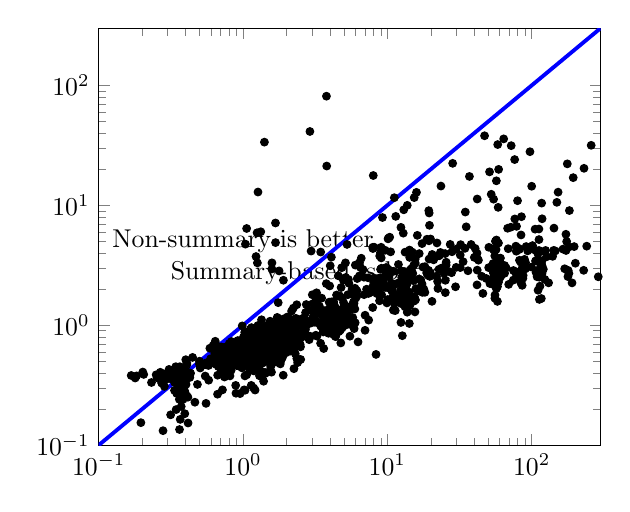
\begin{tikzpicture}[scale=0.93]
    \begin{axis}[%
    xmode=log,
    ymode=log,
    xmin=0.1,
    xmax=300,
    ymin=0.1,
    ymax=300,
    scatter/classes={%
        a={mark=o,draw=black}}]
    \draw (1, 5) node {Non-summary is better};
    \draw (3, -2) node {Summary-based is better};
    \addplot[mark=none, line width=1.5pt,blue] coordinates {(0.01,0.01) (300,300)};    
    \addplot[mark size=1.5pt,scatter,only marks,%
        scatter src=explicit symbolic]%
    table {
    x y 
    1546 12917 690 1846 Intersect:  142 s1 - s2: 548 s2 - s1: 1704
    20078.244707347447
    6018.453788592101
    35683.66937570942 335584.2864018161
    22025 22025
    0.953 0.269
    0.889 0.315
    2.252 0.434
    14.194 1.034
    360.0 1.765
    0.196 0.154
    2.508 0.518
    3.445 0.707
    1.375 0.407
    7.914 1.405
    2.359 0.527
    360.0 5.685
    360.0 2.442
    1.574 0.406
    4.756 0.712
    360.0 360.0
    360.0 2.581
    8.345 0.571
    1.899 0.383
    360.0 4.538
    1.388 0.341
    15.153 2.353
    360.0 360.0
    360.0 1.995
    1.579 0.487
    1.327 0.378
    360.0 5.523
    0.666 0.266
    12.695 0.818
    360.0 360.0
    10.996 1.337
    2.871 0.758
    13.725 1.284
    0.373 0.21
    55.654 1.787
    0.279 0.132
    0.367 0.164
    360.0 7.182
    0.344 0.198
    1.161 0.421
    1.653 0.516
    360.0 7.75
    11.035 2.817
    116.57 1.67
    2.109 0.607
    0.363 0.135
    360.0 1.733
    1.812 0.476
    1.14 0.315
    4.017 3.132
    1.257 3.31
    0.416 0.153
    1.422 0.395
    58.04 2.363
    360.0 360.0
    360.0 1.435
    360.0 9.468
    3.828 1.018
    360.0 1.489
    1.756 0.937
    360.0 360.0
    1.161 0.567
    1.153 0.653
    1.505 0.869
    360.0 6.346
    2.001 0.656
    360.0 4.322
    360.0 360.0
    360.0 2.71
    5.123 3.312
    39.151 360.0
    360.0 360.0
    360.0 7.118
    258.129 31.65
    77.53 2.724
    2.16 1.007
    1.302 0.423
    360.0 10.361
    0.303 0.38
    1.33 0.917
    7.008 1.212
    360.0 360.0
    1.036 0.699
    0.384 0.241
    2.549 1.13
    1.705 0.84
    1.355 0.864
    3.455 0.982
    360.0 10.454
    1.393 0.966
    41.784 3.993
    1.122 0.927
    1.041 0.864
    1.432 0.867
    360.0 3.782
    360.0 3.539
    1.273 0.705
    90.611 3.333
    360.0 4.503
    8.787 2.474
    56.444 360.0
    360.0 5.055
    360.0 360.0
    0.367 0.277
    360.0 4.268
    96.329 360.0
    360.0 5.113
    8.484 2.229
    360.0 4.997
    360.0 3.817
    8.968 2.925
    0.865 0.651
    0.273 0.331
    4.577 1.114
    113.311 2.684
    360.0 360.0
    360.0 360.0
    360.0 360.0
    360.0 4.437
    360.0 360.0
    4.826 3.018
    360.0 3.374
    2.253 0.64
    4.373 0.803
    1.19 0.563
    360.0 11.284
    0.344 0.338
    1.325 0.647
    1.207 0.779
    360.0 360.0
    164.686 4.312
    360.0 360.0
    78.161 4.142
    360.0 4.815
    360.0 6.051
    360.0 0.867
    1.068 0.616
    360.0 6.798
    1.027 0.873
    8.854 1.781
    93.723 4.169
    4.445 1.787
    55.48 2.71
    360.0 7.833
    0.816 0.552
    360.0 5.819
    1.053 0.516
    17.625 3.054
    360.0 6.24
    1.456 0.826
    1.604 0.717
    1.423 0.69
    1.49 0.989
    0.887 0.601
    3.026 1.142
    1.169 0.504
    360.0 18.403
    1.296 0.605
    1.904 2.372
    360.0 5.035
    11.428 8.085
    1.343 0.48
    10.107 5.253
    3.505 0.993
    12.955 2.325
    360.0 3.786
    1.796 0.77
    80.95 4.39
    1.581 0.583
    360.0 4.378
    360.0 7.022
    0.96 0.657
    52.402 12.362
    1.216 0.515
    360.0 7.834
    1.267 0.643
    0.375 0.34
    3.013 1.333
    360.0 26.286
    60.744 2.914
    360.0 360.0
    360.0 20.56
    1.624 0.535
    360.0 5.371
    360.0 5.144
    1.255 0.699
    360.0 4.072
    360.0 3.485
    4.261 1.209
    360.0 285.136
    0.902 0.565
    38.4 360.0
    1.528 0.757
    360.0 5.719
    360.0 5.214
    4.238 1.574
    1.341 0.942
    360.0 5.237
    1.283 0.853
    1.384 0.823
    360.0 9.529
    360.0 26.372
    0.396 0.256
    1.72 0.85
    360.0 2.845
    360.0 2.897
    0.314 0.371
    360.0 360.0
    56.067 2.593
    0.667 0.383
    1.086 0.701
    360.0 216.736
    360.0 5.0
    1.325 0.731
    360.0 7.757
    1.742 0.999
    22.397 2.024
    4.416 1.119
    1.254 0.836
    360.0 3.453
    360.0 4.698
    0.505 0.44
    360.0 7.596
    2.25 0.951
    6.496 3.043
    1.504 0.789
    12.945 2.73
    1.953 1.102
    1.377 0.595
    360.0 360.0
    42.74 3.487
    0.909 0.514
    360.0 360.0
    337.575 5.153
    1.594 0.819
    360.0 2.0
    13.261 4.068
    1.435 0.974
    1.952 0.926
    1.026 0.607
    360.0 4.322
    360.0 2.475
    6.162 1.765
    360.0 4.021
    0.971 0.628
    360.0 3.665
    9.708 2.635
    5.755 1.159
    3.961 0.891
    360.0 15.285
    8.91 2.245
    0.997 0.652
    360.0 33.038
    360.0 3.882
    62.019 2.646
    9.247 7.912
    1.818 0.875
    0.989 0.671
    1.387 0.513
    1.516 0.749
    190.256 2.255
    7.174 1.997
    360.0 26.986
    360.0 5.374
    360.0 48.606
    0.317 0.357
    1.363 0.882
    360.0 4.268
    360.0 39.609
    360.0 4.641
    0.717 0.403
    360.0 3.661
    0.38 0.311
    360.0 4.664
    360.0 4.696
    360.0 1.043
    360.0 5.005
    360.0 3.579
    360.0 360.0
    1.954 0.642
    360.0 3.631
    9.669 2.067
    58.123 32.114
    84.074 2.261
    360.0 5.827
    360.0 2.107
    360.0 3.776
    360.0 0.644
    0.885 0.47
    360.0 2.812
    0.363 0.37
    360.0 5.751
    1.749 0.919
    360.0 4.528
    1.599 0.812
    360.0 8.085
    360.0 4.032
    360.0 4.982
    4.866 1.679
    1.505 0.535
    0.816 0.559
    360.0 5.303
    360.0 4.676
    360.0 3.431
    360.0 360.0
    360.0 3.304
    55.447 2.564
    50.332 3.021
    360.0 360.0
    60.777 2.93
    360.0 360.0
    0.884 0.664
    0.408 0.484
    1.212 0.667
    360.0 360.0
    360.0 3.96
    360.0 0.385
    2.243 0.709
    360.0 4.973
    360.0 4.681
    1.962 0.814
    360.0 15.63
    3.911 0.972
    1.189 0.565
    3.679 1.279
    0.87 0.519
    4.093 3.696
    360.0 9.406
    0.637 0.489
    1.251 5.902
    360.0 10.424
    0.323 0.362
    2.025 0.823
    0.366 0.311
    360.0 3.829
    0.607 0.485
    360.0 6.862
    3.656 1.322
    1.017 0.289
    1.176 0.634
    360.0 4.474
    360.0 4.31
    4.472 1.346
    360.0 5.084
    4.414 0.942
    0.911 0.622
    360.0 4.268
    13.712 1.608
    1.431 0.898
    360.0 360.0
    360.0 3.366
    2.327 1.141
    360.0 5.607
    360.0 3.99
    2.17 1.312
    1.297 0.886
    360.0 360.0
    0.843 0.594
    360.0 16.416
    1.015 0.727
    360.0 3.806
    7.421 1.103
    57.568 2.375
    360.0 6.395
    16.564 2.431
    360.0 360.0
    360.0 5.528
    360.0 5.877
    1.35 0.622
    105.356 360.0
    1.766 0.899
    360.0 360.0
    5.501 0.81
    360.0 14.836
    0.831 0.596
    113.289 4.081
    360.0 4.404
    360.0 360.0
    5.412 2.238
    1.262 0.491
    2.443 0.853
    20.913 3.51
    1.601 0.853
    5.997 3.173
    360.0 5.127
    3.984 2.126
    360.0 2.687
    360.0 360.0
    360.0 18.001
    16.304 1.943
    2.209 0.984
    360.0 4.159
    360.0 21.356
    360.0 8.021
    1.546 0.808
    360.0 3.964
    4.628 0.986
    13.304 2.205
    0.67 0.582
    360.0 15.743
    14.094 1.63
    181.004 2.708
    1.216 0.596
    360.0 4.374
    0.377 0.328
    360.0 4.327
    1.164 0.628
    2.03 1.172
    1.272 0.743
    2.138 1.017
    360.0 4.365
    1.424 0.725
    360.0 282.959
    2.447 1.045
    360.0 3.741
    14.062 1.769
    360.0 8.506
    1.467 0.808
    360.0 360.0
    8.036 2.263
    360.0 360.0
    3.537 0.985
    360.0 360.0
    1.977 0.734
    0.909 0.61
    41.783 2.17
    360.0 29.116
    82.032 4.283
    116.284 2.983
    55.948 2.391
    4.194 1.143
    360.0 22.811
    12.973 1.553
    360.0 4.316
    360.0 3.139
    360.0 360.0
    360.0 4.457
    13.546 1.807
    360.0 360.0
    1.413 0.931
    360.0 5.547
    59.624 2.618
    54.437 2.757
    1.298 0.628
    56.348 360.0
    360.0 2.454
    1.758 1.045
    1.792 0.826
    360.0 3.29
    1.671 0.826
    0.372 0.357
    15.741 2.02
    2.485 0.999
    0.644 0.5
    0.987 0.987
    1.009 360.0
    360.0 360.0
    0.707 0.659
    4.773 1.177
    360.0 9.882
    0.386 0.416
    4.087 1.056
    18.77 2.749
    360.0 3.822
    360.0 4.028
    360.0 4.557
    360.0 3.116
    3.037 1.51
    360.0 4.91
    1.608 0.966
    13.734 1.71
    360.0 0.687
    2.223 1.003
    58.364 2.775
    360.0 10.421
    2.186 1.045
    5.237 1.25
    360.0 3.627
    360.0 4.8
    4.043 1.31
    360.0 5.278
    5.101 1.072
    1.792 0.565
    12.664 1.853
    1.841 0.596
    1.663 0.673
    360.0 13.325
    51.34 2.226
    2.14 0.864
    2.152 1.118
    1.263 0.748
    51.027 19.01
    24.624 2.722
    1.45 0.898
    4.203 1.436
    4.973 1.543
    1.872 0.983
    360.0 3.815
    360.0 360.0
    1.642 0.752
    1.36 0.85
    360.0 4.034
    360.0 4.729
    0.558 0.487
    21.757 360.0
    55.76 2.528
    1.857 0.739
    4.173 1.294
    360.0 3.776
    360.0 5.229
    56.946 2.424
    1.535 0.797
    58.548 9.614
    0.948 0.603
    12.812 1.851
    55.89 3.294
    14.859 4.072
    15.658 1.626
    57.218 3.221
    252.473 360.0
    360.0 2.993
    0.781 0.641
    360.0 0.796
    2.828 1.334
    360.0 2.597
    12.496 360.0
    0.657 0.491
    360.0 4.356
    5.516 1.018
    15.17 1.719
    360.0 0.585
    360.0 5.114
    360.0 360.0
    55.996 2.587
    2.013 0.887
    360.0 2.522
    360.0 4.719
    4.182 0.955
    360.0 3.554
    360.0 3.38
    115.698 2.979
    360.0 360.0
    0.369 0.273
    5.953 1.367
    1.651 0.821
    58.827 4.846
    1.539 1.08
    360.0 3.595
    28.016 4.098
    3.613 1.096
    19.464 360.0
    360.0 317.244
    360.0 11.402
    57.678 2.558
    0.896 0.592
    1.24 0.71
    0.357 0.348
    7.39 1.841
    56.153 2.9
    360.0 4.042
    360.0 3.69
    360.0 360.0
    1.643 0.823
    3.635 1.238
    1.677 0.946
    17.024 2.387
    360.0 360.0
    1.801 0.938
    360.0 3.54
    9.121 1.794
    117.756 2.685
    3.888 1.31
    1.446 0.802
    360.0 4.517
    1.519 0.772
    58.561 2.804
    360.0 8.219
    1.368 0.824
    360.0 5.434
    1.039 4.746
    1.334 0.786
    4.248 0.832
    360.0 2.373
    3.809 1.268
    360.0 5.359
    1.084 0.701
    360.0 360.0
    0.904 0.578
    104.63 4.248
    360.0 0.836
    84.62 2.832
    360.0 6.847
    360.0 344.458
    1.842 0.876
    112.471 2.771
    360.0 7.611
    360.0 4.324
    360.0 2.739
    360.0 4.594
    360.0 4.307
    360.0 7.596
    360.0 4.373
    57.49 2.69
    66.526 3.006
    2.486 360.0
    360.0 12.166
    27.855 2.741
    29.963 3.038
    1.225 0.847
    0.72 0.289
    1.213 0.615
    57.043 2.044
    7.986 17.722
    1.184 0.681
    16.127 5.616
    1.267 0.994
    360.0 5.105
    116.598 3.244
    1.479 0.701
    1.51 0.588
    0.985 0.666
    56.677 360.0
    360.0 7.662
    54.438 11.25
    99.542 3.056
    0.939 0.646
    360.0 3.919
    45.026 2.56
    1.12 0.832
    360.0 0.498
    1.469 0.756
    1.132 0.681
    63.93 35.807
    1.379 360.0
    360.0 5.394
    80.094 2.661
    360.0 360.0
    360.0 3.69
    2.256 0.932
    360.0 360.0
    312.267 1.699
    2.126 0.989
    0.363 0.35
    360.0 3.035
    3.661 1.26
    360.0 3.435
    360.0 44.532
    1.602 0.615
    0.793 0.658
    360.0 9.334
    1.679 4.887
    360.0 4.837
    360.0 29.095
    360.0 3.214
    14.238 4.235
    360.0 2.514
    1.916 0.833
    58.285 360.0
    109.741 2.869
    0.374 0.372
    1.233 0.782
    2.533 0.794
    2.185 0.954
    7.627 1.878
    19.458 3.562
    1.287 0.839
    6.591 3.621
    1.759 0.976
    4.124 1.262
    229.053 2.87
    360.0 4.534
    0.347 0.27
    1.423 0.608
    360.0 360.0
    1.795 0.782
    360.0 15.059
    360.0 360.0
    360.0 230.606
    0.66 0.65
    2.09 0.911
    360.0 4.408
    360.0 12.505
    360.0 4.178
    1.069 0.666
    360.0 3.633
    0.643 0.601
    0.577 0.462
    1.806 0.959
    0.916 0.477
    2.301 0.579
    54.388 4.343
    360.0 5.429
    345.885 35.349
    53.889 3.161
    13.242 1.425
    360.0 4.011
    87.181 2.601
    2.248 0.714
    360.0 6.015
    1.216 0.631
    360.0 4.473
    360.0 3.211
    360.0 4.251
    1.628 0.686
    360.0 4.513
    360.0 5.446
    360.0 5.142
    360.0 4.052
    6.15 1.943
    360.0 4.473
    18.197 1.882
    57.764 2.856
    360.0 45.581
    2.415 1.039
    1.341 0.885
    1.879 0.542
    1.385 0.849
    360.0 7.019
    360.0 4.087
    60.713 3.628
    172.906 4.2
    1.114 0.676
    85.802 2.986
    1.185 0.508
    8.461 1.835
    4.489 1.059
    12.222 1.613
    4.137 1.047
    360.0 17.869
    1.185 0.815
    360.0 12.682
    360.0 6.79
    1.098 0.585
    13.767 1.745
    360.0 1.824
    1.035 0.723
    85.873 2.151
    1.433 0.567
    2.918 0.809
    1.004 0.478
    360.0 360.0
    0.334 0.386
    58.972 19.937
    360.0 2.573
    0.916 0.645
    0.977 0.607
    4.048 1.403
    0.367 0.374
    1.142 0.725
    1.421 0.774
    57.119 2.765
    11.93 3.213
    360.0 13.513
    360.0 4.29
    360.0 13.329
    0.202 0.407
    61.327 2.797
    360.0 5.084
    240.43 4.563
    1.081 0.549
    110.941 2.814
    0.925 0.57
    1.472 0.726
    0.613 0.507
    64.882 2.713
    360.0 93.163
    14.709 2.734
    60.406 2.886
    1.227 0.596
    2.271 0.967
    360.0 360.0
    360.0 5.66
    1.522 0.856
    2.729 1.082
    360.0 360.0
    1.237 0.727
    360.0 3.651
    1.207 0.847
    360.0 4.398
    360.0 5.768
    25.122 3.958
    360.0 3.083
    360.0 12.042
    12.571 2.501
    58.549 2.627
    360.0 3.664
    360.0 360.0
    1.079 0.686
    360.0 54.901
    15.256 1.587
    1.413 0.751
    360.0 4.802
    360.0 360.0
    360.0 4.637
    360.0 2.611
    1.539 0.733
    2.041 0.996
    1.407 0.492
    13.014 2.805
    360.0 4.061
    360.0 5.312
    193.856 17.012
    0.29 0.381
    0.351 0.345
    360.0 4.323
    1.533 0.926
    360.0 3.502
    0.183 0.378
    0.275 0.397
    1.213 0.679
    5.493 1.34
    2.674 0.841
    1.49 0.792
    360.0 2.625
    59.254 2.925
    3.641 1.254
    360.0 14.272
    360.0 4.341
    1.679 0.992
    4.31 1.445
    2.5 0.66
    1.357 0.788
    23.787 3.002
    360.0 360.0
    360.0 360.0
    2.354 0.676
    1.059 0.682
    2.107 0.875
    58.92 2.652
    360.0 23.427
    1.4 0.837
    3.503 1.683
    360.0 4.444
    2.224 0.988
    360.0 3.827
    0.997 0.673
    360.0 13.549
    360.0 4.105
    360.0 43.814
    360.0 3.973
    360.0 2.464
    0.374 0.32
    7.165 360.0
    360.0 360.0
    360.0 11.636
    360.0 4.03
    13.616 1.492
    360.0 360.0
    360.0 360.0
    2.068 1.051
    58.444 2.842
    0.949 0.592
    360.0 4.791
    360.0 360.0
    0.831 0.53
    2.712 0.957
    360.0 3.474
    1.989 0.793
    1.952 0.934
    1.452 0.985
    360.0 360.0
    1.196 0.474
    360.0 360.0
    54.616 2.701
    1.991 1.109
    360.0 360.0
    1.03 0.378
    1.155 0.762
    4.41 1.225
    86.896 2.463
    10.127 2.924
    0.831 0.731
    5.982 1.049
    14.963 360.0
    360.0 4.122
    0.298 0.357
    124.756 4.204
    13.487 1.584
    56.943 5.138
    2.359 0.808
    3.778 1.163
    16.784 2.045
    0.428 0.367
    0.984 0.441
    360.0 5.181
    1.007 0.684
    1.232 0.665
    360.0 360.0
    360.0 3.191
    1.716 0.806
    360.0 360.0
    3.847 1.12
    360.0 6.795
    360.0 5.728
    360.0 360.0
    360.0 5.678
    360.0 360.0
    360.0 5.778
    0.972 0.596
    360.0 13.001
    360.0 4.521
    0.383 0.372
    1.81 0.794
    360.0 5.197
    360.0 66.977
    54.136 2.912
    360.0 360.0
    0.919 0.745
    360.0 360.0
    1.386 0.807
    1.57 0.828
    58.067 3.22
    360.0 360.0
    0.403 0.321
    360.0 7.568
    29.927 4.308
    360.0 3.75
    1.354 0.773
    0.893 0.271
    1.482 0.701
    360.0 13.219
    360.0 360.0
    58.508 3.225
    360.0 3.578
    78.519 6.678
    0.386 0.362
    360.0 4.624
    2.047 0.971
    360.0 2.634
    360.0 360.0
    1.764 0.904
    141.935 4.208
    360.0 3.959
    360.0 3.827
    1.455 0.65
    1.584 0.728
    360.0 2.917
    5.882 0.937
    9.064 3.644
    1.526 0.654
    3.39 1.052
    15.363 1.731
    1.618 0.798
    360.0 3.196
    0.942 0.73
    0.232 0.333
    1.057 0.726
    360.0 3.557
    360.0 4.789
    360.0 6.74
    360.0 6.343
    9.926 1.535
    53.926 3.265
    360.0 360.0
    360.0 4.651
    10.53 4.091
    1.423 0.903
    360.0 2.942
    97.244 27.991
    11.795 2.243
    360.0 4.071
    3.754 1.0
    4.274 1.206
    0.362 0.241
    1.703 1.011
    1.513 0.785
    1.224 0.688
    360.0 4.06
    3.582 0.923
    360.0 5.858
    360.0 6.65
    1.617 0.704
    360.0 360.0
    14.993 2.708
    360.0 4.87
    1.798 0.734
    10.25 2.529
    0.98 0.653
    1.812 0.867
    360.0 4.939
    56.116 2.411
    5.151 1.004
    1.349 0.65
    360.0 47.85
    56.894 2.021
    360.0 6.133
    360.0 2.113
    1.21 0.702
    1.209 0.56
    15.588 3.566
    360.0 17.005
    2.487 0.691
    360.0 18.366
    360.0 4.787
    1.204 0.628
    360.0 360.0
    1.271 0.852
    1.723 1.001
    0.7 0.584
    360.0 4.311
    360.0 4.116
    1.679 0.816
    0.545 0.469
    3.783 81.256
    360.0 360.0
    360.0 4.042
    34.671 8.789
    0.939 0.573
    360.0 360.0
    360.0 4.177
    2.086 0.82
    1.521 0.734
    360.0 3.644
    154.748 360.0
    5.825 1.783
    0.832 0.503
    0.85 360.0
    55.363 2.597
    360.0 0.641
    1.245 0.506
    42.14 3.586
    1.801 0.686
    360.0 217.574
    4.021 1.254
    1.658 0.701
    57.68 2.825
    5.014 1.123
    360.0 15.713
    360.0 360.0
    54.702 2.859
    360.0 5.253
    1.098 0.544
    0.354 0.342
    3.719 1.279
    360.0 360.0
    1.102 0.648
    1.53 0.781
    360.0 7.563
    9.654 4.217
    1.027 0.729
    360.0 5.426
    2.501 1.045
    3.172 360.0
    1.269 12.904
    1.12 0.527
    1.794 0.667
    1.796 0.803
    60.602 2.521
    40.557 4.373
    1.333 0.508
    3.6 0.927
    0.336 0.333
    360.0 39.551
    360.0 360.0
    0.375 0.406
    360.0 3.214
    360.0 13.207
    360.0 3.695
    80.091 2.765
    360.0 5.374
    360.0 3.74
    360.0 5.188
    360.0 8.664
    3.695 1.168
    1.185 0.488
    360.0 360.0
    360.0 5.22
    2.339 1.01
    360.0 360.0
    15.61 3.299
    1.197 0.681
    360.0 50.698
    5.812 1.553
    360.0 12.558
    360.0 2.881
    360.0 4.234
    360.0 3.826
    0.876 0.49
    360.0 3.946
    360.0 2.834
    360.0 21.744
    58.992 2.75
    1.03 0.573
    1.398 0.76
    0.433 0.398
    360.0 37.672
    4.693 1.735
    4.276 1.002
    0.804 0.653
    360.0 360.0
    360.0 24.039
    13.109 2.084
    360.0 5.917
    2.126 0.919
    360.0 3.374
    0.408 0.469
    17.865 2.005
    57.296 2.86
    1.245 0.655
    19.48 8.627
    360.0 5.409
    360.0 7.113
    0.927 0.541
    0.387 0.35
    1.697 0.493
    360.0 4.98
    1.901 0.684
    360.0 24.222
    4.009 1.012
    58.623 3.574
    54.063 2.413
    2.022 0.888
    360.0 102.988
    360.0 3.905
    1.646 0.672
    4.243 1.302
    4.104 1.076
    360.0 360.0
    1.894 1.074
    12.41 6.548
    10.816 2.806
    360.0 1.031
    1.266 0.593
    19.409 5.057
    360.0 360.0
    12.611 2.202
    10.271 2.035
    1.582 0.911
    12.46 1.557
    1.316 0.76
    3.949 1.558
    1.567 0.878
    360.0 19.271
    0.872 0.663
    360.0 4.933
    41.906 11.289
    360.0 4.245
    360.0 360.0
    1.654 0.903
    360.0 4.268
    1.721 0.657
    1.588 0.728
    360.0 360.0
    360.0 360.0
    1.595 1.013
    360.0 28.912
    360.0 4.585
    0.343 0.342
    1.998 0.973
    0.906 0.496
    0.984 0.624
    1.775 0.774
    360.0 6.333
    360.0 3.299
    360.0 5.063
    5.369 2.409
    5.321 1.797
    360.0 6.729
    1.181 0.572
    4.721 0.91
    0.554 0.223
    360.0 3.391
    152.334 12.875
    360.0 360.0
    360.0 2.853
    1.718 0.975
    360.0 6.31
    1.938 0.942
    360.0 2.192
    1.577 0.877
    360.0 3.642
    360.0 3.279
    360.0 360.0
    0.928 0.619
    0.408 0.258
    55.456 2.474
    2.712 1.275
    360.0 2.044
    360.0 3.54
    360.0 3.707
    0.39 0.341
    360.0 3.569
    0.812 0.378
    360.0 15.95
    3.547 1.019
    1.989 0.733
    1.807 0.96
    58.357 3.216
    1.222 0.815
    360.0 6.672
    0.307 0.428
    0.972 0.619
    0.301 0.374
    22.282 2.319
    1.865 0.979
    360.0 1.356
    360.0 4.131
    3.397 1.359
    360.0 11.636
    1.61 0.647
    4.654 1.296
    1.469 0.565
    360.0 4.543
    3.052 1.073
    112.789 3.459
    1.157 0.686
    15.277 1.694
    0.371 0.352
    1.108 0.874
    3.303 1.25
    0.316 0.409
    1.719 0.704
    360.0 2.609
    0.784 0.486
    15.524 1.291
    114.025 3.301
    1.357 0.621
    4.19 1.073
    360.0 3.181
    116.639 3.097
    1.777 0.797
    360.0 360.0
    360.0 2.92
    1.381 0.667
    0.387 0.365
    1.971 0.587
    117.974 7.723
    330.388 360.0
    1.475 0.904
    360.0 360.0
    3.773 1.212
    2.906 41.276
    1.168 0.852
    1.006 0.796
    1.76 0.647
    3.773 1.117
    1.516 0.614
    2.66 1.155
    0.781 0.41
    3.932 1.134
    0.874 0.616
    31.98 3.85
    360.0 31.193
    1.009 0.559
    10.181 5.325
    360.0 360.0
    1.294 0.43
    360.0 7.546
    117.74 3.147
    0.975 0.563
    9.36 2.232
    1.912 1.13
    3.905 1.351
    1.742 0.94
    3.907 0.857
    1.236 0.533
    360.0 360.0
    360.0 4.035
    1.752 1.543
    1.824 0.575
    360.0 4.798
    1.817 0.811
    2.348 0.771
    1.023 0.67
    10.878 2.082
    1.787 1.082
    4.691 1.063
    360.0 5.306
    12.499 2.237
    360.0 247.137
    5.232 360.0
    1.45 0.705
    2.383 0.76
    338.716 6.194
    0.38 0.38
    178.78 2.866
    1.818 0.802
    1.592 0.489
    1.535 0.677
    182.4 9.042
    2.353 0.865
    2.057 0.797
    360.0 5.393
    57.601 2.657
    1.083 0.617
    0.738 0.476
    7.872 2.062
    3.725 0.984
    3.272 1.601
    360.0 5.677
    1.005 0.652
    360.0 7.136
    130.889 2.257
    360.0 3.283
    360.0 2.35
    1.493 0.796
    2.487 0.814
    360.0 360.0
    5.878 1.521
    13.73 9.994
    1.418 0.777
    10.373 5.422
    360.0 4.079
    360.0 6.169
    2.209 0.957
    360.0 12.095
    1.844 0.957
    2.229 1.388
    360.0 7.811
    1.743 0.557
    360.0 4.592
    1.15 0.446
    1.661 0.911
    360.0 360.0
    1.265 0.587
    360.0 7.996
    360.0 1.042
    0.827 0.421
    21.605 360.0
    360.0 360.0
    4.099 1.565
    360.0 4.134
    360.0 14.636
    54.311 4.275
    85.277 360.0
    3.379 1.443
    4.611 0.884
    1.243 0.531
    1.051 0.603
    360.0 360.0
    4.95 1.193
    0.346 0.377
    0.9 0.603
    72.077 31.44
    360.0 4.647
    1.218 0.62
    0.393 0.357
    1.322 0.848
    360.0 6.972
    1.767 0.89
    1.245 0.555
    360.0 2.627
    360.0 2.883
    360.0 271.167
    0.743 0.654
    360.0 6.969
    360.0 360.0
    4.68 0.929
    1.359 0.539
    13.255 2.162
    360.0 4.005
    360.0 4.839
    0.783 0.545
    360.0 3.819
    0.322 0.394
    77.673 4.563
    6.899 1.799
    13.84 1.411
    360.0 8.233
    48.401 2.455
    10.715 1.939
    1.071 0.675
    360.0 2.595
    56.895 16.006
    1.289 0.808
    89.177 3.541
    6.4 3.324
    0.807 0.551
    360.0 8.103
    1.967 0.8
    59.228 2.763
    360.0 5.948
    0.38 0.395
    4.504 1.318
    0.499 0.501
    1.875 1.04
    1.737 0.843
    360.0 255.844
    0.338 0.406
    360.0 4.183
    1.129 0.6
    1.951 1.039
    360.0 4.518
    0.798 0.673
    0.402 0.365
    360.0 360.0
    360.0 14.555
    1.384 0.759
    0.769 0.573
    360.0 9.13
    360.0 4.912
    11.265 1.744
    350.53 6.532
    0.362 0.384
    0.905 0.461
    360.0 3.222
    0.413 0.407
    360.0 4.381
    0.707 0.44
    360.0 6.974
    360.0 4.08
    1.283 0.605
    56.872 2.621
    0.352 0.372
    1.218 0.743
    1.664 0.691
    360.0 360.0
    0.267 0.405
    360.0 2.412
    0.884 0.582
    1.958 0.625
    1.195 0.731
    8.693 1.985
    0.828 0.482
    360.0 360.0
    360.0 1.878
    12.518 1.511
    1.401 0.678
    360.0 0.686
    114.71 2.847
    1.377 0.708
    360.0 9.891
    360.0 174.097
    2.389 0.488
    360.0 21.218
    82.244 2.498
    360.0 3.751
    360.0 360.0
    10.684 2.247
    360.0 1.224
    1.777 2.838
    360.0 2.754
    0.578 0.348
    1.275 0.678
    1.186 0.299
    2.253 0.742
    0.701 0.486
    360.0 4.557
    360.0 4.209
    1.544 360.0
    1.849 0.711
    1.54 0.947
    360.0 3.894
    0.377 0.269
    360.0 10.877
    360.0 7.468
    360.0 6.957
    360.0 71.783
    2.141 1.049
    360.0 4.73
    360.0 33.351
    360.0 4.943
    360.0 2.247
    1.438 0.631
    360.0 8.46
    0.369 0.411
    360.0 3.585
    2.01 0.797
    1.303 0.726
    360.0 4.307
    360.0 3.947
    1.346 0.887
    149.354 10.588
    0.363 0.36
    32.007 3.025
    0.272 0.37
    360.0 4.008
    1.723 1.038
    1.059 0.386
    360.0 360.0
    1.724 1.162
    360.0 4.126
    360.0 360.0
    33.467 3.387
    360.0 6.504
    74.713 2.86
    360.0 3.878
    1.117 0.581
    1.535 0.949
    360.0 360.0
    57.298 3.117
    360.0 77.015
    14.598 1.677
    0.596 0.485
    360.0 2.215
    102.005 360.0
    2.173 0.963
    1.656 0.682
    12.988 9.175
    4.159 1.175
    116.712 360.0
    60.436 2.76
    0.596 0.525
    1.145 0.955
    169.218 2.957
    360.0 9.426
    360.0 0.559
    360.0 360.0
    3.73 1.282
    360.0 4.727
    360.0 360.0
    1.509 1.019
    2.082 1.097
    360.0 360.0
    360.0 360.0
    360.0 3.762
    360.0 85.744
    360.0 3.123
    360.0 2.54
    360.0 5.863
    360.0 5.543
    1.52 0.698
    79.762 10.926
    0.383 0.304
    5.961 2.034
    0.805 0.484
    2.19 0.929
    1.587 0.781
    6.051 1.686
    0.168 0.381
    1.286 0.657
    360.0 2.816
    1.089 0.733
    4.135 1.518
    110.254 3.955
    360.0 2.882
    360.0 3.964
    1.225 0.815
    1.381 0.748
    360.0 28.526
    7.359 2.485
    0.365 0.451
    1.369 0.904
    1.183 0.531
    1.207 0.604
    55.96 2.743
    360.0 4.932
    360.0 4.083
    1.369 0.637
    3.25 0.811
    360.0 360.0
    0.378 0.33
    360.0 14.162
    0.964 0.612
    360.0 3.279
    8.317 2.447
    360.0 6.694
    68.724 4.347
    56.8 360.0
    0.987 0.509
    360.0 29.83
    360.0 3.633
    360.0 3.138
    1.71 1.022
    99.927 14.42
    1.161 0.88
    360.0 360.0
    56.63 4.276
    74.512 2.378
    1.844 0.822
    360.0 360.0
    0.337 0.357
    1.968 0.886
    54.706 2.72
    1.863 0.611
    8.1 4.473
    14.566 2.947
    360.0 5.105
    360.0 3.389
    360.0 63.455
    360.0 4.772
    1.287 0.506
    1.681 0.799
    360.0 2.982
    360.0 7.189
    1.33 0.954
    360.0 4.398
    54.47 2.178
    0.763 0.462
    360.0 22.776
    0.391 0.363
    1.622 0.607
    6.264 0.726
    360.0 6.633
    360.0 4.749
    0.805 0.591
    0.254 0.364
    360.0 4.711
    61.426 2.987
    28.329 22.39
    311.163 360.0
    29.657 2.092
    360.0 3.47
    360.0 5.066
    4.21 1.065
    360.0 4.603
    360.0 2.767
    0.933 0.579
    1.576 0.699
    56.111 2.571
    58.781 2.526
    12.882 5.859
    1.457 0.685
    41.926 2.882
    114.106 2.117
    35.155 6.616
    50.472 4.463
    85.412 3.387
    1.238 0.634
    360.0 14.32
    360.0 360.0
    1.955 0.741
    3.127 1.099
    1.104 0.561
    0.967 0.638
    0.949 0.491
    360.0 360.0
    1.222 0.532
    2.552 0.798
    360.0 110.748
    13.203 2.562
    5.694 1.998
    110.635 1.958
    3.799 21.257
    360.0 4.77
    55.836 2.743
    11.166 1.515
    0.394 0.381
    360.0 3.562
    360.0 13.784
    4.149 1.288
    360.0 1.278
    360.0 8.368
    37.02 17.411
    0.962 0.73
    1.168 0.645
    8.845 3.781
    360.0 360.0
    0.639 0.509
    360.0 4.631
    360.0 360.0
    8.55 2.384
    360.0 3.842
    0.649 0.608
    360.0 17.421
    13.34 1.987
    14.43 3.969
    55.24 2.683
    1.496 0.692
    9.048 4.469
    4.215 1.005
    1.952 0.997
    360.0 10.481
    360.0 3.558
    1.917 0.758
    1.144 0.634
    360.0 43.905
    360.0 2.34
    360.0 2.182
    59.001 2.86
    117.944 2.829
    1.454 0.733
    200.624 3.29
    4.3 1.438
    360.0 12.576
    123.271 2.409
    91.499 4.53
    19.364 9.028
    360.0 3.822
    56.996 2.586
    360.0 3.211
    360.0 12.737
    360.0 10.891
    360.0 3.827
    0.447 0.539
    1.836 0.671
    12.419 1.055
    3.019 1.796
    360.0 360.0
    17.38 4.793
    360.0 360.0
    1.446 0.976
    360.0 3.31
    1.759 1.067
    360.0 360.0
    25.538 3.355
    360.0 30.959
    360.0 0.635
    360.0 360.0
    0.372 0.272
    1.103 0.771
    9.472 2.493
    174.622 4.988
    2.208 1.036
    56.819 2.969
    176.382 22.17
    1.503 0.558
    0.958 0.644
    57.043 2.77
    360.0 360.0
    360.0 2.287
    263.634 360.0
    3.765 1.036
    360.0 3.751
    360.0 4.981
    1.214 0.827
    0.523 360.0
    1.664 0.679
    13.243 2.201
    360.0 2.336
    360.0 3.205
    1.256 0.914
    1.832 0.898
    1.336 360.0
    1.557 0.682
    360.0 11.57
    360.0 2.193
    0.773 0.58
    0.803 0.653
    360.0 4.943
    360.0 360.0
    2.066 0.922
    360.0 4.382
    360.0 3.185
    5.005 1.054
    28.661 360.0
    10.831 1.701
    1.586 3.313
    360.0 6.533
    1.23 3.74
    15.155 1.664
    112.145 6.346
    0.339 0.401
    1.833 0.973
    0.629 0.523
    360.0 4.754
    360.0 360.0
    115.404 2.902
    0.375 0.36
    55.635 2.778
    4.671 1.757
    0.393 0.422
    2.02 0.783
    230.287 20.352
    360.0 1.222
    360.0 360.0
    360.0 7.652
    40.021 3.678
    360.0 2.723
    1.06 0.696
    360.0 7.05
    0.702 0.522
    1.369 0.856
    1.678 0.639
    360.0 360.0
    360.0 5.031
    1.34 0.716
    360.0 5.277
    360.0 4.324
    1.934 1.076
    360.0 32.133
    0.932 0.458
    360.0 5.333
    3.266 1.053
    360.0 13.951
    57.787 2.747
    360.0 3.709
    1.798 1.054
    0.395 0.183
    1.174 0.908
    360.0 4.483
    6.881 2.515
    0.621 0.678
    60.75 3.259
    360.0 3.201
    360.0 4.663
    360.0 360.0
    1.066 0.834
    1.585 0.966
    3.729 1.292
    1.581 0.725
    4.028 1.388
    360.0 4.402
    112.495 4.198
    12.007 1.623
    0.342 0.451
    3.774 2.222
    360.0 2.748
    360.0 4.993
    0.179 0.363
    14.919 1.643
    0.97 0.52
    3.674 0.94
    59.391 2.448
    1.048 0.464
    0.789 0.582
    13.351 2.068
    2.139 1.022
    1.601 0.93
    0.801 0.605
    360.0 4.11
    1.935 0.979
    360.0 4.469
    360.0 2.507
    1.639 0.994
    0.37 0.363
    360.0 11.499
    3.202 1.603
    3.865 0.877
    360.0 3.703
    360.0 45.106
    0.665 0.487
    5.254 4.718
    2.307 0.776
    360.0 4.216
    54.869 2.568
    1.336 0.724
    360.0 0.848
    7.981 2.462
    1.91 0.956
    0.959 0.695
    4.306 1.28
    0.731 0.496
    4.57 2.584
    59.102 2.701
    360.0 6.292
    351.388 85.278
    360.0 6.438
    360.0 17.465
    58.519 3.218
    360.0 360.0
    360.0 3.27
    360.0 2.16
    360.0 21.18
    1.311 360.0
    360.0 9.6
    57.457 3.36
    101.315 4.615
    1.8 0.895
    0.38 0.292
    1.207 0.692
    3.595 0.879
    360.0 4.387
    360.0 5.598
    0.388 0.418
    9.094 2.987
    1.619 0.978
    360.0 2.08
    360.0 4.116
    349.262 4.348
    360.0 9.4
    360.0 4.779
    360.0 8.645
    1.799 0.892
    360.0 6.025
    1.3 0.379
    1.974 0.873
    5.566 1.125
    360.0 35.715
    2.283 0.901
    1.856 0.664
    360.0 3.86
    360.0 4.152
    1.813 0.675
    360.0 5.273
    360.0 22.929
    1.968 0.674
    360.0 0.695
    360.0 3.796
    1.577 0.811
    360.0 9.248
    360.0 2.255
    1.839 0.874
    360.0 4.378
    360.0 3.598
    1.669 0.695
    1.784 0.984
    1.055 0.498
    1.131 0.721
    360.0 3.149
    0.734 0.638
    4.237 1.553
    1.103 0.44
    1.236 0.552
    59.043 2.987
    55.024 2.716
    1.173 0.706
    25.234 2.369
    360.0 18.323
    360.0 360.0
    1.405 0.829
    1.189 0.715
    1.657 0.504
    0.82 0.448
    0.759 0.616
    360.0 7.613
    1.464 0.642
    178.145 2.544
    3.452 4.076
    360.0 77.588
    360.0 360.0
    360.0 360.0
    360.0 49.203
    360.0 360.0
    56.072 3.204
    360.0 360.0
    0.972 0.67
    1.837 0.691
    360.0 2.354
    3.976 0.947
    22.835 3.794
    360.0 5.378
    112.118 2.759
    360.0 4.748
    14.124 2.372
    0.849 0.632
    0.395 0.281
    18.798 5.212
    360.0 15.309
    1.656 0.811
    1.055 0.629
    360.0 12.002
    360.0 5.592
    18.775 2.715
    8.823 1.598
    1.093 0.634
    1.087 0.538
    90.322 2.952
    112.769 2.516
    360.0 8.941
    1.808 0.935
    38.023 4.714
    110.62 2.611
    360.0 3.994
    360.0 4.854
    0.25 0.386
    360.0 24.533
    360.0 3.816
    17.482 1.88
    360.0 4.713
    360.0 360.0
    360.0 360.0
    0.891 0.643
    360.0 360.0
    17.191 2.0
    360.0 10.083
    360.0 6.42
    360.0 2.474
    360.0 5.809
    360.0 318.395
    0.264 0.374
    360.0 3.688
    0.922 0.652
    360.0 4.264
    117.151 10.431
    1.311 0.677
    360.0 33.234
    360.0 4.489
    0.547 0.377
    9.905 3.002
    360.0 0.591
    4.951 2.378
    36.176 2.846
    2.1 0.773
    105.504 6.326
    2.18 0.815
    360.0 13.463
    0.563 0.467
    1.72 0.771
    360.0 23.248
    55.386 2.955
    0.379 0.379
    3.839 1.17
    360.0 2.847
    360.0 3.968
    56.27 2.845
    360.0 2.424
    1.12 0.663
    360.0 26.988
    360.0 3.793
    34.483 4.377
    3.179 1.087
    360.0 0.522
    360.0 4.415
    360.0 4.63
    0.388 0.361
    360.0 3.638
    360.0 8.696
    360.0 10.039
    1.063 0.683
    360.0 54.474
    360.0 4.697
    360.0 5.743
    360.0 360.0
    360.0 21.799
    360.0 0.707
    117.999 2.8
    360.0 360.0
    360.0 1.137
    0.705 0.425
    57.859 1.58
    360.0 0.402
    1.549 0.597
    2.048 0.658
    360.0 7.43
    68.058 6.435
    1.218 0.658
    360.0 296.536
    116.266 2.812
    360.0 3.262
    360.0 4.505
    360.0 3.643
    107.198 2.749
    360.0 4.312
    360.0 10.992
    360.0 0.789
    3.932 1.27
    5.047 1.109
    360.0 2.718
    1.826 0.695
    360.0 5.235
    19.482 2.765
    1.328 0.634
    12.329 1.96
    0.285 0.309
    0.342 0.374
    40.263 360.0
    1.19 0.416
    23.075 3.877
    8.474 2.368
    360.0 3.075
    1.6 0.73
    360.0 360.0
    360.0 7.367
    38.883 360.0
    360.0 0.681
    4.731 1.335
    360.0 0.602
    360.0 0.589
    2.356 1.482
    23.305 4.045
    360.0 5.886
    360.0 1.931
    0.972 0.6
    360.0 40.241
    156.631 360.0
    360.0 3.114
    360.0 3.416
    360.0 37.869
    360.0 26.754
    1.406 33.643
    1.345 0.718
    360.0 0.843
    0.851 0.633
    0.373 0.249
    360.0 3.61
    360.0 2.913
    55.471 3.79
    360.0 3.911
    1.352 0.87
    1.703 0.981
    360.0 360.0
    2.159 0.994
    116.38 360.0
    360.0 12.243
    360.0 4.913
    329.878 4.25
    360.0 0.981
    1.107 0.562
    1.161 0.669
    1.309 0.683
    360.0 0.836
    58.386 3.143
    115.204 2.978
    360.0 4.049
    5.256 1.274
    1.249 0.513
    360.0 2.982
    360.0 5.939
    1.597 0.823
    4.194 1.031
    1.801 0.902
    360.0 360.0
    1.219 0.853
    1.223 0.491
    360.0 4.348
    0.814 0.431
    360.0 0.868
    2.077 0.89
    360.0 0.524
    360.0 0.705
    1.599 0.852
    360.0 0.398
    360.0 360.0
    360.0 0.609
    360.0 5.378
    360.0 0.987
    360.0 2.735
    360.0 174.376
    360.0 5.273
    360.0 5.93
    19.278 2.87
    360.0 0.864
    360.0 360.0
    0.677 0.663
    360.0 2.888
    3.193 0.825
    360.0 360.0
    360.0 4.455
    360.0 2.602
    360.0 5.072
    0.975 0.654
    7.931 4.466
    1.081 0.798
    360.0 16.598
    0.887 0.621
    360.0 2.692
    61.525 2.612
    10.028 2.655
    139.515 3.752
    3.209 1.369
    1.338 0.772
    112.273 5.177
    1.408 360.0
    0.652 0.47
    13.173 1.555
    1.722 0.744
    1.789 0.869
    1.033 0.287
    2.368 1.053
    0.573 0.479
    360.0 360.0
    1.331 0.884
    360.0 15.103
    360.0 5.618
    360.0 0.764
    57.914 2.101
    71.661 6.569
    11.336 1.788
    11.203 360.0
    4.778 2.063
    1.413 0.753
    3.622 1.103
    7.941 4.359
    360.0 12.627
    1.301 0.658
    360.0 360.0
    0.979 0.687
    360.0 360.0
    0.386 0.378
    0.35 0.296
    360.0 5.096
    360.0 2.709
    0.637 0.586
    13.211 1.614
    360.0 0.467
    1.445 0.546
    47.129 38.014
    360.0 1.901
    6.78 2.911
    3.518 1.333
    1.584 2.945
    1.554 0.45
    360.0 1.038
    360.0 360.0
    1.69 0.968
    1.346 0.869
    360.0 1.144
    11.34 1.325
    27.236 4.723
    360.0 2.826
    360.0 5.825
    126.618 3.72
    22.052 4.853
    360.0 3.805
    8.955 4.024
    360.0 4.016
    360.0 0.73
    1.698 0.581
    142.63 6.453
    4.015 1.293
    360.0 0.367
    84.884 8.038
    2.007 0.879
    3.621 0.639
    360.0 9.25
    1.976 0.969
    360.0 6.166
    1.914 0.801
    360.0 3.595
    1.603 0.803
    360.0 3.277
    55.216 2.195
    360.0 360.0
    55.557 1.679
    21.894 2.559
    360.0 0.499
    0.92 0.543
    360.0 0.715
    1.21 0.634
    1.384 0.857
    360.0 3.0
    360.0 360.0
    360.0 5.271
    360.0 1.298
    12.151 1.758
    1.761 0.658
    360.0 360.0
    1.573 0.795
    360.0 5.726
    3.73 1.003
    360.0 2.693
    1.327 6.018
    360.0 5.366
    0.759 0.542
    3.069 1.273
    10.048 1.639
    5.329 1.043
    1.734 0.646
    360.0 35.787
    4.008 1.024
    360.0 0.608
    20.421 3.893
    0.631 0.52
    1.547 0.736
    1.752 0.841
    3.766 0.969
    19.578 6.809
    5.136 2.502
    0.367 0.355
    58.897 2.292
    0.415 0.251
    54.125 360.0
    1.086 0.627
    360.0 18.37
    360.0 360.0
    360.0 92.253
    3.234 1.864
    1.883 0.883
    360.0 0.649
    120.343 2.932
    360.0 0.781
    360.0 11.034
    196.813 4.526
    1.229 0.58
    360.0 8.382
    2.225 0.746
    360.0 2.382
    360.0 3.595
    18.138 3.063
    360.0 2.779
    1.03 0.583
    57.383 2.801
    360.0 5.955
    1.275 0.649
    360.0 69.363
    26.172 2.816
    360.0 5.356
    360.0 1.082
    360.0 4.938
    360.0 0.62
    360.0 0.99
    15.906 12.826
    360.0 8.695
    360.0 6.073
    12.421 2.839
    172.579 5.734
    360.0 360.0
    55.196 2.786
    1.445 0.784
    360.0 19.642
    34.811 360.0
    53.13 2.248
    360.0 0.826
    360.0 51.112
    1.191 0.635
    360.0 6.661
    360.0 3.818
    181.241 4.496
    360.0 0.337
    1.678 7.124
    360.0 4.037
    1.47 0.659
    360.0 2.402
    3.904 1.336
    0.401 0.516
    3.665 0.992
    1.216 0.616
    360.0 2.579
    9.748 360.0
    2.004 0.97
    360.0 0.339
    360.0 4.525
    360.0 0.563
    1.482 0.908
    360.0 1.665
    4.419 0.913
    4.414 1.299
    360.0 1.537
    1.212 0.288
    360.0 2.076
    4.346 1.152
    360.0 0.905
    14.234 1.524
    360.0 360.0
    360.0 0.441
    2.196 0.734
    360.0 4.531
    360.0 0.515
    56.045 5.018
    360.0 0.763
    1.991 1.018
    360.0 1.139
    15.393 1.705
    360.0 4.664
    4.943 1.4
    360.0 1.82
    2.452 0.713
    19.662 2.554
    360.0 2.041
    2.144 0.928
    360.0 0.643
    55.859 2.378
    360.0 14.951
    0.744 0.37
    360.0 0.648
    360.0 1.927
    289.087 2.535
    360.0 1.173
    360.0 2.657
    360.0 0.341
    360.0 2.284
    360.0 2.248
    360.0 10.288
    360.0 360.0
    360.0 0.591
    360.0 360.0
    360.0 14.485
    360.0 0.538
    360.0 3.175
    360.0 0.614
    360.0 1.96
    360.0 4.756
    360.0 0.506
    360.0 4.937
    360.0 0.817
    360.0 4.234
    360.0 4.474
    360.0 4.26
    360.0 1.08
    360.0 19.922
    360.0 3.34
    14.269 3.677
    360.0 3.68
    1.528 0.818
    360.0 0.361
    360.0 1.041
    0.372 0.365
    360.0 3.161
    360.0 3.369
    1.174 0.618
    360.0 4.615
    22.771 2.927
    360.0 1.615
    360.0 0.655
    360.0 4.81
    360.0 360.0
    360.0 7.175
    360.0 0.444
    2.642 0.932
    4.86 0.95
    360.0 3.604
    360.0 3.484
    3.954 1.087
    360.0 52.247
    360.0 2.272
    360.0 3.935
    13.687 360.0
    360.0 0.635
    360.0 0.405
    2.742 1.488
    15.211 3.155
    360.0 5.719
    57.074 2.66
    360.0 1.074
    360.0 38.115
    360.0 7.407
    360.0 3.209
    360.0 1.03
    360.0 1.103
    360.0 11.341
    360.0 3.967
    360.0 1.288
    360.0 15.765
    360.0 0.339
    360.0 0.603
    360.0 6.399
    360.0 0.514
    360.0 0.785
    360.0 0.903
    360.0 0.688
    360.0 4.261
    360.0 360.0
    360.0 0.352
    360.0 43.239
    360.0 3.989
    360.0 1.005
    360.0 71.567
    360.0 0.485
    360.0 0.532
    69.245 2.191
    3.962 1.023
    360.0 7.039
    360.0 2.11
    360.0 4.477
    360.0 6.736
    0.205 0.389
    360.0 1.752
    360.0 360.0
    113.013 1.641
    360.0 10.861
    360.0 0.823
    360.0 12.829
    360.0 2.727
    360.0 0.838
    360.0 3.04
    360.0 4.049
    360.0 6.344
    76.172 24.068
    145.569 4.165
    0.387 0.428
    360.0 4.366
    0.802 0.703
    45.892 1.841
    360.0 2.785
    360.0 4.567
    360.0 3.926
    9.366 2.321
    1.272 0.623
    2.471 0.851
    5.532 1.433
    55.052 2.974
    360.0 5.657
    4.329 1.172
    0.335 0.286
    360.0 5.046
    1.842 0.516
    360.0 360.0
    1.073 0.616
    1.343 1.111
    360.0 1.21
    360.0 4.155
    6.398 2.579
    1.246 0.847
    4.383 0.825
    14.196 1.763
    1.265 0.587
    1.737 1.148
    360.0 12.908
    9.471 2.182
    360.0 0.573
    360.0 1.408
    2.681 0.846
    360.0 360.0
    360.0 0.91
    3.589 1.054
    16.618 3.958
    1.407 0.642
    0.277 0.337
    0.403 0.351
    0.284 0.382
    360.0 1.59
    0.365 0.315
    360.0 0.662
    360.0 4.393
    360.0 2.823
    8.899 2.256
    13.856 1.73
    360.0 7.291
    360.0 360.0
    0.377 0.371
    360.0 6.392
    360.0 5.494
    360.0 4.978
    1.426 0.69
    360.0 0.751
    0.385 0.365
    360.0 0.58
    360.0 6.596
    0.358 0.364
    360.0 4.799
    360.0 0.91
    360.0 0.619
    2.962 4.153
    0.483 0.321
    360.0 2.106
    360.0 7.368
    0.675 0.452
    360.0 8.582
    360.0 2.555
    6.182 2.451
    7.845 2.014
    0.795 0.588
    360.0 3.64
    360.0 3.584
    360.0 0.75
    25.529 3.178
    360.0 5.24
    56.627 2.477
    360.0 0.883
    3.143 1.059
    360.0 3.355
    360.0 5.144
    360.0 0.396
    360.0 1.387
    360.0 1.49
    360.0 0.793
    360.0 0.766
    360.0 0.471
    360.0 94.405
    360.0 6.182
    4.008 1.296
    360.0 46.864
    360.0 3.994
    0.381 0.385
    2.703 0.915
    1.74 0.883
    20.373 1.582
    0.986 0.587
    0.642 0.735
    13.126 2.592
    4.034 1.432
    1.059 6.408
    23.495 14.471
    360.0 4.56
    2.941 1.041
    0.499 0.475
    0.266 0.391
    5.82 1.467
    360.0 5.689
    360.0 360.0
    4.18 1.04
    360.0 2.26
    360.0 0.372
    0.464 0.228
    360.0 0.478
    109.031 2.534
    360.0 360.0
    360.0 0.452
    1.262 0.622
    1.408 0.568
    1.494 0.709
    2.442 0.756
    360.0 3.753
    0.903 0.682
    360.0 0.382
    1.091 0.742
    360.0 4.172
    0.644 0.552
    360.0 9.753
    360.0 5.59
    0.348 0.274
    360.0 16.066
    1.837 0.904
    0.76 0.513
    360.0 360.0
    1.369 0.637
    360.0 0.35
    360.0 0.802
    360.0 1.253
    360.0 360.0
    360.0 5.604
    0.359 0.355
    360.0 0.972
    7.789 2.004
    360.0 1.182
    360.0 4.078
    64.909 3.147
    360.0 0.954
    360.0 3.703
    360.0 3.208
    360.0 6.088
    76.353 7.701
    360.0 2.636
    360.0 1.261
    1.531 0.86
    360.0 39.105
    360.0 2.124
    18.183 3.071
    360.0 0.187
    0.815 0.522
    360.0 0.84
    360.0 0.718
    360.0 0.891
    360.0 13.924
    360.0 0.968
    360.0 17.147
    360.0 2.742
    360.0 1.018
    360.0 1.875
    360.0 3.251
    360.0 2.095
    360.0 1.107
    360.0 0.959
    360.0 4.358
    360.0 4.568
    360.0 0.79
    360.0 11.576
    360.0 0.828
    360.0 360.0
    360.0 1.352
    1.806 0.799
    360.0 0.608
    360.0 13.041
    360.0 0.664
    360.0 2.645
    360.0 5.595
    360.0 3.175
    360.0 1.091
    17.382 2.21
    360.0 3.533
    3.585 1.186
    59.379 2.677
    360.0 3.766
    360.0 360.0
    12.912 2.567
    360.0 7.479
    360.0 1.196
    360.0 360.0
    360.0 1.0
    360.0 17.925
    360.0 2.191
    106.306 3.439
    360.0 0.84
    0.948 0.658
    1.44 0.403
    360.0 1.084
    360.0 98.405
    1.069 0.561
    360.0 3.582
    360.0 360.0
    0.903 0.605
    0.352 0.375
    1.341 0.711
    360.0 360.0
    360.0 221.57
    360.0 360.0
    360.0 130.571
    360.0 4.666
    1.42 0.661
    1.357 0.762
    13.679 2.202
    84.341 5.66
    9.78 3.028
    1.238 0.759
    360.0 360.0
    54.479 2.732
    360.0 4.409
    0.384 0.25
    360.0 4.825
    1.025 0.63
    360.0 3.21
    4.0 1.037
    14.269 1.451
    360.0 360.0
    360.0 6.846
    360.0 1.961
    114.175 2.908
    360.0 0.389
    1.236 0.749
    360.0 3.913
    360.0 360.0
    360.0 0.568
    15.341 11.597
    360.0 360.0
    360.0 195.222
    1.372 0.823
    360.0 1.865
    360.0 0.537
    360.0 4.953
    360.0 45.855
    360.0 0.74
    360.0 0.815
    360.0 0.636
    360.0 1.602
    360.0 360.0
    360.0 0.37
    360.0 5.714
    360.0 0.547
    360.0 5.994
    360.0 2.234
    360.0 0.678
    360.0 1.874
    360.0 0.527
    360.0 48.234
    360.0 11.817
    360.0 5.646
    360.0 15.269
    360.0 2.479
    19.892 5.24
    360.0 4.052
    360.0 4.016
    1.215 0.61
    360.0 0.636
    360.0 1.76
    117.814 3.451
    360.0 1.712
    360.0 4.269
    360.0 1.08
    360.0 2.536
    360.0 0.373
    360.0 3.784
    360.0 0.794
    360.0 360.0
    360.0 7.676
    360.0 0.81
    360.0 360.0
    360.0 0.666
    0.274 0.329
    360.0 5.648
    360.0 1.081
    360.0 2.791
    360.0 3.113
    1.098 0.513
    360.0 360.0
    0.358 0.39
    360.0 2.516
    25.209 1.871
    0.848 0.697
    360.0 0.879
    0.315 0.179
    360.0 0.78
    360.0 5.072
    32.166 4.7
    360.0 3.966
    360.0 16.325
    360.0 1.511
    7.002 0.907
    82.24 3.48
    360.0 5.552
    360.0 183.502
    360.0 4.656
    360.0 3.081
    360.0 1.049
    360.0 360.0
    360.0 0.843
    14.118 1.891
    360.0 3.045
    0.589 0.643
    360.0 26.33
    360.0 7.495
    360.0 6.283
    360.0 338.298
    360.0 2.939
    1.274 0.881
    360.0 4.221
    360.0 3.538
    0.301 0.364
    360.0 4.942
    360.0 5.121
    0.842 0.457
    1.537 0.838
    360.0 3.403
    360.0 10.429
    360.0 1.289
    360.0 4.484
    360.0 0.625
    11.17 11.575
    360.0 4.643
    1.383 0.921
    360.0 0.495
    1.167 0.642
    1.058 0.68
    3.865 1.064
    360.0 6.37
    360.0 4.49
    83.899 3.36
    360.0 2.925
    360.0 4.214
    360.0 0.319
    360.0 24.635
    360.0 360.0
    360.0 3.96
    360.0 2.753
    360.0 2.882
    360.0 0.496
    360.0 27.521
    360.0 0.693
    360.0 0.502
    360.0 0.305
    360.0 1.967
    360.0 89.69
    360.0 0.92
    360.0 360.0
    360.0 0.747
    360.0 2.758
    360.0 1.546
    360.0 0.753
    360.0 0.673
    360.0 0.655
    360.0 360.0
    360.0 1.035
    360.0 0.662
    360.0 5.994
    360.0 0.736
    360.0 0.378
    360.0 3.0
    360.0 0.41
    360.0 0.629
    360.0 0.664
    360.0 0.605
    360.0 2.614
    360.0 0.786
    360.0 5.44
    360.0 0.663
    360.0 0.816
    360.0 121.455
    360.0 3.218
    360.0 0.743
    360.0 3.028
    360.0 0.362
    360.0 360.0
    360.0 0.686
    360.0 3.716
    360.0 4.41
    360.0 0.837
    360.0 1.22
    360.0 11.671
    360.0 360.0
    360.0 4.679
    360.0 0.872
    360.0 2.65
    360.0 0.729
    360.0 1.075
    360.0 0.916
    360.0 6.597
    360.0 8.449
    360.0 0.66
    360.0 2.521
    360.0 1.319
    360.0 4.48
    360.0 0.68
    360.0 0.712
    360.0 2.151
    360.0 0.582
    360.0 0.191
    360.0 1.0
    360.0 0.318
    360.0 0.781
    360.0 0.996
    360.0 3.538
    360.0 4.9
    360.0 0.854
    360.0 2.411
    360.0 29.524
    360.0 0.635
    360.0 0.676
    360.0 0.489
    360.0 3.95
    360.0 0.549
    360.0 0.776
    360.0 3.205
    360.0 9.523
    360.0 5.168
    360.0 3.865
    360.0 3.363
    360.0 3.557
    360.0 0.874
    360.0 36.923
    360.0 1.368
    360.0 360.0
    360.0 1.249
    360.0 6.372
    360.0 0.293
    360.0 0.798
    360.0 0.694
    360.0 0.979
    360.0 1.769
    360.0 1.326
    360.0 0.605
    360.0 0.977
    360.0 86.391
    360.0 2.551
    360.0 1.266
    360.0 0.901
    360.0 0.653
    360.0 0.664
    360.0 20.89
    360.0 1.659
    360.0 2.71
    360.0 28.469
    360.0 5.181
    360.0 0.554
    360.0 360.0
    360.0 7.141
    360.0 360.0
    360.0 91.863
    360.0 5.318
    360.0 2.503
    360.0 0.399
    360.0 0.537
    360.0 360.0
    360.0 2.868
    360.0 0.794
    360.0 4.158
    360.0 3.584
    360.0 2.143
    360.0 5.553
    360.0 2.229
    360.0 3.817
    360.0 3.501
    360.0 6.481
    360.0 6.612
    360.0 2.324
    360.0 4.038
    360.0 3.05
    360.0 0.356
    360.0 0.726
    360.0 0.585
    360.0 1.314
    360.0 0.858
    360.0 360.0
    360.0 0.933
    360.0 0.44
    360.0 0.905
    360.0 2.781
    360.0 0.906
    360.0 2.402
    360.0 100.519
    360.0 22.264
    360.0 0.779
    360.0 0.908
    360.0 21.772
    360.0 3.117
    360.0 45.867
    360.0 1.64
    360.0 0.648
    360.0 28.619
    360.0 0.787
    360.0 6.515
    360.0 4.129
    360.0 40.172
    360.0 1.541
    360.0 11.299
    360.0 253.038
    360.0 3.817
    360.0 4.483
    360.0 0.937
    360.0 9.385
    360.0 0.762
    360.0 1.976
    360.0 1.32
    360.0 0.783
    360.0 360.0
    360.0 3.227
    360.0 40.83
    360.0 360.0
    360.0 5.062
    360.0 2.609
    360.0 1.049
    360.0 360.0
    360.0 35.073
    360.0 360.0
    360.0 21.714
    360.0 0.993
    360.0 2.492
    360.0 360.0
    360.0 4.078
    360.0 360.0
    360.0 4.7
    360.0 3.758
    360.0 3.55
    360.0 3.771
    360.0 1.0
    360.0 4.008
    360.0 1.639
    360.0 11.52
    360.0 3.115
    360.0 0.946
    360.0 2.54
    360.0 0.664
    360.0 0.596
    360.0 3.488
    360.0 6.548
    360.0 1.632
    360.0 1.758
    360.0 2.731
    360.0 2.595
    360.0 5.06
    360.0 1.859
    360.0 0.6
    360.0 1.065
    360.0 0.842
    360.0 0.803
    360.0 2.041
    360.0 360.0
    360.0 1.31
    360.0 2.691
    360.0 2.026
    360.0 4.926
    360.0 0.862
    360.0 0.875
    360.0 2.655
    360.0 1.666
    360.0 3.657
    360.0 0.655
    360.0 0.752
    360.0 0.669
    360.0 360.0
    360.0 3.319
    360.0 2.544
    360.0 16.649
    360.0 0.63
    360.0 0.746
    360.0 27.48
    360.0 0.714
    360.0 360.0
    360.0 3.718
    360.0 5.956
    360.0 2.762
    360.0 0.354
    360.0 5.133
    360.0 5.163
    360.0 1.601
    360.0 0.368
    360.0 360.0
    360.0 2.997
    360.0 2.632
    360.0 8.737
    360.0 0.73
    360.0 0.516
    360.0 0.49
    360.0 0.774
    360.0 4.873
    360.0 0.644
    360.0 0.74
    360.0 0.954
    360.0 3.274
    360.0 360.0
    360.0 0.669
    360.0 2.334
    360.0 1.043
    360.0 0.683
    360.0 2.801
    360.0 0.488
    360.0 4.576
    360.0 5.424
    360.0 5.544
    360.0 4.047
    360.0 0.631
    360.0 0.742
    360.0 0.706
    360.0 2.355
    360.0 1.829
    360.0 2.832
    360.0 2.985
    360.0 100.588
    360.0 6.885
    360.0 2.078
    360.0 2.941
    360.0 0.829
    360.0 0.644
    360.0 0.376
    360.0 2.341
    360.0 0.646
    360.0 4.543
    360.0 4.209
    360.0 2.561
    360.0 1.07
    360.0 360.0
    360.0 0.825
    360.0 5.796
    360.0 360.0
    360.0 2.47
    360.0 17.565
    360.0 0.411
    360.0 0.93
    360.0 4.199
    360.0 4.912
    360.0 73.724
    360.0 4.551
    360.0 1.154
    360.0 1.93
    360.0 0.961
    360.0 0.516
    360.0 3.187
    360.0 3.118
    360.0 5.276
    360.0 27.574
    360.0 3.344
    360.0 0.516
    360.0 0.695
    360.0 1.637
    360.0 360.0
    360.0 0.496
    360.0 3.466
    360.0 4.622
    360.0 0.785
    360.0 4.678
    360.0 6.803
    360.0 2.537
    360.0 360.0
    360.0 3.118
    360.0 4.093
    360.0 0.371
    360.0 2.854
    360.0 5.356
    360.0 53.943
    360.0 1.11
    360.0 20.176
    360.0 3.538
    360.0 5.165
    360.0 360.0
    360.0 0.522
    360.0 40.288
    360.0 0.654
    360.0 2.694
    360.0 0.977
    360.0 360.0
    360.0 1.29
    360.0 0.768
    360.0 0.607
    360.0 0.792
    360.0 2.937
    360.0 0.407
    360.0 1.565
    360.0 16.017
    360.0 4.143
    360.0 4.48
    360.0 0.468
    360.0 4.227
    360.0 3.189
    360.0 0.698
    360.0 0.521
    360.0 0.606
    360.0 0.695
    360.0 5.253
    360.0 12.755
    360.0 0.745
    360.0 19.278
    360.0 0.92
    360.0 6.808
    360.0 1.135
    360.0 4.262
    360.0 1.569
    360.0 1.335
    360.0 2.027
    360.0 1.022
    360.0 2.99
    360.0 0.998
    360.0 360.0
    360.0 1.295
    360.0 2.877
    360.0 1.089
    360.0 0.896
    360.0 26.052
    360.0 2.415
    360.0 0.641
    360.0 0.711
    360.0 3.652
    360.0 1.457
    360.0 0.592
    360.0 0.714
    360.0 1.306
    360.0 3.593
    360.0 2.738
    360.0 0.513
    360.0 1.061
    360.0 0.852
    360.0 3.219
    360.0 1.671
    360.0 0.293
    360.0 4.048
    360.0 51.711
    360.0 5.347
    360.0 3.954
    360.0 0.6
    360.0 0.884
    360.0 0.737
    360.0 0.665
    360.0 0.685
    360.0 5.806
    360.0 0.435
    360.0 1.008
    360.0 1.186
    360.0 360.0
    360.0 360.0
    360.0 5.992
    360.0 0.587
    360.0 3.587
    360.0 1.534
    360.0 360.0
    360.0 1.541
    360.0 1.785
    360.0 0.492
    360.0 79.281
    360.0 2.075
    360.0 0.736
    360.0 70.401
    360.0 3.125
    360.0 4.554
    360.0 2.482
    360.0 0.723
    360.0 2.755
    360.0 2.426
    360.0 0.452
    360.0 0.869
    360.0 151.476
    360.0 1.663
    360.0 3.493
    360.0 0.616
    360.0 56.935
    360.0 0.935
    360.0 16.103
    360.0 0.578
    360.0 2.955
    360.0 29.157
    360.0 0.51
    360.0 0.749
    360.0 2.398
    360.0 3.747
    360.0 3.651
    360.0 3.738
    360.0 360.0
    360.0 3.737
    360.0 360.0
    360.0 360.0
    360.0 360.0
    360.0 360.0
    360.0 360.0
    360.0 0.688
    360.0 0.499
    360.0 0.717
    360.0 360.0
    360.0 3.53
    360.0 0.898
    360.0 0.392
    360.0 3.694
    360.0 0.648
    360.0 5.35
    360.0 9.195
    360.0 6.101
    360.0 0.724
    360.0 0.764
    360.0 0.348
    360.0 2.635
    360.0 1.186
    360.0 2.553
    360.0 3.858
    360.0 0.163
    360.0 360.0
    360.0 2.286
    360.0 0.647
    360.0 0.602
    360.0 19.095
    360.0 0.98
    360.0 360.0
    360.0 44.812
    360.0 0.48
    360.0 2.492
    360.0 360.0
    360.0 5.181
    360.0 3.997
    360.0 52.15
    360.0 4.039
    360.0 0.463
    360.0 116.2
    360.0 2.425
    360.0 36.377
    360.0 6.096
    360.0 4.726
    360.0 0.848
    360.0 1.845
    360.0 4.606
    360.0 1.198
    360.0 41.515
    360.0 2.011
    360.0 0.872
    360.0 1.317
    360.0 3.479
    360.0 0.77
    360.0 0.927
    360.0 0.357
    360.0 0.578
    360.0 0.508
    360.0 0.607
    360.0 3.695
    360.0 0.698
    360.0 5.208
    360.0 360.0
    360.0 2.51
    360.0 3.719
    360.0 3.678
    360.0 4.651
    360.0 0.536
    360.0 1.105
    360.0 2.379
    360.0 0.971
    360.0 55.525
    360.0 157.606
    360.0 0.972
    360.0 0.359
    360.0 1.472
    360.0 3.274
    360.0 360.0
    360.0 1.951
    360.0 0.298
    360.0 18.266
    360.0 0.411
    360.0 0.835
    360.0 5.125
    360.0 3.794
    360.0 1.935
    360.0 6.396
    360.0 360.0
    360.0 5.155
    360.0 6.944
    360.0 0.612
    360.0 0.83
    360.0 0.932
    360.0 7.622
    360.0 0.795
    360.0 1.915
    360.0 0.293
    360.0 0.525
    360.0 3.382
    360.0 2.01
    360.0 360.0
    360.0 2.843
    360.0 0.749
    360.0 1.345
    360.0 0.657
    360.0 3.26
    360.0 6.271
    360.0 3.372
    360.0 1.213
    360.0 1.157
    360.0 3.825
    360.0 0.659
    360.0 0.361
    360.0 2.909
    360.0 2.905
    360.0 0.292
    360.0 3.185
    360.0 14.035
    360.0 3.997
    360.0 5.367
    360.0 3.823
    360.0 3.164
    360.0 360.0
    360.0 3.179
    360.0 360.0
    360.0 0.476
    360.0 0.394
    360.0 0.83
    360.0 6.034
    360.0 360.0
    360.0 4.48
    360.0 2.685
    360.0 1.005
    360.0 14.661
    360.0 0.336
    360.0 3.879
    360.0 1.308
    360.0 73.583
    360.0 1.205
    360.0 1.058
    360.0 0.518
    360.0 3.289
    360.0 2.499
    360.0 0.755
    360.0 360.0
    360.0 8.991
    360.0 1.62
    360.0 1.566
    360.0 1.51
    360.0 0.681
    360.0 0.897
    360.0 2.861
    360.0 3.743
    360.0 28.021
    360.0 0.771
    360.0 3.659
    360.0 0.866
    360.0 0.797
    360.0 0.844
    360.0 1.192
    360.0 1.16
    360.0 0.599
    360.0 65.429
    360.0 5.176
    360.0 0.374
    360.0 3.819
    360.0 13.18
    360.0 5.32
    360.0 0.497
    360.0 360.0
    360.0 360.0
    360.0 0.92
    360.0 0.71
    360.0 0.357
    360.0 360.0
    360.0 360.0
    360.0 5.647
    360.0 1.056
    360.0 1.623
    360.0 8.148
    360.0 4.686
    360.0 4.656
    360.0 0.91
    360.0 13.829
    360.0 1.05
    360.0 8.945
    360.0 1.957
    360.0 1.008
    360.0 0.615
    360.0 0.722
    360.0 2.786
    360.0 0.387
    360.0 0.604
    360.0 1.169
    360.0 2.546
    360.0 1.816
    360.0 4.632
    360.0 1.026
    360.0 0.942
    360.0 0.68
    360.0 2.088
    360.0 0.49
    360.0 0.689
    360.0 7.382
    360.0 179.516
    360.0 0.851
    360.0 0.73
    360.0 0.588
    360.0 0.386
    360.0 5.904
    360.0 0.856
    360.0 1.546
    360.0 4.542
    360.0 0.607
    360.0 0.78
    360.0 360.0
    360.0 360.0
    360.0 1.969
    360.0 8.739
    360.0 0.653
    360.0 0.605
    360.0 3.144
    360.0 0.432
    360.0 76.371
    360.0 47.28
    360.0 0.833
    360.0 0.822
    360.0 0.902
    360.0 0.493
    360.0 5.211
    360.0 0.651
    360.0 3.311
    360.0 0.543
    360.0 0.824
    360.0 0.386
    360.0 4.206
    360.0 8.331
    360.0 0.67
    360.0 1.204
    360.0 0.455
    360.0 3.723
    360.0 0.673
    360.0 360.0
    360.0 169.502
    360.0 42.358
    360.0 1.558
    360.0 360.0
    360.0 0.545
    360.0 360.0
    360.0 40.571
    360.0 0.239
    360.0 1.084
    360.0 3.064
    360.0 5.889
    360.0 43.533
    360.0 0.689
    360.0 3.885
    360.0 0.728
    360.0 3.017
    360.0 5.814
    360.0 4.466
    360.0 360.0
    360.0 5.325
    360.0 0.646
    360.0 3.089
    360.0 1.19
    360.0 0.775
    360.0 10.311
    360.0 3.124
    360.0 0.358
    360.0 0.891
    360.0 41.029
    360.0 360.0
    360.0 0.416
    360.0 12.923
    360.0 2.7
    360.0 1.398
    360.0 0.411
    360.0 1.867
    360.0 0.798
    360.0 10.7
    360.0 0.988
    360.0 0.729
    360.0 1.933
    360.0 0.531
    360.0 360.0
    360.0 4.648
    360.0 0.808
    360.0 3.408
    360.0 7.13
    360.0 0.638
    360.0 0.64
    360.0 360.0
    360.0 1.264
    360.0 8.184
    360.0 2.189
    360.0 4.458
    360.0 0.651
    360.0 2.939
    360.0 3.364
    360.0 1.485
    360.0 0.684
    360.0 4.082
    360.0 0.796
    360.0 360.0
    360.0 360.0
    360.0 1.895
    360.0 0.829
    360.0 0.982
    360.0 0.814
    360.0 4.441
    360.0 5.59
    360.0 0.662
    360.0 0.782
    360.0 6.163
    360.0 6.146
    360.0 0.395
    360.0 6.531
    360.0 360.0
    360.0 3.76
    360.0 0.845
    360.0 0.637
    360.0 3.606
    360.0 2.825
    360.0 1.041
    360.0 0.643
    360.0 0.69
    360.0 360.0
    360.0 0.645
    360.0 0.499
    360.0 0.284
    360.0 3.124
    360.0 1.0
    360.0 7.751
    360.0 1.668
    360.0 0.882
    360.0 2.658
    360.0 4.421
    360.0 1.039
    360.0 0.705
    360.0 360.0
    360.0 4.164
    360.0 3.257
    360.0 0.602
    360.0 3.572
    360.0 0.382
    360.0 4.968
    360.0 360.0
    360.0 0.978
    360.0 0.781
    360.0 2.462
    360.0 0.802
    360.0 0.678
    360.0 0.616
    360.0 0.494
    360.0 2.469
    360.0 0.857
    360.0 0.648
    360.0 0.918
    360.0 5.87
    360.0 5.286
    360.0 0.554
    360.0 0.69
    360.0 3.425
    360.0 0.785
    360.0 360.0
    360.0 0.904
    360.0 2.532
    360.0 4.52
    360.0 3.723
    360.0 2.334
    360.0 3.249
    360.0 0.873
    360.0 0.721
    360.0 0.732
    360.0 360.0
    360.0 360.0
    360.0 1.681
    360.0 0.488
    360.0 7.2
    360.0 5.433
    360.0 0.743
    360.0 5.055
    360.0 67.107
    360.0 0.705
    360.0 128.413
    360.0 0.439
    360.0 0.734
    360.0 27.115
    360.0 8.468
    360.0 2.005
    360.0 3.382
    360.0 0.671
    360.0 2.624
    360.0 3.772
    360.0 7.916
    360.0 1.262
    360.0 4.291
    360.0 0.811
    360.0 5.179
    360.0 0.681
    360.0 4.948
    360.0 0.89
    360.0 0.378
    360.0 12.022
    360.0 0.409
    360.0 3.293
    360.0 4.414
    360.0 2.86
    360.0 8.088
    360.0 4.002
    360.0 0.771
    360.0 0.887
    360.0 6.941
    360.0 3.539
    360.0 3.566
    360.0 0.665
    360.0 1.4
    360.0 4.002
    360.0 3.985
    360.0 2.81
    360.0 0.385
    360.0 3.928
    360.0 0.852
    360.0 2.917
    360.0 0.748
    360.0 1.056
    360.0 22.96
    360.0 3.009
    360.0 2.903
    360.0 0.913
    360.0 0.646
    360.0 0.885
    360.0 4.686
    360.0 1.805
    360.0 3.771
    360.0 1.461
    360.0 4.266
    360.0 9.152
    360.0 12.533
    360.0 2.778
    360.0 1.76
    360.0 0.504
    360.0 0.598
    360.0 2.838
    360.0 0.859
    360.0 1.456
    360.0 0.364
    360.0 0.552
    360.0 0.749
    360.0 4.875
    360.0 0.656
    360.0 0.697
    360.0 8.019
    360.0 0.824
    360.0 2.775
    360.0 0.873
    360.0 0.336
    360.0 2.685
    360.0 0.9
    360.0 0.753
    360.0 360.0
    360.0 3.292
    360.0 2.107
    360.0 1.445
    360.0 360.0
    360.0 3.703
    360.0 0.682
    360.0 0.857
    360.0 1.708
    360.0 0.327
    360.0 0.362
    360.0 3.963
    360.0 2.388
    360.0 0.873
    360.0 2.678
    360.0 0.408
    360.0 4.172
    360.0 3.099
    360.0 4.13
    360.0 26.911
    360.0 360.0
    360.0 4.689
    360.0 0.668
    360.0 0.766
    360.0 0.765
    360.0 3.463
    360.0 1.01
    360.0 360.0
    360.0 0.646
    360.0 0.37
    360.0 0.386
    360.0 6.912
    360.0 19.055
    360.0 7.06
    360.0 3.599
    360.0 18.811
    360.0 38.559
    360.0 1.705
    360.0 10.197
    360.0 0.944
    360.0 4.724
    360.0 0.897
    360.0 1.728
    360.0 3.167
    360.0 0.378
    360.0 11.824
    360.0 7.264
    360.0 2.88
    360.0 256.16
    360.0 1.814
    360.0 0.758
    360.0 11.189
    360.0 2.719
    360.0 0.685
    360.0 7.673
    360.0 360.0
    360.0 3.136
    360.0 6.561
    360.0 360.0
    360.0 0.918
    360.0 7.195
    360.0 3.138
    360.0 58.0
    360.0 0.501
    360.0 0.287
    360.0 4.465
    360.0 3.643
    360.0 0.805
    360.0 4.587
    360.0 3.783
    360.0 360.0
    360.0 1.46
    360.0 0.564
    360.0 0.486
    360.0 0.633
    360.0 1.379
    360.0 1.043
    360.0 0.738
    360.0 0.864
    360.0 1.054
    360.0 360.0
    360.0 0.397
    360.0 0.877
    360.0 1.208
    360.0 0.789
    360.0 0.665
    360.0 1.182
    360.0 0.391
    360.0 0.679
    360.0 360.0
    360.0 360.0
    360.0 5.32
    360.0 1.767
    360.0 2.334
    360.0 2.214
    360.0 116.452
    360.0 2.885
    360.0 0.705
    360.0 23.522
    360.0 0.956
    360.0 4.008
    360.0 1.743
    360.0 4.486
    360.0 0.721
    360.0 0.269
    360.0 9.975
    360.0 360.0
    360.0 0.661
    360.0 2.569
    360.0 1.861
    360.0 360.0
    360.0 2.426
    360.0 4.68
    360.0 1.685
    360.0 360.0
    360.0 0.84
    360.0 1.394
    360.0 4.749
    360.0 0.717
    360.0 360.0
    360.0 5.413
    360.0 37.35
    360.0 1.356
    360.0 1.071
    360.0 0.217
    360.0 1.207
    360.0 0.461
    360.0 15.873
    360.0 360.0
    360.0 3.017
    360.0 0.525
    360.0 360.0
    360.0 0.757
    360.0 360.0
    360.0 7.765
    360.0 3.204
    360.0 0.895
    360.0 1.891
    360.0 360.0
    360.0 0.491
    360.0 6.334
    360.0 1.191
    360.0 1.041
    360.0 0.815
    360.0 360.0
    360.0 0.417
    360.0 1.298
    360.0 1.596
    360.0 2.489
    360.0 3.052
    360.0 0.457
    360.0 0.519
    360.0 0.693
    360.0 14.331
    360.0 85.826
    360.0 1.492
    360.0 4.03
    360.0 31.872
    360.0 4.91
    360.0 2.604
    360.0 2.829
    360.0 360.0
    360.0 4.875
    360.0 1.053
    360.0 1.788
    360.0 6.491
    360.0 0.768
    360.0 2.089
    360.0 0.257
    360.0 11.815
    360.0 0.38
    360.0 4.061
    360.0 10.599
    360.0 0.67
    360.0 360.0
    360.0 2.105
    360.0 0.269
    360.0 291.968
    360.0 10.755
    360.0 1.269
    360.0 1.048
    360.0 1.094
    360.0 360.0
    360.0 0.778
    360.0 360.0
    360.0 0.272
    360.0 360.0
    360.0 3.035
    360.0 2.507
    360.0 0.945
    360.0 1.056
    360.0 0.801
    360.0 0.742
    360.0 2.496
    360.0 3.976
    360.0 0.64
    360.0 3.921
    360.0 4.307
    360.0 1.803
    360.0 2.213
    360.0 360.0
    360.0 3.646
    360.0 1.075
    360.0 2.066
    360.0 2.873
    360.0 0.833
    360.0 1.649
    360.0 1.804
    360.0 1.248
    360.0 3.417
    360.0 0.929
    360.0 2.768
    360.0 0.642
    360.0 1.943
    360.0 4.125
    360.0 2.022
    360.0 5.741
    360.0 0.798
    360.0 3.16
    360.0 1.334
    360.0 48.401
    360.0 4.368
    360.0 2.13
    360.0 0.585
    360.0 0.599
    360.0 360.0
    360.0 0.892
    360.0 4.666
    360.0 0.249
    360.0 0.873
    360.0 0.58
    360.0 3.487
    360.0 28.158
    360.0 0.783
    360.0 15.43
    360.0 6.155
    360.0 360.0
    360.0 0.974
    360.0 1.24
    360.0 0.666
    360.0 0.29
    360.0 360.0
    360.0 4.884
    360.0 1.694
    360.0 0.492
    360.0 51.603
    360.0 0.713
    360.0 6.361
    360.0 360.0
    360.0 360.0
    360.0 0.376
    360.0 0.824
    360.0 37.686
    360.0 0.391
    360.0 10.596
    360.0 0.537
    360.0 5.832
    360.0 1.042
    360.0 2.94
    360.0 0.599
    360.0 0.711
    360.0 7.288
    360.0 0.759
    360.0 0.555
    360.0 0.732
    360.0 0.508
    360.0 0.815
    360.0 1.092
    360.0 1.364
    360.0 0.703
    360.0 5.833
    360.0 360.0
    360.0 50.603
    360.0 0.835
    360.0 2.766
    360.0 1.273
    360.0 360.0
    360.0 0.946
    360.0 2.762
    360.0 0.775
    360.0 2.163
    360.0 0.542
    360.0 360.0
    360.0 2.663
    360.0 2.471
    360.0 8.885
    360.0 0.451
    360.0 360.0
    360.0 0.65
    360.0 0.718
    360.0 4.822
    360.0 0.278
    360.0 2.737
    360.0 3.899
    360.0 10.501
    360.0 0.904
    360.0 2.251
    360.0 360.0
    360.0 3.114
    360.0 1.986
    360.0 0.372
    360.0 6.278
    360.0 48.175
    360.0 0.507
    360.0 0.768
    360.0 1.556
    360.0 0.503
    360.0 2.933
    360.0 4.808
    360.0 360.0
    360.0 2.227
    360.0 3.934
    360.0 0.903
    360.0 0.543
    360.0 1.789
    360.0 5.038
    360.0 182.725
    360.0 3.846
    360.0 2.165
    360.0 0.309
    360.0 1.11
    360.0 1.538
    360.0 1.657
    360.0 4.664
    360.0 0.887
    360.0 2.301
    360.0 0.693
    360.0 17.479
    360.0 1.18
    360.0 0.641
    360.0 3.982
    360.0 0.859
    360.0 0.52
    360.0 3.174
    360.0 360.0
    360.0 1.543
    360.0 0.556
    360.0 2.694
    360.0 0.971
    360.0 4.97
    360.0 0.799
    360.0 5.962
    360.0 360.0
    360.0 0.654
    360.0 0.763
    360.0 1.516
    360.0 3.824
    360.0 360.0
    360.0 1.53
    360.0 0.846
    360.0 2.419
    360.0 0.384
    360.0 360.0
    360.0 3.193
    360.0 0.695
    360.0 0.848
    360.0 7.051
    360.0 2.775
    360.0 0.692
    360.0 4.374
    360.0 0.535
    360.0 4.544
    360.0 1.291
    360.0 1.55
    360.0 0.468
    360.0 0.955
    360.0 0.41
    360.0 8.398
    360.0 0.549
    360.0 1.396
    360.0 0.743
    360.0 3.843
    360.0 2.841
    360.0 1.233
    360.0 0.65
    360.0 360.0
    360.0 0.689
    360.0 0.38
    360.0 0.876
    360.0 0.52
    360.0 0.878
    360.0 36.123
    360.0 4.312
    360.0 0.675
    360.0 3.888
    360.0 0.481
    360.0 0.967
    360.0 0.273
    360.0 11.154
    360.0 0.911
    360.0 360.0
    360.0 0.79
    360.0 4.412
    360.0 360.0
    360.0 2.844
    360.0 0.687
    360.0 0.362
    360.0 0.587
    360.0 360.0
    360.0 3.422
    360.0 0.886
    360.0 0.639
    360.0 5.17
    360.0 0.879
    360.0 7.09
    360.0 1.779
    360.0 0.762
    360.0 2.039
    360.0 0.408
    360.0 2.784
    360.0 0.806
    360.0 1.034
    360.0 4.505
    360.0 2.683
    360.0 25.998
    360.0 0.764
    360.0 0.854
    360.0 0.756
    360.0 5.227
    360.0 5.891
    360.0 6.752
    360.0 360.0
    360.0 13.232
    360.0 0.814
    360.0 0.404
    360.0 1.786
    360.0 2.217
    360.0 3.445
    360.0 0.244
    360.0 0.567
    360.0 0.53
    360.0 1.486
    360.0 0.537
    360.0 1.316
    360.0 0.378
    360.0 9.066
    360.0 0.522
    360.0 3.863
    360.0 1.143
    360.0 9.286
    360.0 33.836
    360.0 3.541
    360.0 3.329
    360.0 1.033
    360.0 1.735
    360.0 0.826
    360.0 360.0
    360.0 0.26
    360.0 26.97
    360.0 5.704
    360.0 0.403
    360.0 0.686
    360.0 58.83
    360.0 0.445
    360.0 0.715
    360.0 0.38
    360.0 0.412
    360.0 1.812
    360.0 3.112
    360.0 0.471
    360.0 3.237
    360.0 0.74
    360.0 0.845
    360.0 0.706
    360.0 2.687
    360.0 2.17
    360.0 2.174
    360.0 4.993
    360.0 32.161
    360.0 0.295
    360.0 0.716
    360.0 0.468
    360.0 360.0
    360.0 2.746
    360.0 0.368
    360.0 3.291
    360.0 4.1
    360.0 0.665
    360.0 4.234
    360.0 3.442
    360.0 0.938
    360.0 0.285
    360.0 0.875
    360.0 0.913
    360.0 360.0
    360.0 0.656
    360.0 0.592
    360.0 3.727
    360.0 0.439
    360.0 0.856
    360.0 5.265
    360.0 3.006
    360.0 126.002
    360.0 1.092
    360.0 3.053
    360.0 3.005
    360.0 2.336
    360.0 360.0
    360.0 4.121
    360.0 9.536
    360.0 0.545
    360.0 3.093
    360.0 0.346
    360.0 7.388
    360.0 27.923
    360.0 0.326
    360.0 3.193
    360.0 2.349
    360.0 6.241
    360.0 0.493
    360.0 0.679
    360.0 0.671
    360.0 0.81
    360.0 0.598
    360.0 4.155
    360.0 1.673
    360.0 5.031
    360.0 0.978
    360.0 360.0
    360.0 172.374
    360.0 5.096
    360.0 1.134
    360.0 360.0
    360.0 2.277
    360.0 30.757
    360.0 3.773
    360.0 1.321
    360.0 360.0
    360.0 2.158
    360.0 3.298
    360.0 2.485
    360.0 0.516
    360.0 360.0
    360.0 4.668
    360.0 0.486
    360.0 0.961
    360.0 4.827
    360.0 360.0
    360.0 1.372
    360.0 0.848
    360.0 1.288
    360.0 3.198
    360.0 4.434
    360.0 0.53
    360.0 0.481
    360.0 1.243
    360.0 0.78
    360.0 0.416
    360.0 6.438
    360.0 360.0
    360.0 4.05
    360.0 1.067
    360.0 360.0
    360.0 13.662
    360.0 0.916
    360.0 0.736
    360.0 3.746
    360.0 5.76
    360.0 6.909
    360.0 0.548
    360.0 0.731
    360.0 0.883
    360.0 0.512
    360.0 24.062
    360.0 360.0
    360.0 310.176
    360.0 0.625
    360.0 0.489
    360.0 5.145
    360.0 4.45
    360.0 360.0
    360.0 2.782
    360.0 3.903
    360.0 0.643
    360.0 0.462
    360.0 1.957
    360.0 0.269
    360.0 0.953
    360.0 0.521
    360.0 1.46
    360.0 3.702
    360.0 2.715
    360.0 360.0
    360.0 0.613
    360.0 0.384
    360.0 2.351
    360.0 4.046
    360.0 0.713
    360.0 0.438
    360.0 0.983
    360.0 44.887
    360.0 0.382
    360.0 2.591
    360.0 1.106
    360.0 0.671
    360.0 0.629
    360.0 0.841
    360.0 0.638
    360.0 0.83
    360.0 2.659
    360.0 2.92
    360.0 3.171
    360.0 0.333
    360.0 1.25
    360.0 1.12
    360.0 1.282
    360.0 3.839
    360.0 2.28
    360.0 0.394
    360.0 6.105
    360.0 130.176
    360.0 8.743
    360.0 0.905
    360.0 3.913
    360.0 0.915
    360.0 7.549
    360.0 2.992
    360.0 1.001
    360.0 1.207
    360.0 0.769
    360.0 0.34
    360.0 2.544
    360.0 0.368
    360.0 0.826
    360.0 0.6
    360.0 3.707
    360.0 0.459
    360.0 2.775
    360.0 5.022
    360.0 3.764
    360.0 0.761
    360.0 360.0
    360.0 0.734
    360.0 0.535
    360.0 5.126
    360.0 0.936
    360.0 4.892
    360.0 2.628
    360.0 0.693
    360.0 0.615
    360.0 0.783
    360.0 0.976
    360.0 360.0
    360.0 360.0
    360.0 0.903
    360.0 2.511
    360.0 0.879
    360.0 9.697
    360.0 1.28
    360.0 0.522
    360.0 4.196
    360.0 6.493
    360.0 0.681
    360.0 0.674
    360.0 4.601
    360.0 360.0
    360.0 5.634
    360.0 360.0
    360.0 0.824
    360.0 3.965
    360.0 1.034
    360.0 4.04
    360.0 2.212
    360.0 360.0
    360.0 2.006
    360.0 1.007
    360.0 4.848
    360.0 0.713
    360.0 2.826
    360.0 10.501
    360.0 3.954
    360.0 0.975
    360.0 46.888
    360.0 0.468
    360.0 8.986
    360.0 0.854
    360.0 0.553
    360.0 2.02
    360.0 360.0
    360.0 0.889
    360.0 2.424
    360.0 0.374
    360.0 5.341
    360.0 0.989
    360.0 0.696
    360.0 3.582
    360.0 0.958
    360.0 3.625
    360.0 0.688
    360.0 2.579
    360.0 0.64
    360.0 0.765
    360.0 3.685
    360.0 2.874
    360.0 0.469
    360.0 2.912
    360.0 2.759
    360.0 2.163
    360.0 1.491
    360.0 4.273
    360.0 1.327
    360.0 4.381
    360.0 5.878
    360.0 0.59
    360.0 5.841
    360.0 6.745
    360.0 0.713
    360.0 0.643
    360.0 0.756
    360.0 2.892
    360.0 1.792
    360.0 2.695
    360.0 2.827
    360.0 3.79
    360.0 0.36
    360.0 360.0
    360.0 1.011
    360.0 0.328
    360.0 0.595
    360.0 0.636
    360.0 0.494
    360.0 3.639
    360.0 0.474
    360.0 0.486
    360.0 4.203
    360.0 6.535
    360.0 4.126
    360.0 0.782
    360.0 3.415
    360.0 3.309
    360.0 5.019
    360.0 7.034
    360.0 5.654
    360.0 4.174
    360.0 6.269
    360.0 0.325
    360.0 0.697
    360.0 0.631
    360.0 2.909
    360.0 360.0
    360.0 0.722
    360.0 1.995
    360.0 0.873
    360.0 4.802
    360.0 360.0
    360.0 0.699
    360.0 360.0
    360.0 5.435
    360.0 360.0
    360.0 0.477
    360.0 154.553
    360.0 5.329
    360.0 12.318
    360.0 0.675
    360.0 2.01
    360.0 360.0
    360.0 2.87
    360.0 0.579
    360.0 0.295
    360.0 74.077
    360.0 0.713
    360.0 4.517
    360.0 1.038
    360.0 1.605
    360.0 0.544
    360.0 0.642
    360.0 6.079
    360.0 1.618
    360.0 0.538
    360.0 8.886
    360.0 360.0
    360.0 0.676
    360.0 10.553
    360.0 4.119
    360.0 0.738
    360.0 153.645
    360.0 2.446
    360.0 0.617
    360.0 360.0
    360.0 0.914
    360.0 2.598
    360.0 360.0
    360.0 7.552
    360.0 6.245
    360.0 0.884
    360.0 0.931
    360.0 360.0
    360.0 0.566
    360.0 0.502
    360.0 0.954
    360.0 0.575
    360.0 0.848
    360.0 0.524
    360.0 0.555
    360.0 7.246
    360.0 0.651
    360.0 360.0
    360.0 0.876
    360.0 36.45
    360.0 2.793
    360.0 1.545
    360.0 0.729
    360.0 360.0
    360.0 6.816
    360.0 41.686
    360.0 4.116
    360.0 0.588
    360.0 9.585
    360.0 3.215
    360.0 3.023
    360.0 0.74
    360.0 0.684
    360.0 0.845
    360.0 0.877
    360.0 0.37
    360.0 1.267
    360.0 2.738
    360.0 27.982
    360.0 0.875
    360.0 0.92
    360.0 0.661
    360.0 28.481
    360.0 360.0
    360.0 0.77
    360.0 2.958
    360.0 2.558
    360.0 0.326
    360.0 0.524
    360.0 360.0
    360.0 47.29
    360.0 2.876
    360.0 5.582
    360.0 2.669
    360.0 3.658
    360.0 203.766
    360.0 0.556
    360.0 7.372
    360.0 0.73
    360.0 22.603
    360.0 360.0
    360.0 3.008
    360.0 0.61
    360.0 0.35
    360.0 360.0
    360.0 360.0
    360.0 0.835
    360.0 0.604
    360.0 42.39
    360.0 360.0
    360.0 360.0
    360.0 2.456
    360.0 360.0
    360.0 360.0
    360.0 0.315
    360.0 3.082
    360.0 4.018
    360.0 0.52
    360.0 0.782
    360.0 3.831
    360.0 5.507
    360.0 0.946
    360.0 0.984
    360.0 4.705
    360.0 1.067
    360.0 0.81
    360.0 8.986
    360.0 8.095
    360.0 2.911
    360.0 0.649
    360.0 4.88
    360.0 0.845
    360.0 6.056
    360.0 0.889
    360.0 0.47
    360.0 19.732
    360.0 0.546
    360.0 360.0
    360.0 1.282
    360.0 3.007
    360.0 360.0
    360.0 1.054
    360.0 0.898
    360.0 3.896
    360.0 0.784
    360.0 2.641
    360.0 0.528
    360.0 4.407
    360.0 0.761
    360.0 7.7
    360.0 3.955
    360.0 1.294
    360.0 0.733
    360.0 41.812
    360.0 360.0
    360.0 4.194
    360.0 360.0
    360.0 5.215
    360.0 3.07
    360.0 0.445
    360.0 360.0
    360.0 6.191
    360.0 4.279
    360.0 0.69
    360.0 3.366
    360.0 0.391
    360.0 0.878
    360.0 0.467
    360.0 0.401
    360.0 0.843
    360.0 1.316
    360.0 0.369
    360.0 2.883
    360.0 3.634
    360.0 0.459
    360.0 10.996
    360.0 0.902
    360.0 4.135
    360.0 4.733
    360.0 360.0
    360.0 360.0
    360.0 3.451
    360.0 0.848
    360.0 0.805
    360.0 0.444
    360.0 3.236
    360.0 0.489
    360.0 19.415
    360.0 0.488
    360.0 360.0
    360.0 0.411
    360.0 1.454
    360.0 4.238
    360.0 0.762
    360.0 0.812
    360.0 4.884
    360.0 4.717
    360.0 1.262
    360.0 0.643
    360.0 0.854
    360.0 0.934
    360.0 1.539
    360.0 3.074
    360.0 1.133
    360.0 1.868
    360.0 0.85
    360.0 0.891
    360.0 360.0
    360.0 3.536
    360.0 3.159
    360.0 3.096
    360.0 4.258
    360.0 0.354
    360.0 0.547
    360.0 2.431
    360.0 0.704
    360.0 0.395
    360.0 2.938
    360.0 360.0
    360.0 2.571
    360.0 1.747
    360.0 3.692
    360.0 1.149
    360.0 12.617
    360.0 1.108
    360.0 0.799
    360.0 0.867
    360.0 0.967
    360.0 4.203
    360.0 0.383
    360.0 1.595
    360.0 0.974
    360.0 1.11
    360.0 360.0
    360.0 0.913
    360.0 4.637
    360.0 1.091
    360.0 2.099
    360.0 1.032
    360.0 0.955
    360.0 2.794
    360.0 2.792
    360.0 2.645
    360.0 1.307
    360.0 23.538
    360.0 0.873
    360.0 0.843
    360.0 0.887
    360.0 6.701
    360.0 8.312
    360.0 0.938
    360.0 2.29
    360.0 3.024
    360.0 5.356
    360.0 0.623
    360.0 360.0
    360.0 0.868
    360.0 0.868
    360.0 0.896
    360.0 1.017
    360.0 3.085
    360.0 0.677
    360.0 3.04
    360.0 3.835
    360.0 1.014
    360.0 360.0
    360.0 4.134
    360.0 3.686
    360.0 0.929
    360.0 0.585
    360.0 11.147
    360.0 6.094
    360.0 1.017
    360.0 3.738
    360.0 0.822
    360.0 1.312
    360.0 24.298
    360.0 1.873
    360.0 4.164
    360.0 14.071
    360.0 25.034
    360.0 360.0
    360.0 2.659
    360.0 3.156
    360.0 0.984
    360.0 2.064
    360.0 1.119
    360.0 360.0
    360.0 2.683
    360.0 6.68
    360.0 11.837
    360.0 6.797
    360.0 1.096
    360.0 1.646
    360.0 0.732
    360.0 0.795
    360.0 3.941
    360.0 1.004
    360.0 0.889
    360.0 0.564
    360.0 0.809
    360.0 2.328
    360.0 2.482
    360.0 43.522
    360.0 1.21
    360.0 0.795
    360.0 0.395
    360.0 1.423
    360.0 10.452
    360.0 3.612
    360.0 2.782
    360.0 360.0
    360.0 1.131
    360.0 0.945
    360.0 1.073
    360.0 3.341
    360.0 2.945
    360.0 360.0
    360.0 0.537
    360.0 0.636
    360.0 2.579
    360.0 2.063
    360.0 3.808
    360.0 3.545
    360.0 360.0
    360.0 360.0
    360.0 360.0
    360.0 4.353
    360.0 2.095
    360.0 3.214
    360.0 1.079
    360.0 0.631
    360.0 360.0
    360.0 0.669
    360.0 1.035
    360.0 0.371
    360.0 0.797
    360.0 0.972
    360.0 3.151
    360.0 1.553
    360.0 1.311
    360.0 1.758
    360.0 0.347
    360.0 3.165
    360.0 1.025
    360.0 0.549
    360.0 5.099
    360.0 1.156
    360.0 0.727
    360.0 0.813
    360.0 0.344
    360.0 360.0
    360.0 1.299
    360.0 8.147
    360.0 0.798
    360.0 0.663
    360.0 0.678
    360.0 3.909
    360.0 3.214
    360.0 360.0
    360.0 2.345
    360.0 0.831
    360.0 1.036
    360.0 1.029
    360.0 0.944
    360.0 3.529
    360.0 0.636
    360.0 2.439
    360.0 4.975
    360.0 1.996
    360.0 0.409
    360.0 0.778
    360.0 1.584
    360.0 2.818
    360.0 0.36
    360.0 360.0
    360.0 10.435
    360.0 0.575
    360.0 2.759
    360.0 4.007
    360.0 360.0
    360.0 0.359
    360.0 3.624
    360.0 3.648
    360.0 1.265
    360.0 62.231
    360.0 5.564
    360.0 2.306
    360.0 360.0
    360.0 15.477
    360.0 0.474
    360.0 3.501
    360.0 360.0
    360.0 29.897
    360.0 1.129
    360.0 4.723
    360.0 0.794
    360.0 0.841
    360.0 42.167
    360.0 2.402
    360.0 0.573
    360.0 0.487
    360.0 1.543
    360.0 0.846
    360.0 0.644
    360.0 1.641
    360.0 0.738
    360.0 1.771
    360.0 0.353
    360.0 3.147
    360.0 2.908
    360.0 2.431
    360.0 6.32
    360.0 0.356
    360.0 1.201
    360.0 0.743
    360.0 12.905
    360.0 4.093
    360.0 0.637
    360.0 0.354
    360.0 2.938
    360.0 0.516
    360.0 0.362
    360.0 11.656
    360.0 1.254
    360.0 0.737
    360.0 3.031
    360.0 4.799
    360.0 0.65
    360.0 1.277
    360.0 6.316
    360.0 2.566
    360.0 197.823
    360.0 0.851
    360.0 0.641
    360.0 1.994
    360.0 0.535
    360.0 1.332
    360.0 0.899
    360.0 2.004
    360.0 2.989
    360.0 4.028
    360.0 3.753
    360.0 1.152
    360.0 1.38
    360.0 3.788
    360.0 360.0
    360.0 0.561
    360.0 0.264
    360.0 0.742
    360.0 0.886
    360.0 0.832
    360.0 1.692
    360.0 0.459
    360.0 2.209
    360.0 3.781
    360.0 360.0
    360.0 2.543
    360.0 0.664
    360.0 0.847
    360.0 3.042
    360.0 2.543
    360.0 14.375
    360.0 0.487
    360.0 360.0
    360.0 0.669
    360.0 2.058
    360.0 16.114
    360.0 4.461
    360.0 2.629
    360.0 0.431
    360.0 4.146
    360.0 2.089
    360.0 360.0
    360.0 1.967
    360.0 3.464
    360.0 0.956
    360.0 2.945
    360.0 0.611
    360.0 0.487
    360.0 15.299
    360.0 0.906
    360.0 3.582
    360.0 6.604
    360.0 0.662
    360.0 0.964
    360.0 0.258
    360.0 61.981
    360.0 24.473
    360.0 4.088
    360.0 3.154
    360.0 0.366
    360.0 5.636
    360.0 0.797
    360.0 1.208
    360.0 1.406
    360.0 0.855
    360.0 360.0
    360.0 3.593
    360.0 4.591
    360.0 1.793
    360.0 0.83
    360.0 360.0
    360.0 4.119
    360.0 1.183
    360.0 7.833
    360.0 3.021
    360.0 1.187
    360.0 17.129
    360.0 4.754
    360.0 360.0
    360.0 0.836
    360.0 0.912
    360.0 0.76
    360.0 5.555
    360.0 360.0
    360.0 1.881
    360.0 0.622
    360.0 0.257
    360.0 1.0
    360.0 0.375
    360.0 3.522
    360.0 360.0
    360.0 0.711
    360.0 13.568
    360.0 0.523
    360.0 3.089
    360.0 1.291
    360.0 360.0
    360.0 2.208
    360.0 0.368
    360.0 3.387
    360.0 11.732
    360.0 360.0
    360.0 0.446
    360.0 4.065
    360.0 0.689
    360.0 5.459
    360.0 4.225
    360.0 3.732
    360.0 38.219
    360.0 2.768
    360.0 3.893
    360.0 6.895
    360.0 1.705
    360.0 0.829
    360.0 2.464
    360.0 3.776
    360.0 0.761
    360.0 0.795
    360.0 3.308
    360.0 0.447
    360.0 1.798
    360.0 0.394
    360.0 0.967
    360.0 3.097
    360.0 0.534
    360.0 360.0
    360.0 3.94
    360.0 2.388
    360.0 2.239
    360.0 1.999
    360.0 0.879
    360.0 1.504
    360.0 2.02
    360.0 2.978
    360.0 0.35
    360.0 0.393
    360.0 9.768
    360.0 5.744
    360.0 3.273
    360.0 25.042
    360.0 1.956
    360.0 5.614
    360.0 0.539
    360.0 17.007
    360.0 0.573
    360.0 7.141
    360.0 0.722
    360.0 0.987
    360.0 161.064
    360.0 7.384
    360.0 5.26
    360.0 1.598
    360.0 6.141
    360.0 0.82
    360.0 9.514
    360.0 2.956
    360.0 360.0
    360.0 72.609
    360.0 0.724
    360.0 12.774
    360.0 121.501
    360.0 3.317
    360.0 0.466
    360.0 0.951
    360.0 360.0
    360.0 0.322
    360.0 1.221
    360.0 0.677
    360.0 0.718
    360.0 3.242
    360.0 0.763
    360.0 13.238
    360.0 11.091
    360.0 0.387
    360.0 34.122
    360.0 1.816
    360.0 0.493
    360.0 5.336
    360.0 0.687
    360.0 360.0
    360.0 3.165
    360.0 360.0
    360.0 2.975
    360.0 5.93
    360.0 3.031
    360.0 360.0
    360.0 0.236
    360.0 360.0
    360.0 2.506
    360.0 0.782
    360.0 2.79
    360.0 1.942
    360.0 0.995
    360.0 0.53
    360.0 0.631
    360.0 0.898
    360.0 2.678
    360.0 2.674
    360.0 1.476
    360.0 0.948
    360.0 0.95
    360.0 2.342
    360.0 1.207
    360.0 8.569
    360.0 5.711
    360.0 0.804
    360.0 0.374
    360.0 0.972
    360.0 0.427
    360.0 0.448
    360.0 10.854
    360.0 2.526
    360.0 2.476
    360.0 0.436
    360.0 360.0
    360.0 2.89
    360.0 360.0
    360.0 0.395
    360.0 3.625
    360.0 0.494
    360.0 2.589
    360.0 360.0
    360.0 0.777
    360.0 360.0
    360.0 205.022
    360.0 2.308
    360.0 360.0
    360.0 0.849
    360.0 0.41
    360.0 0.959
    360.0 360.0
    360.0 0.832
    360.0 32.923
    360.0 3.302
    360.0 1.594
    360.0 0.728
    360.0 360.0
    360.0 0.901
    360.0 4.659
    360.0 0.756
    360.0 5.373
    360.0 1.147
    360.0 0.953
    360.0 360.0
    360.0 2.05
    360.0 0.258
    360.0 2.794
    360.0 20.049
    360.0 3.01
    360.0 7.343
    360.0 0.479
    360.0 0.813
    360.0 2.028
    360.0 0.794
    360.0 0.914
    360.0 4.271
    360.0 3.824
    360.0 4.082
    360.0 6.601
    360.0 4.206
    360.0 39.429
    360.0 4.711
    360.0 4.504
    360.0 6.115
    360.0 5.11
    360.0 8.888
    360.0 0.278
    360.0 360.0
    360.0 2.548
    360.0 0.368
    360.0 2.2
    360.0 4.58
    360.0 1.028
    360.0 1.947
    360.0 360.0
    360.0 0.807
    360.0 0.549
    360.0 3.667
    360.0 360.0
    360.0 2.516
    360.0 0.757
    360.0 0.662
    360.0 1.221
    360.0 2.093
    360.0 2.44
    360.0 0.839
    360.0 0.603
    360.0 4.875
    360.0 2.365
    360.0 1.855
    360.0 13.447
    360.0 0.35
    360.0 2.489
    360.0 0.173
    360.0 0.941
    360.0 3.01
    360.0 2.962
    360.0 1.315
    360.0 0.634
    360.0 0.263
    360.0 2.855
    360.0 5.364
    360.0 4.282
    360.0 1.029
    360.0 1.666
    360.0 1.208
    360.0 2.897
    360.0 4.028
    360.0 1.634
    360.0 0.489
    360.0 3.31
    360.0 2.92
    360.0 0.587
    360.0 0.656
    360.0 360.0
    360.0 6.89
    360.0 0.585
    360.0 0.772
    360.0 0.767
    360.0 0.873
    360.0 1.122
    360.0 1.1
    360.0 32.246
    360.0 4.779
    360.0 360.0
    360.0 2.586
    360.0 0.292
    360.0 9.113
    360.0 1.399
    360.0 4.495
    360.0 3.062
    360.0 8.13
    360.0 0.871
    360.0 0.528
    360.0 1.161
    360.0 0.903
    360.0 360.0
    360.0 0.692
    360.0 0.79
    360.0 0.92
    360.0 2.647
    360.0 2.416
    360.0 1.756
    360.0 0.592
    360.0 0.384
    360.0 1.073
    360.0 5.438
    360.0 1.123
    360.0 0.418
    360.0 31.25
    360.0 0.688
    360.0 1.909
    360.0 0.754
    360.0 0.818
    360.0 4.042
    360.0 0.355
    360.0 0.42
    360.0 0.607
    360.0 0.414
    360.0 7.98
    360.0 3.19
    360.0 7.377
    360.0 3.109
    360.0 1.262
    360.0 360.0
    360.0 2.259
    360.0 2.506
    360.0 12.282
    360.0 133.746
    360.0 0.748
    360.0 3.143
    360.0 0.615
    360.0 3.133
    360.0 10.21
    360.0 0.831
    360.0 4.764
    360.0 0.864
    360.0 249.567
    360.0 360.0
    360.0 0.342
    360.0 0.581
    360.0 4.927
    360.0 0.899
    360.0 10.946
    360.0 0.665
    360.0 108.591
    360.0 0.388
    360.0 0.665
    360.0 6.839
    360.0 0.559
    360.0 0.672
    360.0 2.591
    360.0 8.329
    360.0 5.17
    360.0 1.486
    360.0 0.28
    360.0 3.01
    360.0 360.0
    360.0 0.694
    360.0 5.212
    360.0 0.56
    360.0 1.082
    360.0 1.032
    360.0 1.039
    360.0 2.04
    360.0 1.929
    360.0 4.518
    360.0 0.714
    360.0 4.668
    360.0 360.0
    360.0 6.061
    360.0 3.365
    360.0 360.0
    360.0 0.999
    360.0 360.0
    360.0 2.718
    360.0 1.35
    360.0 0.653
    360.0 11.242
    360.0 360.0
    360.0 0.641
    360.0 0.689
    360.0 1.339
    360.0 2.654
    360.0 0.454
    360.0 24.784
    360.0 1.043
    360.0 5.26
    360.0 9.149
    360.0 360.0
    360.0 360.0
    360.0 3.036
    360.0 360.0
    360.0 2.71
    360.0 3.049
    360.0 1.182
    360.0 1.675
    360.0 360.0
    360.0 0.551
    360.0 0.431
    360.0 1.274
    360.0 0.369
    360.0 6.028
    360.0 1.162
    360.0 360.0
    360.0 0.784
    360.0 0.629
    360.0 1.091
    360.0 0.458
    360.0 19.749
    360.0 0.516
    360.0 2.749
    360.0 0.724
    360.0 0.752
    360.0 5.281
    360.0 0.799
    360.0 1.282
    360.0 3.848
    360.0 360.0
    360.0 0.393
    360.0 4.327
    360.0 4.397
    360.0 10.537
    360.0 0.631
    360.0 1.266
    360.0 0.833
    360.0 1.04
    360.0 0.648
    360.0 1.537
    360.0 5.12
    360.0 63.247
    360.0 3.343
    360.0 25.961
    360.0 1.367
    360.0 6.442
    360.0 0.849
    360.0 0.567
    360.0 2.153
    360.0 360.0
    360.0 3.821
    360.0 15.149
    360.0 3.284
    360.0 1.898
    360.0 5.741
    360.0 0.369
    360.0 2.755
    360.0 360.0
    360.0 1.474
    360.0 6.664
    360.0 3.329
    360.0 360.0
    360.0 0.883
    360.0 360.0
    360.0 0.815
    360.0 0.377
    360.0 0.573
    360.0 0.727
    360.0 2.601
    360.0 2.427
    360.0 3.621
    360.0 2.964
    360.0 360.0
    360.0 0.93
    360.0 1.112
    360.0 3.238
    360.0 4.15
    360.0 1.098
    360.0 3.018
    360.0 3.443
    360.0 1.313
    360.0 360.0
    360.0 0.792
    360.0 4.084
    360.0 2.926
    360.0 360.0
    360.0 1.16
    360.0 0.708
    360.0 1.209
    360.0 8.495
    360.0 360.0
    360.0 0.646
    360.0 3.203
    360.0 7.042
    360.0 0.544
    360.0 360.0
    360.0 11.914
    360.0 4.743
    360.0 3.583
    360.0 4.752
    360.0 3.756
    360.0 1.781
    360.0 0.972
    360.0 360.0
    360.0 3.173
    360.0 0.92
    360.0 0.481
    360.0 0.362
    360.0 1.446
    360.0 0.776
    360.0 2.516
    360.0 3.586
    360.0 3.688
    360.0 360.0
    360.0 0.676
    360.0 0.676
    360.0 0.695
    360.0 3.663
    360.0 5.103
    360.0 4.328
    360.0 1.552
    360.0 5.456
    360.0 0.33
    360.0 11.676
    360.0 0.321
    360.0 0.89
    360.0 1.965
    360.0 0.721
    360.0 1.133
    360.0 2.519
    360.0 0.648
    360.0 0.99
    360.0 1.301
    360.0 15.353
    360.0 2.567
    360.0 3.0
    360.0 3.126
    360.0 2.12
    360.0 5.679
    360.0 3.12
    360.0 1.602
    360.0 3.764
    360.0 2.964
    360.0 2.219
    360.0 360.0
    360.0 0.999
    360.0 2.903
    360.0 2.881
    360.0 0.865
    360.0 3.008
    360.0 0.749
    360.0 3.043
    360.0 0.381
    360.0 0.793
    360.0 0.674
    360.0 0.634
    360.0 360.0
    360.0 6.397
    360.0 4.12
    360.0 0.612
    360.0 3.77
    360.0 360.0
    360.0 1.181
    360.0 0.779
    360.0 0.349
    360.0 0.865
    360.0 1.897
    360.0 9.183
    360.0 0.358
    360.0 5.919
    360.0 3.78
    360.0 1.055
    360.0 1.111
    360.0 0.894
    360.0 0.83
    360.0 1.038
    360.0 0.698
    360.0 2.395
    360.0 360.0
    360.0 360.0
    360.0 2.579
    360.0 40.432
    360.0 0.871
    360.0 0.64
    360.0 360.0
    360.0 0.385
    360.0 3.135
    360.0 0.651
    360.0 1.855
    360.0 360.0
    360.0 0.806
    360.0 2.063
    360.0 0.309
    360.0 4.499
    360.0 0.734
    360.0 9.03
    360.0 1.441
    360.0 0.58
    360.0 1.003
    360.0 0.498
    360.0 6.082
    360.0 3.446
    360.0 0.976
    360.0 0.766
    360.0 1.795
    360.0 360.0
    360.0 0.363
    360.0 3.183
    360.0 4.338
    360.0 2.31
    360.0 3.064
    360.0 0.475
    360.0 0.809
    360.0 56.407
    360.0 3.513
    360.0 4.579
    360.0 3.131
    360.0 0.532
    360.0 0.811
    360.0 1.047
    360.0 0.55
    360.0 2.604
    360.0 360.0
    360.0 0.5
    360.0 0.828
    360.0 5.594
    360.0 2.504
    360.0 0.696
    360.0 1.404
    360.0 0.495
    360.0 360.0
    360.0 1.025
    360.0 1.066
    360.0 4.039
    360.0 360.0
    360.0 0.709
    360.0 0.893
    360.0 4.294
    360.0 0.533
    360.0 5.94
    360.0 3.997
    360.0 0.393
    360.0 0.989
    360.0 3.207
    360.0 4.214
    360.0 0.577
    360.0 4.561
    360.0 0.364
    360.0 0.362
    360.0 360.0
    360.0 3.42
    360.0 0.474
    360.0 0.654
    360.0 0.948
    360.0 1.47
    360.0 0.403
    360.0 360.0
    360.0 2.658
    360.0 0.619
    360.0 26.153
    360.0 4.083
    360.0 6.739
    360.0 6.012
    360.0 0.324
    360.0 2.93
    360.0 0.781
    360.0 0.491
    360.0 3.608
    360.0 0.747
    360.0 0.786
    360.0 0.769
    360.0 42.27
    360.0 2.025
    360.0 360.0
    360.0 2.984
    360.0 1.421
    360.0 0.326
    360.0 2.958
    360.0 0.55
    360.0 99.991
    360.0 0.691
    360.0 7.585
    360.0 5.193
    360.0 0.692
    360.0 5.099
    360.0 0.992
    360.0 6.788
    360.0 0.563
    360.0 1.305
    360.0 2.741
    360.0 6.406
    360.0 4.659
    360.0 4.762
    360.0 5.537
    360.0 0.289
    360.0 5.047
    360.0 208.923
    360.0 0.386
    360.0 0.783
    360.0 2.647
    360.0 1.181
    360.0 3.203
    360.0 0.558
    360.0 8.655
    360.0 0.36
    360.0 0.34
    360.0 2.161
    360.0 360.0
    360.0 360.0
    360.0 360.0
    360.0 8.274
    360.0 13.205
    360.0 0.626
    360.0 4.862
    360.0 0.557
    360.0 1.293
    360.0 6.555
    360.0 3.006
    360.0 8.46
    360.0 0.322
    360.0 1.328
    360.0 34.153
    360.0 5.975
    360.0 2.626
    360.0 2.377
    360.0 6.428
    360.0 0.629
    360.0 360.0
    360.0 3.331
    360.0 3.26
    360.0 3.406
    360.0 360.0
    360.0 2.825
    360.0 0.412
    360.0 2.356
    360.0 14.038
    360.0 1.06
    360.0 0.767
    360.0 360.0
    360.0 2.87
    360.0 18.842
    360.0 3.412
    360.0 2.572
    360.0 11.748
    360.0 2.99
    360.0 0.791
    360.0 1.605
    360.0 0.407
    360.0 0.579
    360.0 2.597
    360.0 2.961
    360.0 0.367
    360.0 1.118
    360.0 0.784
    360.0 1.165
    360.0 2.885
    360.0 0.88
    360.0 1.101
    360.0 2.254
    360.0 4.13
    360.0 3.093
    360.0 2.603
    360.0 5.412
    360.0 0.92
    360.0 1.36
    360.0 3.302
    360.0 24.404
    360.0 2.656
    360.0 3.686
    360.0 16.051
    360.0 0.409
    360.0 0.738
    360.0 3.614
    360.0 5.558
    360.0 360.0
    360.0 0.722
    360.0 2.338
    360.0 5.624
    360.0 5.816
    360.0 1.463
    360.0 0.668
    360.0 0.479
    360.0 0.375
    360.0 0.629
    360.0 0.764
    360.0 4.665
    360.0 1.215
    360.0 20.8
    360.0 4.593
    360.0 0.891
    360.0 360.0
    360.0 6.434
    360.0 3.446
    360.0 6.094
    360.0 8.974
    360.0 4.92
    360.0 0.959
    360.0 360.0
    360.0 1.644
    360.0 11.205
    360.0 0.529
    360.0 2.379
    360.0 3.963
    360.0 0.74
    360.0 8.202
    360.0 4.087
    360.0 12.223
    360.0 1.141
    360.0 2.599
    360.0 0.518
    360.0 2.929
    360.0 0.366
    360.0 1.346
    360.0 0.347
    360.0 0.761
    360.0 0.752
    360.0 0.467
    360.0 0.617
    360.0 5.041
    360.0 0.352
    360.0 360.0
    360.0 81.352
    360.0 5.515
    360.0 3.079
    360.0 0.631
    360.0 2.509
    360.0 360.0
    360.0 5.207
    360.0 4.057
    360.0 3.575
    360.0 0.813
    360.0 4.669
    360.0 1.619
    360.0 18.285
    360.0 3.334
    360.0 0.523
    360.0 0.717
    360.0 11.584
    360.0 3.728
    360.0 14.995
    360.0 0.585
    360.0 5.009
    360.0 360.0
    360.0 3.882
    360.0 360.0
    360.0 0.889
    360.0 0.621
    360.0 0.92
    360.0 2.602
    360.0 0.685
    360.0 0.518
    360.0 1.112
    360.0 0.688
    360.0 1.037
    360.0 0.963
    360.0 3.586
    360.0 2.312
    360.0 32.607
    360.0 0.661
    360.0 28.651
    360.0 318.729
    360.0 0.821
    360.0 0.418
    360.0 3.612
    360.0 54.008
    360.0 190.324
    360.0 0.676
    360.0 0.461
    360.0 0.37
    360.0 2.982
    360.0 8.765
    360.0 3.44
    360.0 9.828
    360.0 0.319
    360.0 1.3
    360.0 0.658
    360.0 33.043
    360.0 1.217
    360.0 4.686
    360.0 360.0
    360.0 9.537
    360.0 4.554
    360.0 360.0
    360.0 5.631
    360.0 0.764
    360.0 0.829
    360.0 0.748
    360.0 0.824
    360.0 360.0
    360.0 0.872
    360.0 4.49
    360.0 360.0
    360.0 1.212
    360.0 3.157
    360.0 1.887
    360.0 3.953
    360.0 0.514
    360.0 4.368
    360.0 3.696
    360.0 47.808
    360.0 92.513
    360.0 1.722
    360.0 360.0
    360.0 7.369
    360.0 0.771
    360.0 3.669
    360.0 42.403
    360.0 0.538
    360.0 5.246
    360.0 2.679
    360.0 6.422
    360.0 360.0
    360.0 4.921
    360.0 1.523
    360.0 7.924
    360.0 4.926
    360.0 4.294
    360.0 0.389
    360.0 0.969
    360.0 2.285
    360.0 360.0
    360.0 10.76
    360.0 3.325
    360.0 0.675
    360.0 6.224
    360.0 5.395
    360.0 1.883
    360.0 0.846
    360.0 0.904
    360.0 0.395
    360.0 14.625
    360.0 0.808
    360.0 1.219
    360.0 2.478
    360.0 1.491
    360.0 0.581
    360.0 0.888
    360.0 3.254
    360.0 2.666
    360.0 1.516
    360.0 0.896
    360.0 0.636
    360.0 0.725
    360.0 0.538
    360.0 14.34
    360.0 1.096
    360.0 15.366
    360.0 360.0
    360.0 37.952
    360.0 360.0
    360.0 0.872
    360.0 11.269
    360.0 0.644
    360.0 360.0
    360.0 0.713
    360.0 1.124
    360.0 0.841
    360.0 12.014
    360.0 8.956
    360.0 0.656
    360.0 4.702
    360.0 5.269
    360.0 0.827
    360.0 0.377
    360.0 2.239
    360.0 0.601
    360.0 360.0
    360.0 1.651
    360.0 0.832
    360.0 2.103
    360.0 7.564
    360.0 1.572
    360.0 0.887
    360.0 6.426
    360.0 3.56
    360.0 3.33
    360.0 22.489
    360.0 1.506
    360.0 0.726
    360.0 3.48
    360.0 3.697
    360.0 6.236
    360.0 2.336
    360.0 0.683
    360.0 1.489
    360.0 1.959
    360.0 0.702
    360.0 0.217
    360.0 1.041
    360.0 3.272
    360.0 0.84
    360.0 2.853
    360.0 4.61
    360.0 360.0
    360.0 0.978
    360.0 0.731
    360.0 0.85
    360.0 1.007
    360.0 4.911
    360.0 1.812
    360.0 0.38
    360.0 0.858
    360.0 2.519
    360.0 360.0
    360.0 0.789
    360.0 8.293
    360.0 4.312
    360.0 0.733
    360.0 1.303
    360.0 360.0
    360.0 0.852
    360.0 3.002
    360.0 5.133
    360.0 1.863
    360.0 215.761
    360.0 17.383
    360.0 1.272
    360.0 0.478
    360.0 6.581
    360.0 4.441
    360.0 0.647
    360.0 3.938
    360.0 360.0
    360.0 0.364
    360.0 5.993
    360.0 0.499
    360.0 2.772
    360.0 3.752
    360.0 0.245
    360.0 2.623
    360.0 3.543
    360.0 0.717
    360.0 3.725
    360.0 0.71
    360.0 3.274
    360.0 0.615
    360.0 4.643
    360.0 0.619
    360.0 2.192
    360.0 0.982
    360.0 1.837
    360.0 9.319
    360.0 5.977
    360.0 4.666
    360.0 3.386
    360.0 0.302
    360.0 0.987
    360.0 0.748
    360.0 5.558
    360.0 4.431
    360.0 59.245
    360.0 360.0
    360.0 4.168
    360.0 3.545
    360.0 7.908
    360.0 1.085
    360.0 1.469
    360.0 0.755
    360.0 360.0
    360.0 0.705
    360.0 36.028
    360.0 5.207
    360.0 0.398
    360.0 1.388
    360.0 0.947
    360.0 2.679
    360.0 1.741
    360.0 33.866
    360.0 0.501
    360.0 0.713
    360.0 3.997
    360.0 3.593
    360.0 10.038
    360.0 360.0
    360.0 4.669
    360.0 360.0
    360.0 4.472
    360.0 0.406
    360.0 14.433
    360.0 1.02
    360.0 11.456
    360.0 1.017
    360.0 0.314
    360.0 5.912
    360.0 17.017
    360.0 4.684
    360.0 5.248
    360.0 0.801
    360.0 1.449
    360.0 2.422
    360.0 2.889
    360.0 2.478
    360.0 0.743
    360.0 360.0
    360.0 0.961
    360.0 0.556
    360.0 360.0
    360.0 4.531
    360.0 360.0
    360.0 360.0
    360.0 4.642
    360.0 4.335
    360.0 1.013
    360.0 13.399
    360.0 0.76
    360.0 0.997
    360.0 0.512
    360.0 6.798
    360.0 4.165
    360.0 0.839
    360.0 2.289
    360.0 2.576
    360.0 5.281
    360.0 4.755
    360.0 2.37
    360.0 2.458
    360.0 0.878
    360.0 0.385
    360.0 3.031
    360.0 0.465
    360.0 360.0
    360.0 2.809
    360.0 0.366
    360.0 0.395
    360.0 7.186
    360.0 6.041
    360.0 11.466
    360.0 0.854
    360.0 7.778
    360.0 8.292
    360.0 1.057
    360.0 4.893
    360.0 0.476
    360.0 6.941
    360.0 0.931
    360.0 0.632
    360.0 4.568
    360.0 1.04
    360.0 0.548
    360.0 14.778
    360.0 0.689
    360.0 0.615
    360.0 0.576
    360.0 0.608
    360.0 4.312
    360.0 360.0
    360.0 1.416
    360.0 6.586
    360.0 4.108
    360.0 4.495
    360.0 14.077
    360.0 28.803
    360.0 7.838
    360.0 360.0
    360.0 0.636
    360.0 34.489
    360.0 0.835
    360.0 0.445
    360.0 2.641
    360.0 0.706
    360.0 0.738
    360.0 5.982
    360.0 3.603
    360.0 2.066
    360.0 0.934
    360.0 0.674
    360.0 0.641
    360.0 1.764
    360.0 3.107
    360.0 360.0
    360.0 360.0
    360.0 4.454
    360.0 0.377
    360.0 5.381
    360.0 1.721
    360.0 4.969
    360.0 1.559
    360.0 4.787
    360.0 2.964
    360.0 360.0
    360.0 0.935
    360.0 0.863
    360.0 0.486
    360.0 0.415
    360.0 0.855
    360.0 7.079
    360.0 360.0
    360.0 0.861
    360.0 5.842
    360.0 360.0
    360.0 5.805
    360.0 0.732
    360.0 0.278
    360.0 0.407
    360.0 0.787
    360.0 1.275
    360.0 2.52
    360.0 6.064
    360.0 2.898
    360.0 1.901
    360.0 0.638
    360.0 4.218
    360.0 0.435
    360.0 3.145
    360.0 1.099
    360.0 3.038
    360.0 0.803
    360.0 0.717
    360.0 0.295
    360.0 1.746
    360.0 0.308
    360.0 360.0
    360.0 360.0
    360.0 2.936
    360.0 2.915
    360.0 0.762
    360.0 0.612
    360.0 0.841
    360.0 1.145
    360.0 0.906
    360.0 0.411
    360.0 0.549
    360.0 2.969
    360.0 0.804
    360.0 3.032
    360.0 5.762
    360.0 2.587
    360.0 3.206
    360.0 0.643
    360.0 3.243
    360.0 0.661
    360.0 0.361
    360.0 5.972
    360.0 1.559
    360.0 11.395
    360.0 0.743
    360.0 360.0
    360.0 360.0
    360.0 360.0
    360.0 27.235
    360.0 4.554
    360.0 360.0
    360.0 360.0
    360.0 4.173
    360.0 0.853
    360.0 4.757
    360.0 360.0
    360.0 0.644
    360.0 2.36
    360.0 0.688
    360.0 0.367
    360.0 4.064
    360.0 0.667
    360.0 0.663
    360.0 1.18
    360.0 360.0
    360.0 0.381
    360.0 0.361
    360.0 6.531
    360.0 1.227
    360.0 360.0
    360.0 0.51
    360.0 6.717
    360.0 0.604
    360.0 0.476
    360.0 0.521
    360.0 0.173
    360.0 0.474
    360.0 1.262
    360.0 1.987
    360.0 0.691
    360.0 0.836
    360.0 2.279
    360.0 8.452
    360.0 0.471
    360.0 0.487
    360.0 4.353
    360.0 4.767
    360.0 0.679
    360.0 360.0
    360.0 2.732
    360.0 20.58
    360.0 16.742
    360.0 0.306
    360.0 3.068
    360.0 1.281
    360.0 1.678
    360.0 1.536
    360.0 9.333
    360.0 2.764
    360.0 0.427
    360.0 0.724
    360.0 0.51
    360.0 0.6
    360.0 0.676
    360.0 7.822
    360.0 360.0
    360.0 24.231
    360.0 360.0
    360.0 0.476
    360.0 50.63
    360.0 1.866
    360.0 0.656
    360.0 360.0
    360.0 3.54
    360.0 3.561
    360.0 2.779
    360.0 2.832
    360.0 0.627
    360.0 0.708
    360.0 4.901
    360.0 0.825
    360.0 0.406
    360.0 2.536
    360.0 3.624
    360.0 0.763
    360.0 0.292
    360.0 2.554
    360.0 0.747
    360.0 2.838
    360.0 3.053
    360.0 297.694
    360.0 15.135
    360.0 2.619
    360.0 0.617
    360.0 22.807
    360.0 0.353
    360.0 0.687
    360.0 8.853
    360.0 1.444
    360.0 360.0
    360.0 0.971
    360.0 0.311
    360.0 8.532
    360.0 1.209
    360.0 1.564
    360.0 2.599
    360.0 10.425
    360.0 0.391
    360.0 30.303
    360.0 0.432
    360.0 0.771
    360.0 0.839
    360.0 0.677
    360.0 1.014
    360.0 0.784
    360.0 1.027
    360.0 4.09
    360.0 3.159
    360.0 9.648
    360.0 5.22
    360.0 360.0
    360.0 360.0
    360.0 0.836
    360.0 0.613
    360.0 4.063
    360.0 0.364
    360.0 37.194
    360.0 12.489
    360.0 14.205
    360.0 1.709
    360.0 0.504
    360.0 56.561
    360.0 0.594
    360.0 360.0
    360.0 0.407
    360.0 6.642
    360.0 2.222
    360.0 1.908
    360.0 0.712
    360.0 0.74
    360.0 0.948
    360.0 360.0
    360.0 4.355
    360.0 2.936
    360.0 3.73
    360.0 3.711
    360.0 0.622
    360.0 0.583
    360.0 0.917
    360.0 2.789
    360.0 0.246
    360.0 8.541
    360.0 0.419
    360.0 0.34
    360.0 3.176
    360.0 360.0
    360.0 0.638
    360.0 23.607
    360.0 0.519
    360.0 3.372
    360.0 360.0
    360.0 0.661
    360.0 0.375
    360.0 360.0
    360.0 3.057
    360.0 2.731
    360.0 360.0
    360.0 2.898
    360.0 43.453
    360.0 4.477
    360.0 0.426
    360.0 0.492
    360.0 0.513
    360.0 31.458
    360.0 3.969
    360.0 0.528
    360.0 0.657
    360.0 0.662
    360.0 0.523
    360.0 7.309
    360.0 2.504
    360.0 54.577
    360.0 2.464
    360.0 5.085
    360.0 4.897
    360.0 6.174
    360.0 9.699
    360.0 2.079
    360.0 3.93
    360.0 0.477
    360.0 0.593
    360.0 0.61
    360.0 3.768
    360.0 1.274
    360.0 4.57
    360.0 3.015
    360.0 1.255
    360.0 2.99
    360.0 25.091
    360.0 0.412
    360.0 2.251
    360.0 1.258
    360.0 0.839
    360.0 0.382
    360.0 0.88
    360.0 0.396
    360.0 4.601
    360.0 0.841
    360.0 1.046
    360.0 0.828
    360.0 0.779
    360.0 2.858
    360.0 2.381
    360.0 360.0
    360.0 5.096
    360.0 1.028
    360.0 3.076
    360.0 4.321
    360.0 0.811
    360.0 360.0
    360.0 1.078
    360.0 0.781
    360.0 2.903
    360.0 1.29
    360.0 2.509
    360.0 2.763
    360.0 0.615
    360.0 1.268
    360.0 0.823
    360.0 240.71
    360.0 0.754
    360.0 1.116
    360.0 53.379
    360.0 0.926
    360.0 6.427
    360.0 1.094
    360.0 0.514
    360.0 1.003
    360.0 4.496
    360.0 5.192
    360.0 2.781
    360.0 2.434
    360.0 1.993
    360.0 0.719
    360.0 0.516
    360.0 3.129
    360.0 7.57
    360.0 0.61
    360.0 0.462
    360.0 0.69
    360.0 3.662
    360.0 0.988
    360.0 1.289
    360.0 0.838
    360.0 6.983
    360.0 360.0
    360.0 0.651
    360.0 11.449
    360.0 3.055
    360.0 0.718
    360.0 0.65
    360.0 1.309
    360.0 1.808
    360.0 1.3
    360.0 0.52
    360.0 3.879
    360.0 3.316
    360.0 3.498
    360.0 0.371
    360.0 6.064
    360.0 4.711
    360.0 5.345
    360.0 2.76
    360.0 2.692
    360.0 0.721
    360.0 2.376
    360.0 0.581
    360.0 11.053
    360.0 0.848
    360.0 0.484
    360.0 3.189
    360.0 360.0
    360.0 360.0
    360.0 7.661
    360.0 3.377
    360.0 9.456
    360.0 0.189
    360.0 0.892
    360.0 5.566
    360.0 360.0
    360.0 0.854
    360.0 0.606
    360.0 2.477
    360.0 0.379
    360.0 0.821
    360.0 0.481
    360.0 0.813
    360.0 1.086
    360.0 2.212
    360.0 0.732
    360.0 6.133
    360.0 4.643
    360.0 0.889
    360.0 0.56
    360.0 0.564
    360.0 1.173
    360.0 3.918
    360.0 0.698
    360.0 4.155
    360.0 4.297
    360.0 4.66
    360.0 0.364
    360.0 360.0
    360.0 0.666
    360.0 17.999
    360.0 9.415
    360.0 1.024
    360.0 6.197
    360.0 1.989
    360.0 360.0
    360.0 360.0
    360.0 0.392
    360.0 4.254
    360.0 0.632
    360.0 1.017
    360.0 2.397
    360.0 15.05
    360.0 0.574
    360.0 4.047
    360.0 360.0
    360.0 6.813
    360.0 1.18
    360.0 4.204
    360.0 4.553
    360.0 6.823
    360.0 0.607
    360.0 0.526
    360.0 5.811
    360.0 4.721
    360.0 2.491
    360.0 8.088
    360.0 0.627
    360.0 1.849
    360.0 1.401
    360.0 0.645
    360.0 0.397
    360.0 2.353
    360.0 1.685
    360.0 0.857
    360.0 102.789
    360.0 0.324
    360.0 4.345
    360.0 3.536
    360.0 1.135
    360.0 1.331
    360.0 0.408
    360.0 360.0
    360.0 0.469
    360.0 360.0
    360.0 0.899
    360.0 0.449
    360.0 1.356
    360.0 0.657
    360.0 360.0
    360.0 9.431
    360.0 1.839
    360.0 1.161
    360.0 0.277
    360.0 7.481
    360.0 2.997
    360.0 4.907
    360.0 16.033
    360.0 3.368
    360.0 3.399
    360.0 119.663
    360.0 0.548
    360.0 3.756
    360.0 2.169
    360.0 2.147
    360.0 0.599
    360.0 0.878
    360.0 4.441
    360.0 360.0
    360.0 0.671
    360.0 0.752
    360.0 360.0
    360.0 360.0
    360.0 0.91
    360.0 1.052
    360.0 0.976
    360.0 1.583
    360.0 2.081
    360.0 0.57
    360.0 360.0
    360.0 2.803
    360.0 16.074
    360.0 3.228
    360.0 3.097
    360.0 0.3
    360.0 0.63
    360.0 0.637
    360.0 0.658
    360.0 0.359
    360.0 2.604
    360.0 1.383
    360.0 7.202
    360.0 3.778
    360.0 4.078
    360.0 4.421
    360.0 0.384
    360.0 0.795
    360.0 3.338
    360.0 360.0
    360.0 2.376
    360.0 0.359
    360.0 0.452
    360.0 3.026
    360.0 0.386
    360.0 0.695
    360.0 58.672
    360.0 7.624
    360.0 28.333
    360.0 0.826
    360.0 0.519
    360.0 4.81
    360.0 0.452
    360.0 1.523
    360.0 0.299
    360.0 0.349
    360.0 0.639
    360.0 0.573
    360.0 59.87
    360.0 4.568
    360.0 21.305
    360.0 360.0
    360.0 0.578
    360.0 0.958
    360.0 3.569
    360.0 1.732
    360.0 360.0
    360.0 4.574
    360.0 2.827
    360.0 0.893
    360.0 1.108
    360.0 3.374
    360.0 0.473
    360.0 4.616
    360.0 0.369
    360.0 0.76
    360.0 0.772
    360.0 5.981
    360.0 3.628
    360.0 10.064
    360.0 18.031
    360.0 1.888
    360.0 3.047
    360.0 0.625
    360.0 360.0
    360.0 1.177
    360.0 3.468
    360.0 4.513
    360.0 0.542
    360.0 0.676
    360.0 3.361
    360.0 2.775
    360.0 45.366
    360.0 17.769
    360.0 360.0
    360.0 1.739
    360.0 0.694
    360.0 360.0
    360.0 4.917
    360.0 360.0
    360.0 2.871
    360.0 3.481
    360.0 0.876
    360.0 0.864
    360.0 0.888
    360.0 6.007
    360.0 0.68
    360.0 0.59
    360.0 122.096
    360.0 2.499
    360.0 11.923
    360.0 0.789
    360.0 3.496
    360.0 360.0
    360.0 4.095
    360.0 0.908
    360.0 7.676
    360.0 2.512
    360.0 24.948
    360.0 3.561
    360.0 4.539
    360.0 0.888
    360.0 2.54
    360.0 360.0
    360.0 0.845
    360.0 22.518
    360.0 360.0
    360.0 1.438
    360.0 4.86
    360.0 4.643
    360.0 2.864
    360.0 3.277
    360.0 2.326
    360.0 1.164
    360.0 0.666
    360.0 1.543
    360.0 6.02
    360.0 1.917
    360.0 3.153
    360.0 3.076
    360.0 0.722
    360.0 5.799
    360.0 0.494
    360.0 1.06
    360.0 0.725
    360.0 0.536
    360.0 11.247
    360.0 360.0
    360.0 0.919
    360.0 0.88
    360.0 0.645
    360.0 12.551
    360.0 6.101
    360.0 0.686
    360.0 2.308
    360.0 2.3
    360.0 2.047
    360.0 19.454
    360.0 0.384
    360.0 2.19
    360.0 360.0
    360.0 0.754
    360.0 5.556
    360.0 7.257
    360.0 3.774
    360.0 1.011
    360.0 4.089
    360.0 1.825
    360.0 3.055
    360.0 1.501
    360.0 0.451
    360.0 0.698
    360.0 1.94
    360.0 33.386
    360.0 0.496
    360.0 0.706
    360.0 1.813
    360.0 2.684
    360.0 5.351
    360.0 1.2
    360.0 0.937
    360.0 0.63
    360.0 3.792
    360.0 0.808
    360.0 0.403
    360.0 5.304
    360.0 0.87
    360.0 3.36
    360.0 6.152
    360.0 55.486
    360.0 0.375
    360.0 3.34
    360.0 360.0
    360.0 2.233
    360.0 1.177
    360.0 2.355
    360.0 2.712
    360.0 0.581
    360.0 0.983
    360.0 0.806
    360.0 360.0
    360.0 2.093
    360.0 360.0
    360.0 0.659
    360.0 6.451
    360.0 360.0
    360.0 1.286
    360.0 2.523
    360.0 1.08
    360.0 0.938
    360.0 360.0
    360.0 1.165
    360.0 0.452
    360.0 360.0
    360.0 0.68
    360.0 0.907
    360.0 0.392
    360.0 4.381
    360.0 3.994
    360.0 0.694
    360.0 0.673
    360.0 4.339
    360.0 1.053
    360.0 2.81
    360.0 0.712
    360.0 0.938
    360.0 19.004
    360.0 0.324
    360.0 0.881
    360.0 1.595
    360.0 1.25
    360.0 0.787
    360.0 0.721
    360.0 60.979
    360.0 24.316
    360.0 3.218
    360.0 3.7
    360.0 3.84
    360.0 1.445
    360.0 2.849
    360.0 4.427
    360.0 2.578
    360.0 6.93
    360.0 3.897
    360.0 5.421
    360.0 2.766
    360.0 1.024
    360.0 2.398
    360.0 0.691
    360.0 2.215
    360.0 12.661
    360.0 7.818
    360.0 29.298
    360.0 0.516
    360.0 1.072
    360.0 2.562
    360.0 0.995
    360.0 4.322
    360.0 4.033
    360.0 3.392
    360.0 2.145
    360.0 360.0
    360.0 0.955
    360.0 6.518
    360.0 4.569
    360.0 1.803
    360.0 360.0
    360.0 1.087
    360.0 4.492
    360.0 1.514
    360.0 3.82
    360.0 0.636
    360.0 0.71
    360.0 4.913
    360.0 0.857
    360.0 3.075
    360.0 0.557
    360.0 360.0
    360.0 3.133
    360.0 16.768
    360.0 6.482
    360.0 0.932
    360.0 4.853
    360.0 6.002
    360.0 1.038
    360.0 0.544
    360.0 0.986
    360.0 0.54
    360.0 0.546
    360.0 0.638
    360.0 1.284
    360.0 21.141
    360.0 0.697
    360.0 1.324
    360.0 3.282
    360.0 4.188
    360.0 1.891
    360.0 17.44
    360.0 1.044
    360.0 1.256
    360.0 0.599
    360.0 0.583
    360.0 0.92
    360.0 0.305
    360.0 0.429
    360.0 4.898
    360.0 0.674
    360.0 3.224
    360.0 4.31
    360.0 1.5
    360.0 0.818
    360.0 0.869
    360.0 0.706
    360.0 15.903
    360.0 3.117
    360.0 10.194
    360.0 2.171
    360.0 2.703
    360.0 0.985
    360.0 2.322
    360.0 5.74
    360.0 360.0
    360.0 4.774
    360.0 15.044
    360.0 2.113
    360.0 0.586
    360.0 0.709
    360.0 4.01
    360.0 0.446
    360.0 0.504
    360.0 3.04
    360.0 3.184
    360.0 4.042
    360.0 4.757
    360.0 6.014
    360.0 0.523
    360.0 2.003
    360.0 360.0
    360.0 4.043
    360.0 360.0
    360.0 0.393
    360.0 0.98
    360.0 2.581
    360.0 1.151
    360.0 3.804
    360.0 3.47
    360.0 10.257
    360.0 1.559
    360.0 0.545
    360.0 4.781
    360.0 3.428
    360.0 360.0
    360.0 13.392
    360.0 0.442
    360.0 0.472
    360.0 3.327
    360.0 9.316
    360.0 0.6
    360.0 18.446
    360.0 2.96
    360.0 4.322
    360.0 3.122
    360.0 0.877
    360.0 18.987
    360.0 0.675
    360.0 3.448
    360.0 6.409
    360.0 7.794
    360.0 3.204
    360.0 2.942
    360.0 2.331
    360.0 18.301
    360.0 0.71
    360.0 1.192
    360.0 0.788
    360.0 1.663
    360.0 1.279
    360.0 0.857
    360.0 15.186
    360.0 0.514
    360.0 1.725
    360.0 36.911
    360.0 1.496
    360.0 0.565
    360.0 4.644
    360.0 360.0
    360.0 0.958
    360.0 360.0
    360.0 0.286
    360.0 2.573
    360.0 1.913
    360.0 3.032
    360.0 0.855
    360.0 1.006
    360.0 0.755
    360.0 25.648
    360.0 3.144
    360.0 5.681
    360.0 2.884
    360.0 0.783
    360.0 0.591
    360.0 0.633
    360.0 4.498
    360.0 13.606
    360.0 3.66
    360.0 0.879
    360.0 0.9
    360.0 0.261
    360.0 0.744
    360.0 3.155
    360.0 28.265
    360.0 109.365
    360.0 11.791
    360.0 3.76
    360.0 0.937
    360.0 0.62
    360.0 0.585
    360.0 360.0
    360.0 2.203
    360.0 2.367
    360.0 0.986
    360.0 3.233
    360.0 0.985
    360.0 6.34
    360.0 3.4
    360.0 360.0
    360.0 3.35
    360.0 1.313
    360.0 0.914
    360.0 0.385
    360.0 0.871
    360.0 0.368
    360.0 4.891
    360.0 2.701
    360.0 1.244
    360.0 0.397
    360.0 360.0
    360.0 360.0
    360.0 165.297
    360.0 13.804
    360.0 6.179
    360.0 3.305
    360.0 1.349
    360.0 360.0
    360.0 2.501
    360.0 3.017
    360.0 3.866
    360.0 6.134
    360.0 0.853
    360.0 0.79
    360.0 1.722
    360.0 4.21
    360.0 3.942
    360.0 10.203
    360.0 0.745
    360.0 0.995
    360.0 4.865
    360.0 5.506
    360.0 360.0
    360.0 360.0
    360.0 0.876
    360.0 2.366
    360.0 1.126
    360.0 2.69
    360.0 0.969
    360.0 4.232
    360.0 360.0
    360.0 5.68
    360.0 0.866
    360.0 1.167
    360.0 0.359
    360.0 2.771
    360.0 32.437
    360.0 0.676
    360.0 2.059
    360.0 0.516
    360.0 2.541
    360.0 204.516
    360.0 4.084
    360.0 0.679
    360.0 2.189
    360.0 1.124
    360.0 2.897
    360.0 1.152
    360.0 2.245
    360.0 2.764
    360.0 0.254
    360.0 360.0
    360.0 3.777
    360.0 2.931
    360.0 1.288
    360.0 0.718
    360.0 360.0
    360.0 0.306
    360.0 5.089
    360.0 360.0
    360.0 360.0
    360.0 0.983
    360.0 0.355
    360.0 3.883
    360.0 0.785
    360.0 0.912
    360.0 1.096
    360.0 8.432
    360.0 360.0
    360.0 9.224
    360.0 360.0
    360.0 0.895
    360.0 4.499
    360.0 10.27
    360.0 0.767
    360.0 1.519
    360.0 0.346
    360.0 0.674
    360.0 0.519
    360.0 4.74
    360.0 360.0
    360.0 0.544
    360.0 2.079
    360.0 0.353
    360.0 11.633
    360.0 4.289
    360.0 1.254
    360.0 16.7
    360.0 3.127
    360.0 6.261
    360.0 5.615
    360.0 0.702
    360.0 0.41
    360.0 5.723
    360.0 3.604
    360.0 1.623
    360.0 0.36
    360.0 3.949
    360.0 1.903
    360.0 1.94
    360.0 0.981
    360.0 4.634
    360.0 1.065
    360.0 3.921
    360.0 360.0
    360.0 360.0
    360.0 0.444
    360.0 0.348
    360.0 0.701
    360.0 0.863
    360.0 1.018
    360.0 21.774
    360.0 14.814
    360.0 3.356
    360.0 3.454
    360.0 121.382
    360.0 1.173
    360.0 1.436
    360.0 3.599
    360.0 20.2
    360.0 2.985
    360.0 1.965
    360.0 0.918
    360.0 360.0
    360.0 0.764
    360.0 35.963
    360.0 6.318
    360.0 0.807
    360.0 1.351
    360.0 0.417
    360.0 0.358
    360.0 3.562
    360.0 6.009
    360.0 0.996
    360.0 4.129
    360.0 0.532
    360.0 360.0
    360.0 0.503
    360.0 0.337
    360.0 1.705
    360.0 0.961
    360.0 1.475
    360.0 0.888
    360.0 0.846
    360.0 0.367
    360.0 1.227
    360.0 1.286
    360.0 360.0
    360.0 3.107
    360.0 0.776
    360.0 2.626
    360.0 0.604
    360.0 0.7
    360.0 4.462
    360.0 360.0
    360.0 0.559
    360.0 0.829
    360.0 0.728
    360.0 0.664
    360.0 5.513
    360.0 0.726
    360.0 0.989
    360.0 1.918
    360.0 0.481
    360.0 44.93
    360.0 360.0
    360.0 1.126
    360.0 0.506
    360.0 2.671
    360.0 0.391
    360.0 1.713
    360.0 16.106
    360.0 0.876
    360.0 0.847
    360.0 1.183
    360.0 1.777
    360.0 0.728
    360.0 0.807
    360.0 3.468
    360.0 27.437
    360.0 4.776
    360.0 3.235
    360.0 360.0
    360.0 0.814
    360.0 360.0
    360.0 5.083
    360.0 3.438
    360.0 5.604
    360.0 0.814
    360.0 0.566
    360.0 360.0
    360.0 2.975
    360.0 3.392
    360.0 0.662
    360.0 0.858
    360.0 1.698
    360.0 57.229
    360.0 3.651
    360.0 0.568
    360.0 0.933
    360.0 0.54
    360.0 360.0
    360.0 1.003
    360.0 1.048
    360.0 4.185
    360.0 3.409
    360.0 1.051
    360.0 360.0
    360.0 1.438
    360.0 8.219
    360.0 4.01
    360.0 2.782
    360.0 3.97
    360.0 3.047
    360.0 0.612
    360.0 0.422
    360.0 0.745
    360.0 360.0
    360.0 8.384
    360.0 360.0
    360.0 3.463
    360.0 1.64
    360.0 360.0
    360.0 0.825
    360.0 0.645
    360.0 0.362
    360.0 360.0
    360.0 1.039
    360.0 0.55
    360.0 360.0
    360.0 360.0
    360.0 2.872
    360.0 0.766
    360.0 12.111
    360.0 0.318
    360.0 0.71
    360.0 3.074
    360.0 7.096
    360.0 4.051
    360.0 1.105
    360.0 0.955
    360.0 3.079
    360.0 4.0
    360.0 8.676
    360.0 1.826
    360.0 0.798
    360.0 360.0
    360.0 0.258
    360.0 1.0
    360.0 2.593
    360.0 1.286
    360.0 6.131
    360.0 0.677
    360.0 0.635
    360.0 360.0
    360.0 360.0
    360.0 0.464
    360.0 7.833
    360.0 360.0
    360.0 0.799
    360.0 0.578
    360.0 3.086
    360.0 0.993
    360.0 2.624
    360.0 1.196
    360.0 1.938
    360.0 1.046
    360.0 360.0
    360.0 360.0
    360.0 0.614
    360.0 0.658
    360.0 1.702
    360.0 2.466
    360.0 0.75
    360.0 1.018
    360.0 0.999
    360.0 0.667
    360.0 0.38
    360.0 2.911
    360.0 0.405
    360.0 1.096
    360.0 1.22
    360.0 4.826
    360.0 6.627
    360.0 0.99
    360.0 4.835
    360.0 3.24
    360.0 8.455
    360.0 0.694
    360.0 5.825
    360.0 8.386
    360.0 5.107
    360.0 5.715
    360.0 1.821
    360.0 4.158
    360.0 0.709
    360.0 0.527
    360.0 21.155
    360.0 5.166
    360.0 5.44
    360.0 0.651
    360.0 1.639
    360.0 0.664
    360.0 3.046
    360.0 13.41
    360.0 0.873
    360.0 0.547
    360.0 360.0
    360.0 0.854
    360.0 4.621
    360.0 3.868
    360.0 0.814
    360.0 0.645
    360.0 4.261
    360.0 1.187
    360.0 1.026
    360.0 1.398
    360.0 5.929
    360.0 243.03
    360.0 0.898
    360.0 29.46
    360.0 0.777
    360.0 0.741
    360.0 3.641
    360.0 3.671
    360.0 0.732
    360.0 0.368
    360.0 3.899
    360.0 8.693
    360.0 183.873
    360.0 0.525
    360.0 4.831
    360.0 0.98
    360.0 3.08
    360.0 360.0
    360.0 0.669
    360.0 4.451
    360.0 0.683
    360.0 0.859
    360.0 15.148
    360.0 0.405
    360.0 23.659
    360.0 12.459
    360.0 0.579
    360.0 3.126
    360.0 0.255
    360.0 7.084
    360.0 10.967
    360.0 2.059
    360.0 66.121
    360.0 0.362
    360.0 1.007
    360.0 0.663
    360.0 0.805
    360.0 2.347
    360.0 0.354
    360.0 17.771
    360.0 4.526
    360.0 30.096
    360.0 3.272
    360.0 0.606
    360.0 2.792
    360.0 4.38
    360.0 360.0
    360.0 5.71
    360.0 4.557
    360.0 0.633
    360.0 3.702
    360.0 0.82
    360.0 0.981
    360.0 5.203
    360.0 5.774
    360.0 0.843
    360.0 2.96
    360.0 0.507
    360.0 4.712
    360.0 4.622
    360.0 0.762
    360.0 225.423
    360.0 3.734
    360.0 3.519
    360.0 1.033
    360.0 8.469
    360.0 3.907
    360.0 3.461
    360.0 6.266
    360.0 3.597
    360.0 0.837
    360.0 0.901
    360.0 0.671
    360.0 360.0
    360.0 3.754
    360.0 4.469
    360.0 360.0
    360.0 0.976
    360.0 5.156
    360.0 2.653
    360.0 0.988
    360.0 1.207
    360.0 1.049
    360.0 4.027
    360.0 4.293
    360.0 4.613
    360.0 3.663
    360.0 3.966
    360.0 0.989
    360.0 2.953
    360.0 0.552
    360.0 3.045
    360.0 0.363
    360.0 1.739
    360.0 2.174
    360.0 6.106
    360.0 4.795
    360.0 2.835
    360.0 1.045
    360.0 1.048
    360.0 0.837
    360.0 1.717
    360.0 0.364
    360.0 1.032
    360.0 1.07
    360.0 0.614
    360.0 0.505
    360.0 3.582
    360.0 1.352
    360.0 2.515
    360.0 1.961
    360.0 0.417
    360.0 360.0
    360.0 0.661
    360.0 15.104
    360.0 2.425
    360.0 0.347
    360.0 6.284
    360.0 17.871
    360.0 6.293
    360.0 1.745
    360.0 3.194
    360.0 2.433
    360.0 0.81
    360.0 2.501
    360.0 0.804
    360.0 3.83
    360.0 0.941
    360.0 360.0
    360.0 0.382
    360.0 5.856
    360.0 0.803
    360.0 2.397
    360.0 0.831
    360.0 12.771
    360.0 2.769
    360.0 360.0
    360.0 3.352
    360.0 0.958
    360.0 2.594
    360.0 1.038
    360.0 0.864
    360.0 0.763
    360.0 2.004
    360.0 1.021
    360.0 3.219
    360.0 0.41
    360.0 0.915
    360.0 4.965
    360.0 85.005
    360.0 1.934
    360.0 0.384
    360.0 0.376
    360.0 0.619
    360.0 0.158
    360.0 13.665
    360.0 1.326
    360.0 2.544
    360.0 2.476
    360.0 4.939
    360.0 2.479
    360.0 5.176
    360.0 1.982
    360.0 3.912
    360.0 0.411
    360.0 0.484
    360.0 0.626
    360.0 1.737
    360.0 0.585
    360.0 0.311
    360.0 1.792
    360.0 360.0
    360.0 6.55
    360.0 8.221
    360.0 2.489
    360.0 5.094
    360.0 1.013
    360.0 3.213
    360.0 0.943
    360.0 0.672
    360.0 8.649
    360.0 360.0
    360.0 0.623
    360.0 0.806
    360.0 0.728
    360.0 4.345
    360.0 0.756
    360.0 0.548
    360.0 0.852
    360.0 4.239
    360.0 2.99
    360.0 3.727
    360.0 0.942
    360.0 7.873
    360.0 4.579
    360.0 0.929
    360.0 10.015
    360.0 360.0
    360.0 5.948
    360.0 0.797
    360.0 2.946
    360.0 2.887
    360.0 6.586
    360.0 0.286
    360.0 2.948
    360.0 0.959
    360.0 11.983
    360.0 26.642
    360.0 360.0
    360.0 3.1
    360.0 0.596
    360.0 0.315
    360.0 360.0
    360.0 0.864
    360.0 9.413
    360.0 11.995
    360.0 2.809
    360.0 2.932
    360.0 0.468
    360.0 4.066
    360.0 5.053
    360.0 6.014
    360.0 3.087
    360.0 3.102
    360.0 2.959
    360.0 0.591
    360.0 0.542
    360.0 0.873
    360.0 6.535
    360.0 0.697
    360.0 0.96
    360.0 0.453
    360.0 3.3
    360.0 0.734
    360.0 1.053
    360.0 4.236
    360.0 0.705
    360.0 360.0
    360.0 2.796
    360.0 2.542
    360.0 0.596
    360.0 360.0
    360.0 5.6
    360.0 3.823
    360.0 0.779
    360.0 1.681
    360.0 0.823
    360.0 2.33
    360.0 0.298
    360.0 2.48
    360.0 107.295
    360.0 0.61
    360.0 360.0
    360.0 25.952
    360.0 5.283
    360.0 0.335
    360.0 0.885
    360.0 0.772
    360.0 88.789
    360.0 1.239
    360.0 1.485
    360.0 360.0
    360.0 0.458
    360.0 3.269
    360.0 12.18
    360.0 4.003
    360.0 0.634
    360.0 2.883
    360.0 3.531
    360.0 1.45
    360.0 0.776
    360.0 0.753
    360.0 1.357
    360.0 10.732
    360.0 41.262
    360.0 0.898
    360.0 0.427
    360.0 0.753
    360.0 2.619
    360.0 0.865
    360.0 5.955
    360.0 4.172
    360.0 0.578
    360.0 2.04
    360.0 3.694
    360.0 0.966
    360.0 2.878
    360.0 2.397
    360.0 11.411
    360.0 2.578
    360.0 0.637
    360.0 5.415
    360.0 5.569
    360.0 41.316
    360.0 12.844
    360.0 1.946
    360.0 5.405
    360.0 2.957
    360.0 4.068
    360.0 3.892
    360.0 2.843
    360.0 360.0
    360.0 0.39
    360.0 360.0
    360.0 316.219
    360.0 0.697
    360.0 0.41
    360.0 5.383
    360.0 0.735
    360.0 19.327
    360.0 1.907
    360.0 2.392
    360.0 0.997
    360.0 22.458
    360.0 2.735
    360.0 0.627
    360.0 1.788
    360.0 4.98
    360.0 360.0
    360.0 3.649
    360.0 0.647
    360.0 3.323
    360.0 360.0
    360.0 15.742
    360.0 1.009
    360.0 4.513
    360.0 360.0
    360.0 3.749
    360.0 0.913
    360.0 3.732
    360.0 1.277
    360.0 2.733
    360.0 0.231
    360.0 6.067
    360.0 1.62
    360.0 3.21
    360.0 0.634
    360.0 3.186
    360.0 3.523
    360.0 3.188
    360.0 3.249
    360.0 2.51
    360.0 0.948
    360.0 2.861
    360.0 0.779
    360.0 8.012
    360.0 1.379
    360.0 13.893
    360.0 360.0
    360.0 1.049
    360.0 360.0
    360.0 31.046
    360.0 50.038
    360.0 11.105
    360.0 9.42
    360.0 6.494
    360.0 3.176
    360.0 4.716
    360.0 1.702
    360.0 0.784
    360.0 0.57
    360.0 13.814
    360.0 1.396
    360.0 360.0
    360.0 0.36
    360.0 1.091
    360.0 4.317
    360.0 0.311
    360.0 4.01
    360.0 4.276
    360.0 3.451
    360.0 10.202
    360.0 82.71
    360.0 4.523
    360.0 3.967
    360.0 7.322
    360.0 360.0
    360.0 5.011
    360.0 3.89
    360.0 6.697
    360.0 1.247
    360.0 4.94
    360.0 4.183
    360.0 2.498
    360.0 3.701
    360.0 2.316
    360.0 2.227
    360.0 0.364
    360.0 360.0
    360.0 1.126
    360.0 3.399
    360.0 4.8
    360.0 0.784
    360.0 2.665
    360.0 0.991
    360.0 0.885
    360.0 3.745
    360.0 1.206
    360.0 0.359
    360.0 0.735
    360.0 0.666
    360.0 0.38
    360.0 0.707
    360.0 0.368
    360.0 1.094
    360.0 1.889
    360.0 0.78
    360.0 1.06
    360.0 0.99
    360.0 34.845
    360.0 0.882
    360.0 35.417
    360.0 0.831
    360.0 0.846
    360.0 3.869
    360.0 1.246
    360.0 0.945
    360.0 3.175
    360.0 360.0
    360.0 0.817
    360.0 360.0
    360.0 5.645
    360.0 14.427
    360.0 0.935
    360.0 0.664
    360.0 3.33
    360.0 360.0
    360.0 0.369
    360.0 0.516
    360.0 2.494
    360.0 3.394
    360.0 3.484
    360.0 40.768
    360.0 360.0
    360.0 2.755
    360.0 0.395
    360.0 4.112
    360.0 2.446
    360.0 1.868
    360.0 360.0
    360.0 4.373
    360.0 21.001
    360.0 1.168
    360.0 279.696
    360.0 0.712
    360.0 0.575
    360.0 2.837
    360.0 5.177
    360.0 0.637
    360.0 2.227
    360.0 0.579
    360.0 8.877
    360.0 1.717
    360.0 0.969
    360.0 0.947
    360.0 3.259
    360.0 0.578
    360.0 0.896
    360.0 0.606
    360.0 0.552
    360.0 4.132
    360.0 9.805
    360.0 0.755
    360.0 2.695
    360.0 3.966
    360.0 0.687
    360.0 0.933
    360.0 0.672
    360.0 0.84
    360.0 1.338
    360.0 0.89
    360.0 2.337
    360.0 1.06
    360.0 2.545
    360.0 1.264
    360.0 0.951
    360.0 0.695
    360.0 4.049
    360.0 360.0
    360.0 360.0
    360.0 3.69
    360.0 0.665
    360.0 360.0
    360.0 0.319
    360.0 5.094
    360.0 0.973
    360.0 5.562
    360.0 2.438
    360.0 0.83
    360.0 2.512
    360.0 11.277
    360.0 360.0
    360.0 0.664
    360.0 3.039
    360.0 360.0
    360.0 0.708
    360.0 0.996
    360.0 3.983
    360.0 1.122
    360.0 0.951
    360.0 2.661
    360.0 2.027
    360.0 0.384
    360.0 360.0
    360.0 10.396
    360.0 0.697
    360.0 3.102
    360.0 4.132
    360.0 360.0
    360.0 1.707
    360.0 4.662
    360.0 4.491
    360.0 4.724
    360.0 0.698
    360.0 360.0
    360.0 360.0
    360.0 1.066
    360.0 0.913
    360.0 61.582
    360.0 0.729
    360.0 0.659
    360.0 4.852
    360.0 4.173
    360.0 4.515
    360.0 3.154
    360.0 0.655
    360.0 0.804
    360.0 1.604
    360.0 0.873
    360.0 0.306
    360.0 26.371
    360.0 0.848
    360.0 2.501
    360.0 0.344
    360.0 1.271
    360.0 360.0
    360.0 7.313
    360.0 0.781
    360.0 20.36
    360.0 0.748
    360.0 1.3
    360.0 360.0
    360.0 6.765
    360.0 5.12
    360.0 11.069
    360.0 0.36
    360.0 12.643
    360.0 1.508
    360.0 11.701
    360.0 2.843
    360.0 360.0
    360.0 6.532
    360.0 4.026
    360.0 1.751
    360.0 5.513
    360.0 2.753
    360.0 0.969
    360.0 13.453
    360.0 2.625
    360.0 3.359
    360.0 0.841
    360.0 3.21
    360.0 3.546
    360.0 4.115
    360.0 0.601
    360.0 3.314
    360.0 360.0
    360.0 2.619
    360.0 3.036
    360.0 1.955
    360.0 1.427
    360.0 29.536
    360.0 1.32
    360.0 0.676
    360.0 8.153
    360.0 3.542
    360.0 0.5
    360.0 12.419
    360.0 360.0
    360.0 0.796
    360.0 360.0
    360.0 0.767
    360.0 4.609
    360.0 0.575
    360.0 6.796
    360.0 7.907
    360.0 0.944
    360.0 0.37
    360.0 3.178
    360.0 1.193
    360.0 0.597
    360.0 6.002
    360.0 0.734
    360.0 25.191
    360.0 1.543
    360.0 0.422
    360.0 3.397
    360.0 3.734
    360.0 0.644
    360.0 3.793
    360.0 95.267
    360.0 360.0
    360.0 5.463
    360.0 0.544
    360.0 1.039
    360.0 1.059
    360.0 0.864
    360.0 61.671
    360.0 0.313
    360.0 1.952
    360.0 1.23
    360.0 6.028
    360.0 360.0
    360.0 13.077
    360.0 1.067
    360.0 2.798
    360.0 0.694
    360.0 5.84
    360.0 360.0
    360.0 3.643
    360.0 1.237
    360.0 10.138
    360.0 1.002
    360.0 0.641
    360.0 360.0
    360.0 360.0
    360.0 2.645
    360.0 2.801
    360.0 0.707
    360.0 4.733
    360.0 3.681
    360.0 2.738
    360.0 3.948
    360.0 0.849
    360.0 0.653
    360.0 9.414
    360.0 0.966
    360.0 2.938
    360.0 0.891
    360.0 1.076
    360.0 6.41
    360.0 5.475
    360.0 0.781
    360.0 0.645
    360.0 2.901
    360.0 2.543
    360.0 0.623
    360.0 0.713
    360.0 360.0
    360.0 0.875
    360.0 0.791
    360.0 360.0
    360.0 360.0
    360.0 2.951
    360.0 360.0
    360.0 0.939
    360.0 0.542
    360.0 2.738
    360.0 360.0
    360.0 1.988
    360.0 5.071
    360.0 2.741
    360.0 19.096
    360.0 3.485
    360.0 9.882
    360.0 7.224
    360.0 0.843
    360.0 0.423
    360.0 1.183
    360.0 19.4
    360.0 360.0
    360.0 3.363
    360.0 0.578
    360.0 51.557
    360.0 6.544
    360.0 360.0
    360.0 0.374
    360.0 0.366
    360.0 1.798
    360.0 56.533
    360.0 2.382
    360.0 6.324
    360.0 0.689
    360.0 0.876
    360.0 0.716
    360.0 2.519
    360.0 9.055
    360.0 2.813
    360.0 0.658
    360.0 5.56
    360.0 0.956
    360.0 4.099
    360.0 0.702
    360.0 0.56
    360.0 1.33
    360.0 2.675
    360.0 2.063
    360.0 3.654
    360.0 0.771
    360.0 0.36
    360.0 360.0
    360.0 0.784
    360.0 1.02
    360.0 1.596
    360.0 0.706
    360.0 0.413
    360.0 5.463
    360.0 3.069
    360.0 4.316
    360.0 5.06
    360.0 0.655
    360.0 0.796
    360.0 1.24
    360.0 0.643
    360.0 0.54
    360.0 1.02
    360.0 0.679
    360.0 0.651
    360.0 0.88
    360.0 4.154
    360.0 1.561
    360.0 2.945
    360.0 0.556
    360.0 27.463
    360.0 0.816
    360.0 3.122
    360.0 0.336
    360.0 0.891
    360.0 4.314
    360.0 7.307
    360.0 0.426
    360.0 11.743
    360.0 0.846
    360.0 2.182
    360.0 4.136
    360.0 0.595
    360.0 5.239
    360.0 0.493
    360.0 1.57
    360.0 2.463
    360.0 13.109
    360.0 0.386
    360.0 0.349
    360.0 0.851
    360.0 4.263
    360.0 0.373
    360.0 13.896
    360.0 3.111
    360.0 19.229
    360.0 11.647
    360.0 0.651
    360.0 5.024
    360.0 0.361
    360.0 360.0
    360.0 1.421
    360.0 5.087
    360.0 201.703
    360.0 9.874
    360.0 3.661
    360.0 1.016
    360.0 3.98
    360.0 4.694
    360.0 0.311
    360.0 0.909
    360.0 0.713
    360.0 0.387
    360.0 3.156
    360.0 0.554
    360.0 12.572
    360.0 2.193
    360.0 1.36
    360.0 0.714
    360.0 0.513
    360.0 2.228
    360.0 8.506
    360.0 1.8
    360.0 3.718
    360.0 4.799
    360.0 0.769
    360.0 360.0
    360.0 5.039
    360.0 6.451
    360.0 2.771
    360.0 4.019
    360.0 1.983
    360.0 1.84
    360.0 1.131
    360.0 0.789
    360.0 4.16
    360.0 25.624
    360.0 0.388
    360.0 2.465
    360.0 0.512
    360.0 3.863
    360.0 1.259
    360.0 0.659
    360.0 0.811
    360.0 0.766
    360.0 3.555
    360.0 4.773
    360.0 0.848
    360.0 0.361
    360.0 1.069
    360.0 0.665
    360.0 6.0
    360.0 360.0
    360.0 5.569
    360.0 4.737
    360.0 0.961
    360.0 3.944
    360.0 0.737
    360.0 2.248
    360.0 360.0
    360.0 0.531
    360.0 3.291
    360.0 0.626
    360.0 0.558
    360.0 1.676
    360.0 0.928
    360.0 360.0
    360.0 0.378
    360.0 155.018
    360.0 3.556
    360.0 0.689
    360.0 0.545
    360.0 10.717
    360.0 1.009
    360.0 2.597
    360.0 6.777
    360.0 2.632
    360.0 0.906
    360.0 0.361
    360.0 4.655
    360.0 2.12
    360.0 1.016
    360.0 4.842
    360.0 0.709
    360.0 0.655
    360.0 9.278
    360.0 360.0
    360.0 4.81
    360.0 0.613
    360.0 0.384
    360.0 360.0
    360.0 3.319
    360.0 0.861
    360.0 123.262
    360.0 0.801
    360.0 1.554
    360.0 3.401
    360.0 0.371
    360.0 0.869
    360.0 0.364
    360.0 3.236
    360.0 0.559
    360.0 3.826
    360.0 3.001
    360.0 0.841
    360.0 6.031
    360.0 1.036
    360.0 2.594
    360.0 25.036
    360.0 4.365
    360.0 0.58
    360.0 0.313
    360.0 0.645
    360.0 7.672
    360.0 3.1
    360.0 0.8
    360.0 0.75
    360.0 2.837
    360.0 360.0
    360.0 15.397
    360.0 0.71
    360.0 11.448
    360.0 19.241
    360.0 13.414
    360.0 13.267
    360.0 4.667
    360.0 0.953
    360.0 360.0
    360.0 5.51
    360.0 2.632
    360.0 0.905
    360.0 3.595
    360.0 4.104
    360.0 0.962
    360.0 0.421
    360.0 0.601
    360.0 0.891
    360.0 2.875
    360.0 0.34
    360.0 360.0
    360.0 3.22
    360.0 0.908
    360.0 0.863
    360.0 2.623
    360.0 0.52
    360.0 3.979
    360.0 4.485
    360.0 0.797
    360.0 0.896
    360.0 1.866
    360.0 0.76
    360.0 0.385
    360.0 0.731
    360.0 3.664
    360.0 0.371
    360.0 5.138
    360.0 0.757
    360.0 2.059
    360.0 360.0
    360.0 6.324
    360.0 1.447
    360.0 360.0
    360.0 0.171
    360.0 0.503
    360.0 0.869
    360.0 41.008
    360.0 1.19
    360.0 2.307
    360.0 6.261
    360.0 2.534
    360.0 0.876
    360.0 2.49
    360.0 0.414
    360.0 4.617
    360.0 5.508
    360.0 9.991
    360.0 1.09
    360.0 1.623
    360.0 0.876
    360.0 360.0
    360.0 0.588
    360.0 1.318
    360.0 5.217
    360.0 0.857
    360.0 0.744
    360.0 12.314
    360.0 0.994
    360.0 0.964
    360.0 0.66
    360.0 0.86
    360.0 0.81
    360.0 3.26
    360.0 0.856
    360.0 20.762
    360.0 0.628
    360.0 360.0
    360.0 1.134
    360.0 0.843
    360.0 3.604
    360.0 2.535
    360.0 2.706
    360.0 1.798
    360.0 4.536
    360.0 5.113
    360.0 0.289
    360.0 11.137
    360.0 5.032
    360.0 0.436
    360.0 11.144
    360.0 2.509
    360.0 30.797
    360.0 0.943
    360.0 360.0
    360.0 3.916
    360.0 3.146
    360.0 7.72
    360.0 360.0
    360.0 3.966
    360.0 0.604
    360.0 360.0
    360.0 360.0
    360.0 0.816
    360.0 1.809
    360.0 360.0
    360.0 18.111
    360.0 7.035
    360.0 0.984
    360.0 4.193
    360.0 4.065
    360.0 0.503
    360.0 5.613
    360.0 20.205
    360.0 0.708
    360.0 4.457
    360.0 13.407
    360.0 0.837
    360.0 0.56
    360.0 6.979
    360.0 6.243
    360.0 0.721
    360.0 0.672
    360.0 0.279
    360.0 360.0
    360.0 9.784
    360.0 2.112
    360.0 360.0
    360.0 3.548
    360.0 0.793
    360.0 5.186
    360.0 5.37
    360.0 0.406
    360.0 1.858
    360.0 33.142
    360.0 0.605
    360.0 2.936
    360.0 0.668
    360.0 5.436
    360.0 3.701
    360.0 1.511
    360.0 4.475
    360.0 0.823
    360.0 0.619
    360.0 3.715
    360.0 0.949
    360.0 1.122
    360.0 3.71
    360.0 3.148
    360.0 3.858
    360.0 1.203
    360.0 0.484
    360.0 5.095
    360.0 0.777
    360.0 12.196
    360.0 1.15
    360.0 0.678
    360.0 0.57
    360.0 0.579
    360.0 1.289
    360.0 360.0
    360.0 5.187
    360.0 0.843
    360.0 10.226
    360.0 4.981
    360.0 1.242
    360.0 2.494
    360.0 2.229
    360.0 0.385
    360.0 19.832
    360.0 6.044
    360.0 2.114
    360.0 0.71
    360.0 2.562
    360.0 0.634
    360.0 0.578
    360.0 2.541
    360.0 0.868
    360.0 1.318
    360.0 0.669
    360.0 0.552
    360.0 1.025
    360.0 17.627
    360.0 12.67
    360.0 2.523
    360.0 0.5
    360.0 0.613
    360.0 2.554
    360.0 2.182
    360.0 7.245
    360.0 360.0
    360.0 4.394
    360.0 0.693
    360.0 0.847
    360.0 19.996
    360.0 4.224
    360.0 360.0
    360.0 0.344
    360.0 8.401
    360.0 0.241
    360.0 1.018
    360.0 1.129
    360.0 14.013
    360.0 0.867
    360.0 4.625
    360.0 6.975
    360.0 2.376
    360.0 4.674
    360.0 2.301
    360.0 4.957
    360.0 2.727
    360.0 0.675
    360.0 1.0
    360.0 4.952
    360.0 3.471
    360.0 1.068
    360.0 0.909
    360.0 0.962
    360.0 7.372
    360.0 0.651
    360.0 0.737
    360.0 2.892
    360.0 3.154
    360.0 0.839
    360.0 0.367
    360.0 3.902
    360.0 3.96
    360.0 2.443
    360.0 4.959
    360.0 3.714
    360.0 2.351
    360.0 4.193
    360.0 0.469
    360.0 2.852
    360.0 0.852
    360.0 3.853
    360.0 3.344
    360.0 2.85
    360.0 0.907
    360.0 0.852
    360.0 1.558
    360.0 5.517
    360.0 0.698
    360.0 3.481
    360.0 4.271
    360.0 6.942
    360.0 4.867
    360.0 360.0
    360.0 1.025
    360.0 6.781
    360.0 360.0
    360.0 0.899
    360.0 3.965
    360.0 1.824
    360.0 0.355
    360.0 2.876
    360.0 7.158
    360.0 6.751
    360.0 3.994
    360.0 2.684
    360.0 3.447
    360.0 2.575
    360.0 4.975
    360.0 360.0
    360.0 0.469
    360.0 0.765
    360.0 3.614
    360.0 4.098
    360.0 0.999
    360.0 10.737
    360.0 360.0
    360.0 0.937
    360.0 27.273
    360.0 3.109
    360.0 0.485
    360.0 6.716
    360.0 0.358
    360.0 360.0
    360.0 1.284
    360.0 1.637
    360.0 1.846
    360.0 4.992
    360.0 1.22
    360.0 7.239
    360.0 0.875
    360.0 0.401
    360.0 8.879
    360.0 3.092
    360.0 1.218
    360.0 0.951
    360.0 0.657
    360.0 8.706
    360.0 0.714
    360.0 0.42
    360.0 6.711
    360.0 0.679
    360.0 4.912
    360.0 0.678
    360.0 0.635
    360.0 0.175
    360.0 8.501
    360.0 0.285
    360.0 3.232
    360.0 3.366
    360.0 13.931
    360.0 0.4
    360.0 0.926
    360.0 0.79
    360.0 0.398
    360.0 360.0
    360.0 1.411
    360.0 360.0
    360.0 0.666
    360.0 4.112
    360.0 2.919
    360.0 9.415
    360.0 360.0
    360.0 0.519
    360.0 0.261
    360.0 5.575
    360.0 360.0
    360.0 360.0
    360.0 0.319
    360.0 3.127
    360.0 360.0
    360.0 0.596
    360.0 0.658
    360.0 0.636
    360.0 0.643
    360.0 15.913
    360.0 360.0
    360.0 360.0
    360.0 2.878
    360.0 0.64
    360.0 3.0
    360.0 0.587
    360.0 360.0
    360.0 3.007
    360.0 3.596
    360.0 5.603
    360.0 6.817
    360.0 0.681
    360.0 0.697
    360.0 2.275
    360.0 1.348
    360.0 4.223
    360.0 3.377
    360.0 0.512
    360.0 0.834
    360.0 0.233
    360.0 0.868
    360.0 2.999
    360.0 0.738
    360.0 7.497
    360.0 0.379
    360.0 0.76
    360.0 1.779
    360.0 0.597
    360.0 360.0
    360.0 0.587
    360.0 0.409
    360.0 0.94
    360.0 360.0
    360.0 1.297
    360.0 3.78
    360.0 2.575
    360.0 14.803
    360.0 2.839
    360.0 0.868
    360.0 4.248
    360.0 3.476
    360.0 2.27
    360.0 3.18
    360.0 2.452
    360.0 360.0
    360.0 0.391
    360.0 0.32
    360.0 94.839
    360.0 4.352
    360.0 0.489
    360.0 0.685
    360.0 4.227
    360.0 2.977
    360.0 1.05
    360.0 3.943
    360.0 0.902
    360.0 10.092
    360.0 2.935
    360.0 38.951
    360.0 360.0
    360.0 2.442
    360.0 0.852
    360.0 360.0
    360.0 6.284
    360.0 0.798
    360.0 4.67
    360.0 1.353
    360.0 0.178
    360.0 0.661
    360.0 360.0
    360.0 0.618
    360.0 3.919
    360.0 4.285
    360.0 360.0
    360.0 0.841
    360.0 0.968
    360.0 31.894
    360.0 15.524
    360.0 1.062
    360.0 2.977
    360.0 0.665
    360.0 3.885
    360.0 4.61
    360.0 360.0
    360.0 2.819
    360.0 3.773
    360.0 2.793
    360.0 0.508
    360.0 0.537
    360.0 0.382
    360.0 3.109
    360.0 3.432
    360.0 3.172
    360.0 1.117
    360.0 4.796
    360.0 4.708
    360.0 0.672
    360.0 5.319
    360.0 0.761
    360.0 1.067
    360.0 2.903
    360.0 0.512
    360.0 0.835
    360.0 3.13
    360.0 1.174
    360.0 1.618
    360.0 0.74
    360.0 0.795
    360.0 0.563
    360.0 3.777
    360.0 360.0
    360.0 0.591
    360.0 0.897
    360.0 4.09
    360.0 4.699
    360.0 1.069
    360.0 0.519
    360.0 1.331
    360.0 360.0
    360.0 2.142
    360.0 0.379
    360.0 360.0
    360.0 4.14
    360.0 0.764
    360.0 360.0
    360.0 0.172
    360.0 4.21
    360.0 5.395
    360.0 5.582
    360.0 2.886
    360.0 0.412
    360.0 6.672
    360.0 0.808
    360.0 0.175
    360.0 0.662
    360.0 32.593
    360.0 0.942
    360.0 0.454
    360.0 0.407
    360.0 0.665
    360.0 0.423
    360.0 0.398
    360.0 3.324
    360.0 0.926
    360.0 3.004
    360.0 0.406
    360.0 3.435
    360.0 0.985
    360.0 0.29
    360.0 0.521
    360.0 0.392
    360.0 2.317
    360.0 2.847
    360.0 9.562
    360.0 3.165
    360.0 0.857
    360.0 0.35
    360.0 360.0
    360.0 0.692
    360.0 0.889
    360.0 360.0
    360.0 5.585
    360.0 5.133
    360.0 2.694
    360.0 0.297
    360.0 1.312
    360.0 0.637
    360.0 360.0
    360.0 0.423
    360.0 0.648
    360.0 0.784
    360.0 0.913
    360.0 2.659
    360.0 0.711
    360.0 72.721
    360.0 3.778
    360.0 1.238
    360.0 12.902
    360.0 4.188
    360.0 14.219
    360.0 2.159
    360.0 0.623
    360.0 3.59
    360.0 0.993
    360.0 0.567
    360.0 0.373
    360.0 0.399
    360.0 1.819
    360.0 0.957
    360.0 1.538
    360.0 6.174
    360.0 3.718
    360.0 6.904
    360.0 0.697
    360.0 5.284
    360.0 4.026
    360.0 6.546
    360.0 5.727
    360.0 0.4
    360.0 3.848
    360.0 3.012
    360.0 5.575
    360.0 360.0
    360.0 0.538
    360.0 0.926
    360.0 360.0
    360.0 4.457
    360.0 2.469
    360.0 0.639
    360.0 4.532
    360.0 10.854
    360.0 0.832
    360.0 0.514
    360.0 19.991
    360.0 4.97
    360.0 3.488
    360.0 3.817
    360.0 0.907
    360.0 61.273
    360.0 0.381
    360.0 3.482
    360.0 13.245
    360.0 0.824
    360.0 5.411
    360.0 5.4
    360.0 2.804
    360.0 9.455
    360.0 5.246
    360.0 1.347
    360.0 1.728
    360.0 3.22
    360.0 5.997
    360.0 0.9
    360.0 5.8
    360.0 3.673
    360.0 5.056
    360.0 1.021
    360.0 7.284
    360.0 0.696
    360.0 2.696
    360.0 3.587
    360.0 0.984
    360.0 3.288
    360.0 0.988
    360.0 2.507
    360.0 1.971
    360.0 0.334
    360.0 3.393
    360.0 1.681
    360.0 1.027
    360.0 5.718
    360.0 0.283
    360.0 0.838
    360.0 0.416
    360.0 1.367
    360.0 13.898
    360.0 0.402
    360.0 3.011
    360.0 0.848
    360.0 3.556
    360.0 2.261
    360.0 0.836
    360.0 0.959
    360.0 2.708
    360.0 3.552
    360.0 5.098
    360.0 9.648
    360.0 0.791
    360.0 0.671
    360.0 360.0
    360.0 6.221
    360.0 1.384
    360.0 1.199
    360.0 0.748
    360.0 3.085
    360.0 360.0
    360.0 1.066
    360.0 34.15
    360.0 1.11
    360.0 0.772
    360.0 1.733
    360.0 7.34
    360.0 3.734
    360.0 5.997
    360.0 0.767
    360.0 3.875
    360.0 3.77
    360.0 0.303
    360.0 0.453
    360.0 360.0
    360.0 4.921
    360.0 0.973
    360.0 1.011
    360.0 0.95
    360.0 360.0
    360.0 2.123
    360.0 24.322
    360.0 4.25
    360.0 48.652
    360.0 0.66
    360.0 3.277
    360.0 10.743
    360.0 2.488
    360.0 1.063
    360.0 0.37
    360.0 360.0
    360.0 3.253
    360.0 0.765
    360.0 3.281
    360.0 360.0
    360.0 0.604
    360.0 1.999
    360.0 2.965
    360.0 2.705
    360.0 4.261
    360.0 360.0
    360.0 360.0
    360.0 0.528
    360.0 3.166
    360.0 1.37
    360.0 0.275
    360.0 40.679
    360.0 0.489
    360.0 0.879
    360.0 360.0
    360.0 360.0
    360.0 17.171
    360.0 1.032
    360.0 0.386
    360.0 2.333
    360.0 1.429
    360.0 2.487
    360.0 2.982
    360.0 4.447
    360.0 1.316
    360.0 4.746
    360.0 0.847
    360.0 7.823
    360.0 4.168
    360.0 0.517
    360.0 0.99
    360.0 17.789
    360.0 1.051
    360.0 0.877
    360.0 0.374
    360.0 0.525
    360.0 360.0
    360.0 0.781
    360.0 2.644
    360.0 7.571
    360.0 360.0
    360.0 0.737
    360.0 14.197
    360.0 1.795
    360.0 2.985
    360.0 1.405
    360.0 4.784
    360.0 0.811
    360.0 1.491
    360.0 3.291
    360.0 3.774
    360.0 0.528
    360.0 0.598
    360.0 0.658
    360.0 0.566
    360.0 29.267
    360.0 0.387
    360.0 0.605
    360.0 4.654
    360.0 3.762
    360.0 3.126
    360.0 0.646
    360.0 5.509
    360.0 1.256
    360.0 15.241
    360.0 0.634
    360.0 2.144
    360.0 0.658
    360.0 0.651
    360.0 0.554
    360.0 0.652
    360.0 2.391
    360.0 3.109
    360.0 4.139
    360.0 5.167
    360.0 360.0
    360.0 18.851
    360.0 75.056
    360.0 0.398
    360.0 3.71
    360.0 6.995
    360.0 0.822
    360.0 360.0
    360.0 1.01
    360.0 0.369
    360.0 4.096
    360.0 360.0
    360.0 0.653
    360.0 2.352
    360.0 4.345
    360.0 2.735
    360.0 1.207
    360.0 360.0
    360.0 4.692
    360.0 1.313
    360.0 5.822
    360.0 1.978
    360.0 1.227
    360.0 0.882
    360.0 0.806
    360.0 0.865
    360.0 0.399
    360.0 1.372
    360.0 4.683
    360.0 2.816
    360.0 1.33
    360.0 1.915
    360.0 3.62
    360.0 360.0
    360.0 8.745
    360.0 5.389
    360.0 0.886
    360.0 3.583
    360.0 0.685
    360.0 4.099
    360.0 5.354
    360.0 1.006
    360.0 0.76
    360.0 326.65
    360.0 2.92
    360.0 0.809
    360.0 2.449
    360.0 0.929
    360.0 1.472
    360.0 0.343
    360.0 0.767
    360.0 0.744
    360.0 3.032
    360.0 0.695
    360.0 360.0
    360.0 0.67
    360.0 0.649
    360.0 360.0
    360.0 4.844
    360.0 0.632
    360.0 360.0
    360.0 0.762
    360.0 2.938
    360.0 360.0
    360.0 1.006
    360.0 1.296
    360.0 0.362
    360.0 0.821
    360.0 360.0
    360.0 1.146
    360.0 0.644
    360.0 0.817
    360.0 11.077
    360.0 2.786
    360.0 3.729
    360.0 15.517
    360.0 5.525
    360.0 0.279
    360.0 3.991
    360.0 0.869
    360.0 2.873
    360.0 6.034
    360.0 4.104
    360.0 3.738
    360.0 1.802
    360.0 360.0
    360.0 10.854
    360.0 2.577
    360.0 1.47
    360.0 0.673
    360.0 0.876
    360.0 21.391
    360.0 64.576
    360.0 0.764
    360.0 0.786
    360.0 0.358
    360.0 8.393
    360.0 19.793
    360.0 2.473
    360.0 0.583
    360.0 0.726
    360.0 0.834
    360.0 0.709
    360.0 0.739
    360.0 3.884
    360.0 4.281
    360.0 0.374
    360.0 0.513
    360.0 0.578
    360.0 2.45
    360.0 3.147
    360.0 4.405
    360.0 3.602
    360.0 0.749
    360.0 3.865
    360.0 0.411
    360.0 1.078
    360.0 0.849
    360.0 2.591
    360.0 1.085
    360.0 360.0
    360.0 0.867
    360.0 1.099
    360.0 2.249
    360.0 360.0
    360.0 360.0
    360.0 1.255
    360.0 3.205
    360.0 5.778
    360.0 0.742
    360.0 0.335
    360.0 2.404
    360.0 0.702
    360.0 4.295
    360.0 360.0
    360.0 0.662
    360.0 1.819
    360.0 0.994
    360.0 0.603
    360.0 2.688
    360.0 309.011
    360.0 0.398
    360.0 0.402
    360.0 3.244
    360.0 6.644
    360.0 0.622
    360.0 0.516
    360.0 3.234
    360.0 2.669
    360.0 4.852
    360.0 3.378
    360.0 6.563
    360.0 1.516
    360.0 0.347
    360.0 17.618
    360.0 6.925
    360.0 0.726
    360.0 360.0
    360.0 9.355
    360.0 2.507
    360.0 3.755
    360.0 360.0
    360.0 1.097
    360.0 0.385
    360.0 0.944
    360.0 1.045
    360.0 1.942
    360.0 360.0
    360.0 0.914
    360.0 0.781
    360.0 2.388
    360.0 0.724
    360.0 0.558
    360.0 0.363
    360.0 2.903
    360.0 0.915
    360.0 3.427
    360.0 4.105
    360.0 0.493
    360.0 3.77
    360.0 3.933
    360.0 4.801
    360.0 0.362
    360.0 0.391
    360.0 0.734
    360.0 360.0
    360.0 0.888
    360.0 2.342
    360.0 2.533
    360.0 1.0
    360.0 0.712
    360.0 3.851
    360.0 0.645
    360.0 6.093
    360.0 5.102
    360.0 1.906
    360.0 0.404
    360.0 2.649
    360.0 8.581
    360.0 4.399
    360.0 29.254
    360.0 2.997
    360.0 3.161
    360.0 3.041
    360.0 0.431
    360.0 5.38
    360.0 0.867
    360.0 4.774
    360.0 360.0
    360.0 22.175
    360.0 0.618
    360.0 7.08
    360.0 0.625
    360.0 0.848
    360.0 360.0
    360.0 5.28
    360.0 5.905
    360.0 0.657
    360.0 3.458
    360.0 4.312
    360.0 4.223
    360.0 0.599
    360.0 1.265
    360.0 1.22
    360.0 0.455
    360.0 0.623
    360.0 2.786
    360.0 0.66
    360.0 4.535
    360.0 360.0
    360.0 0.578
    360.0 360.0
    360.0 0.575
    360.0 0.611
    360.0 3.67
    360.0 0.996
    360.0 2.648
    360.0 2.25
    360.0 0.538
    360.0 4.261
    360.0 4.18
    360.0 3.385
    360.0 1.089
    360.0 0.451
    360.0 0.663
    360.0 2.989
    360.0 4.877
    360.0 0.424
    360.0 360.0
    360.0 0.865
    360.0 4.017
    360.0 0.386
    360.0 1.989
    360.0 12.949
    360.0 0.384
    360.0 0.451
    360.0 13.835
    360.0 0.733
    360.0 360.0
    360.0 360.0
    360.0 2.693
    360.0 360.0
    360.0 0.457
    360.0 0.792
    360.0 0.414
    360.0 3.811
    360.0 2.255
    360.0 0.706
    360.0 5.119
    360.0 13.222
    360.0 2.218
    360.0 1.012
    360.0 3.008
    360.0 360.0
    360.0 9.38
    360.0 3.597
    360.0 0.619
    360.0 360.0
    360.0 8.21
    360.0 2.299
    360.0 360.0
    360.0 6.397
    360.0 7.043
    360.0 3.123
    360.0 2.67
    360.0 0.485
    360.0 0.76
    360.0 0.942
    360.0 0.767
    360.0 0.872
    360.0 360.0
    360.0 6.892
    360.0 18.793
    360.0 7.885
    360.0 0.561
    360.0 6.864
    360.0 0.538
    360.0 1.023
    360.0 9.894
    360.0 0.431
    360.0 27.826
    360.0 2.82
    360.0 0.843
    360.0 360.0
    360.0 0.64
    360.0 0.614
    360.0 360.0
    360.0 4.67
    360.0 16.309
    360.0 0.666
    360.0 10.914
    360.0 360.0
    360.0 2.518
    360.0 0.851
    360.0 0.987
    360.0 2.527
    360.0 16.407
    360.0 36.814
    360.0 0.519
    360.0 0.67
    360.0 1.893
    360.0 0.464
    360.0 3.25
    360.0 360.0
    360.0 3.044
    360.0 360.0
    360.0 0.9
    360.0 4.676
    360.0 360.0
    360.0 0.844
    360.0 360.0
    360.0 75.935
    360.0 12.788
    360.0 0.791
    360.0 0.654
    360.0 0.727
    360.0 5.611
    360.0 34.237
    360.0 1.19
    360.0 3.88
    360.0 1.009
    360.0 2.762
    360.0 1.135
    360.0 4.747
    360.0 0.358
    360.0 0.572
    360.0 0.373
    360.0 4.484
    360.0 2.908
    360.0 0.944
    360.0 3.207
    360.0 360.0
    360.0 8.51
    360.0 3.353
    360.0 1.866
    360.0 0.547
    360.0 4.528
    360.0 0.9
    360.0 5.615
    360.0 0.364
    360.0 1.316
    360.0 0.408
    360.0 4.542
    360.0 2.209
    360.0 4.1
    360.0 6.861
    360.0 1.366
    360.0 3.025
    360.0 4.155
    360.0 4.195
    360.0 0.476
    360.0 1.273
    360.0 4.135
    360.0 0.308
    360.0 0.371
    360.0 5.266
    360.0 4.925
    360.0 1.536
    360.0 3.445
    360.0 5.268
    360.0 0.921
    360.0 7.763
    360.0 3.891
    360.0 0.654
    360.0 360.0
    360.0 0.302
    360.0 0.385
    360.0 0.655
    360.0 2.726
    360.0 360.0
    360.0 2.556
    360.0 4.494
    360.0 0.376
    360.0 4.72
    360.0 0.711
    360.0 0.68
    360.0 4.738
    360.0 0.327
    360.0 2.896
    360.0 0.357
    360.0 3.129
    360.0 3.267
    360.0 6.764
    360.0 4.394
    360.0 1.082
    360.0 2.915
    360.0 4.198
    360.0 2.313
    360.0 0.406
    360.0 2.929
    360.0 4.98
    360.0 6.804
    360.0 2.65
    360.0 2.85
    360.0 4.058
    360.0 0.59
    360.0 2.718
    360.0 2.017
    360.0 4.174
    360.0 0.775
    360.0 360.0
    360.0 9.964
    360.0 0.542
    360.0 6.581
    360.0 3.047
    360.0 2.945
    360.0 0.547
    360.0 0.983
    360.0 2.508
    360.0 0.687
    360.0 3.998
    360.0 3.277
    360.0 2.061
    360.0 6.48
    360.0 3.253
    360.0 0.847
    360.0 360.0
    360.0 0.787
    360.0 3.492
    360.0 1.15
    360.0 0.551
    360.0 5.584
    360.0 3.324
    360.0 0.444
    360.0 0.176
    360.0 0.77
    360.0 0.461
    360.0 0.313
    360.0 3.097
    360.0 5.593
    360.0 4.067
    360.0 1.265
    360.0 360.0
    360.0 2.555
    360.0 2.216
    360.0 15.975
    360.0 5.417
    360.0 4.562
    360.0 3.132
    360.0 0.661
    360.0 3.121
    360.0 5.826
    360.0 5.725
    360.0 2.078
    360.0 1.611
    360.0 1.396
    360.0 360.0
    360.0 1.266
    360.0 0.692
    360.0 3.012
    360.0 0.357
    360.0 1.668
    360.0 360.0
    360.0 3.982
    360.0 360.0
    360.0 3.199
    360.0 4.717
    360.0 360.0
    360.0 2.991
    360.0 1.128
    360.0 2.566
    360.0 0.28
    360.0 1.87
    360.0 0.229
    360.0 0.747
    360.0 0.434
    360.0 7.153
    360.0 1.505
    360.0 0.684
    360.0 360.0
    360.0 0.865
    360.0 5.156
    360.0 0.376
    360.0 2.086
    360.0 0.336
    360.0 0.88
    360.0 0.649
    360.0 360.0
    360.0 4.753
    360.0 0.704
    360.0 0.395
    360.0 2.19
    360.0 5.449
    360.0 292.914
    360.0 0.669
    360.0 0.371
    360.0 4.073
    360.0 0.808
    360.0 0.644
    360.0 1.569
    360.0 1.0
    360.0 0.973
    360.0 0.442
    360.0 0.387
    360.0 3.859
    360.0 1.718
    360.0 13.489
    360.0 1.33
    360.0 0.912
    360.0 4.809
    360.0 0.37
    360.0 0.381
    360.0 6.89
    360.0 0.727
    360.0 0.355
    360.0 3.864
    360.0 12.823
    360.0 3.434
    360.0 7.738
    360.0 0.796
    360.0 0.853
    360.0 0.481
    360.0 0.708
    360.0 197.548
    360.0 2.747
    360.0 0.915
    360.0 2.034
    360.0 2.692
    360.0 4.791
    360.0 0.637
    360.0 4.574
    360.0 4.228
    360.0 0.49
    360.0 1.311
    360.0 3.536
    360.0 1.218
    360.0 0.718
    360.0 3.792
    360.0 1.212
    360.0 0.503
    360.0 0.846
    360.0 3.585
    360.0 26.907
    360.0 0.584
    360.0 1.009
    360.0 2.222
    360.0 0.717
    360.0 360.0
    360.0 3.208
    360.0 360.0
    360.0 5.095
    360.0 12.486
    360.0 360.0
    360.0 0.9
    360.0 0.687
    360.0 0.682
    360.0 0.396
    360.0 2.057
    360.0 5.921
    360.0 3.847
    360.0 1.042
    360.0 4.942
    360.0 1.206
    360.0 1.279
    360.0 4.602
    360.0 2.542
    360.0 0.55
    360.0 0.698
    360.0 1.097
    360.0 11.647
    360.0 2.684
    360.0 360.0
    360.0 6.214
    360.0 3.714
    360.0 0.835
    360.0 5.423
    360.0 4.004
    360.0 0.796
    360.0 0.525
    360.0 2.893
    360.0 2.694
    360.0 3.607
    360.0 2.654
    360.0 1.289
    360.0 3.651
    360.0 2.994
    360.0 5.784
    360.0 5.696
    360.0 360.0
    360.0 360.0
    360.0 10.852
    360.0 0.955
    360.0 3.247
    360.0 2.491
    360.0 2.375
    360.0 0.429
    360.0 1.048
    360.0 0.857
    360.0 0.665
    360.0 360.0
    360.0 4.158
    360.0 1.098
    360.0 0.818
    360.0 1.382
    360.0 0.382
    360.0 4.806
    360.0 4.715
    360.0 0.873
    360.0 0.678
    360.0 0.88
    360.0 0.934
    360.0 4.306
    360.0 3.404
    360.0 360.0
    360.0 3.566
    360.0 0.998
    360.0 0.94
    360.0 1.058
    360.0 2.042
    360.0 0.371
    360.0 0.661
    360.0 2.451
    360.0 2.591
    360.0 1.165
    360.0 0.958
    360.0 1.058
    360.0 0.824
    360.0 7.064
    360.0 0.993
    360.0 49.616
    360.0 1.181
    360.0 2.672
    360.0 7.407
    360.0 5.905
    360.0 6.536
    360.0 0.543
    360.0 0.531
    360.0 4.697
    360.0 0.513
    360.0 4.33
    360.0 2.562
    360.0 0.894
    360.0 1.528
    360.0 4.477
    360.0 3.673
    360.0 0.652
    360.0 0.605
    360.0 0.831
    360.0 6.031
    360.0 1.011
    360.0 4.22
    360.0 2.68
    360.0 0.621
    360.0 2.156
    360.0 5.75
    360.0 0.627
    360.0 1.551
    360.0 0.807
    360.0 1.097
    360.0 21.934
    360.0 2.074
    360.0 360.0
    360.0 2.947
    360.0 5.348
    360.0 7.276
    360.0 5.559
    360.0 0.816
    360.0 4.132
    360.0 360.0
    360.0 0.377
    360.0 0.444
    360.0 0.388
    360.0 360.0
    360.0 0.643
    360.0 0.835
    360.0 4.226
    360.0 3.668
    360.0 3.165
    360.0 360.0
    360.0 1.753
    360.0 0.737
    360.0 0.801
    360.0 3.297
    360.0 2.558
    360.0 2.918
    360.0 0.672
    360.0 3.02
    360.0 46.463
    360.0 0.615
    360.0 0.697
    360.0 0.893
    360.0 0.361
    360.0 0.805
    360.0 19.91
    360.0 4.286
    360.0 10.313
    360.0 1.299
    360.0 4.727
    360.0 0.484
    360.0 1.278
    360.0 1.386
    360.0 1.267
    360.0 0.795
    360.0 1.909
    360.0 360.0
    360.0 3.957
    360.0 4.536
    360.0 4.319
    360.0 0.913
    360.0 3.125
    360.0 3.743
    360.0 4.454
    360.0 0.567
    360.0 360.0
    360.0 1.119
    360.0 0.783
    360.0 0.82
    360.0 3.229
    360.0 4.202
    360.0 2.688
    360.0 6.619
    360.0 3.935
    360.0 9.482
    360.0 2.715
    360.0 360.0
    360.0 4.057
    360.0 0.708
    360.0 3.984
    360.0 0.369
    360.0 0.371
    360.0 1.855
    360.0 360.0
    360.0 140.523
    360.0 177.815
    360.0 14.058
    360.0 0.507
    360.0 117.687
    360.0 5.94
    360.0 5.319
    360.0 1.061
    360.0 93.083
    360.0 2.866
    360.0 0.579
    360.0 2.49
    360.0 1.917
    360.0 0.644
    360.0 0.382
    360.0 0.741
    360.0 51.008
    360.0 7.887
    360.0 5.282
    360.0 5.274
    360.0 360.0
    360.0 1.256
    360.0 2.796
    360.0 3.366
    360.0 360.0
    360.0 4.186
    360.0 0.564
    360.0 0.68
    360.0 360.0
    360.0 2.114
    360.0 3.095
    360.0 1.569
    360.0 1.295
    360.0 1.47
    360.0 36.734
    360.0 360.0
    360.0 0.408
    360.0 3.017
    360.0 0.637
    360.0 0.758
    360.0 0.618
    360.0 1.344
    360.0 1.183
    360.0 0.788
    360.0 0.474
    360.0 360.0
    360.0 0.368
    360.0 4.152
    360.0 0.708
    360.0 0.894
    360.0 1.059
    360.0 0.295
    360.0 360.0
    360.0 1.05
    360.0 4.593
    360.0 0.951
    360.0 4.35
    360.0 0.758
    360.0 0.806
    360.0 0.443
    360.0 2.87
    360.0 0.825
    360.0 5.374
    360.0 0.399
    360.0 4.32
    360.0 0.469
    360.0 0.509
    360.0 7.617
    360.0 0.855
    360.0 0.87
    360.0 22.377
    360.0 5.361
    360.0 0.638
    360.0 1.453
    360.0 0.621
    360.0 243.522
    360.0 1.773
    360.0 0.71
    360.0 1.091
    360.0 0.588
    360.0 8.471
    360.0 0.752
    360.0 0.684
    360.0 0.928
    360.0 4.163
    360.0 2.727
    360.0 0.62
    360.0 2.614
    360.0 6.197
    360.0 3.062
    360.0 1.975
    360.0 0.747
    360.0 10.581
    360.0 0.679
    360.0 360.0
    360.0 0.708
    360.0 0.804
    360.0 360.0
    360.0 360.0
    360.0 0.752
    360.0 2.768
    360.0 1.768
    360.0 3.445
    360.0 2.419
    360.0 1.091
    360.0 2.597
    360.0 360.0
    360.0 5.479
    360.0 360.0
    360.0 360.0
    360.0 0.64
    360.0 360.0
    360.0 2.207
    360.0 360.0
    360.0 0.606
    360.0 0.903
    360.0 5.813
    360.0 0.81
    360.0 13.059
    360.0 3.312
    360.0 7.148
    360.0 0.271
    360.0 360.0
    360.0 360.0
    360.0 6.197
    360.0 4.062
    360.0 4.667
    360.0 0.751
    360.0 0.61
    360.0 0.992
    360.0 1.279
    360.0 3.506
    360.0 0.677
    360.0 0.358
    360.0 6.015
    360.0 3.143
    360.0 4.929
    360.0 2.185
    360.0 0.657
    360.0 4.754
    360.0 34.748
    360.0 1.592
    360.0 0.564
    360.0 0.576
    360.0 0.9
    360.0 37.828
    360.0 14.842
    360.0 3.721
    360.0 2.534
    360.0 3.385
    360.0 3.735
    360.0 5.495
    360.0 2.931
    360.0 0.391
    360.0 4.343
    360.0 360.0
    360.0 4.443
    360.0 0.467
    360.0 1.203
    360.0 0.971
    360.0 4.267
    360.0 7.397
    360.0 0.402
    360.0 360.0
    360.0 2.215
    360.0 0.383
    360.0 0.87
    360.0 3.896
    360.0 0.459
    360.0 0.977
    360.0 2.968
    360.0 5.298
    360.0 0.392
    360.0 3.436
    360.0 0.679
    360.0 0.386
    360.0 360.0
    360.0 1.244
    360.0 0.389
    360.0 7.902
    360.0 2.276
    360.0 1.476
    360.0 3.093
    360.0 3.315
    360.0 0.873
    360.0 2.81
    360.0 1.048
    360.0 12.803
    360.0 3.265
    360.0 2.405
    360.0 46.596
    360.0 2.132
    360.0 0.917
    360.0 4.116
    360.0 0.827
    360.0 3.522
    360.0 11.97
    360.0 1.816
    360.0 6.632
    360.0 1.198
    360.0 5.077
    360.0 12.685
    360.0 4.952
    360.0 1.502
    360.0 2.674
    360.0 0.949
    360.0 7.246
    360.0 3.075
    360.0 1.028
    360.0 0.747
    360.0 1.081
    360.0 2.804
    360.0 0.925
    360.0 5.982
    360.0 3.708
    360.0 0.769
    360.0 0.496
    360.0 2.563
    360.0 4.649
    360.0 2.427
    360.0 1.736
    360.0 360.0
    360.0 9.442
    360.0 3.931
    360.0 0.51
    360.0 2.508
    360.0 1.796
    360.0 5.505
    360.0 0.314
    360.0 0.216
    360.0 4.568
    360.0 0.635
    360.0 0.583
    360.0 0.864
    360.0 0.354
    360.0 4.547
    360.0 0.769
    360.0 2.654
    360.0 0.539
    360.0 0.983
    360.0 4.972
    360.0 0.509
    360.0 7.005
    360.0 4.492
    360.0 19.074
    360.0 0.703
    360.0 16.845
    360.0 2.867
    360.0 27.329
    360.0 1.06
    360.0 0.358
    360.0 1.239
    360.0 3.414
    360.0 4.08
    360.0 0.369
    360.0 360.0
    360.0 0.868
    360.0 0.484
    360.0 0.622
    360.0 2.234
    360.0 3.246
    360.0 360.0
    360.0 0.466
    360.0 360.0
    360.0 0.701
    360.0 0.234
    360.0 360.0
    360.0 5.645
    360.0 2.022
    360.0 3.434
    360.0 317.938
    360.0 17.827
    360.0 0.621
    360.0 4.926
    360.0 3.62
    360.0 2.763
    360.0 3.656
    360.0 0.557
    360.0 3.639
    360.0 0.868
    360.0 2.563
    360.0 4.693
    360.0 7.832
    360.0 360.0
    360.0 2.065
    360.0 0.674
    360.0 360.0
    360.0 360.0
    360.0 0.667
    360.0 0.836
    360.0 1.546
    360.0 0.461
    360.0 1.513
    360.0 0.606
    360.0 1.09
    360.0 4.406
    360.0 0.902
    360.0 0.841
    360.0 0.196
    360.0 360.0
    360.0 1.782
    360.0 360.0
    360.0 3.692
    360.0 0.885
    360.0 0.759
    360.0 1.293
    360.0 1.721
    360.0 0.749
    360.0 5.374
    360.0 0.373
    360.0 0.923
    360.0 2.788
    360.0 0.957
    360.0 0.382
    360.0 0.315
    360.0 2.726
    360.0 7.961
    360.0 360.0
    360.0 2.577
    360.0 2.394
    360.0 0.418
    360.0 4.987
    360.0 0.651
    360.0 0.804
    360.0 3.6
    360.0 360.0
    360.0 3.091
    360.0 3.321
    360.0 0.68
    360.0 0.468
    360.0 0.961
    360.0 0.368
    360.0 0.673
    360.0 2.967
    360.0 0.724
    360.0 2.766
    360.0 2.455
    360.0 3.279
    360.0 10.079
    360.0 2.247
    360.0 1.96
    360.0 0.73
    360.0 4.151
    360.0 0.733
    360.0 360.0
    360.0 13.786
    360.0 0.671
    360.0 3.121
    360.0 11.478
    360.0 2.627
    360.0 1.1
    360.0 360.0
    360.0 3.515
    360.0 3.504
    360.0 4.799
    360.0 1.015
    360.0 0.553
    360.0 3.278
    360.0 0.357
    360.0 12.957
    360.0 1.711
    360.0 0.671
    360.0 0.539
    360.0 3.484
    360.0 0.908
    360.0 0.263
    360.0 0.577
    360.0 7.969
    360.0 19.173
    360.0 5.258
    360.0 4.582
    360.0 4.565
    360.0 0.638
    360.0 3.11
    360.0 2.996
    360.0 360.0
    360.0 35.611
    360.0 3.742
    360.0 2.968
    360.0 219.176
    360.0 0.625
    360.0 1.026
    360.0 3.285
    360.0 2.012
    360.0 4.182
    360.0 3.133
    360.0 2.881
    360.0 0.507
    360.0 0.82
    360.0 0.722
    360.0 0.464
    360.0 3.897
    360.0 5.867
    360.0 0.847
    360.0 7.242
    360.0 0.493
    360.0 0.633
    360.0 312.354
    360.0 3.608
    360.0 3.395
    360.0 3.167
    360.0 6.035
    360.0 0.954
    360.0 0.367
    360.0 1.351
    360.0 0.337
    360.0 2.462
    360.0 0.477
    360.0 0.75
    360.0 0.851
    360.0 360.0
    360.0 4.373
    360.0 3.089
    360.0 360.0
    360.0 3.689
    360.0 4.059
    360.0 0.803
    360.0 360.0
    360.0 1.027
    360.0 3.734
    360.0 2.699
    360.0 3.217
    360.0 0.775
    360.0 0.482
    360.0 2.562
    360.0 0.881
    360.0 2.028
    360.0 360.0
    360.0 4.858
    360.0 4.931
    360.0 3.73
    360.0 360.0
    360.0 2.226
    360.0 25.299
    360.0 1.443
    360.0 0.955
    360.0 360.0
    360.0 4.888
    360.0 7.318
    360.0 0.918
    360.0 0.334
    360.0 6.025
    360.0 5.634
    360.0 0.714
    360.0 4.988
    360.0 29.358
    360.0 0.849
    360.0 4.161
    360.0 7.367
    360.0 6.078
    360.0 2.497
    360.0 360.0
    360.0 0.634
    360.0 5.085
    360.0 1.786
    360.0 0.675
    360.0 14.913
    360.0 0.989
    360.0 0.748
    360.0 1.665
    360.0 360.0
    360.0 5.82
    360.0 360.0
    360.0 3.815
    360.0 0.464
    360.0 0.552
    360.0 5.719
    360.0 2.294
    360.0 2.436
    360.0 360.0
    360.0 5.79
    360.0 1.225
    360.0 12.691
    360.0 0.828
    360.0 6.942
    360.0 2.568
    360.0 0.531
    360.0 6.365
    360.0 3.801
    360.0 46.845
    360.0 360.0
    360.0 0.546
    360.0 0.47
    360.0 3.904
    360.0 0.566
    360.0 360.0
    360.0 6.345
    360.0 1.308
    360.0 5.67
    360.0 6.381
    360.0 4.172
    360.0 0.927
    360.0 6.339
    360.0 3.299
    360.0 11.385
    360.0 10.099
    360.0 16.738
    360.0 0.737
    360.0 2.8
    360.0 0.372
    360.0 0.907
    360.0 1.319
    360.0 0.543
    360.0 1.645
    360.0 0.893
    360.0 1.446
    360.0 1.055
    360.0 0.496
    360.0 0.295
    360.0 253.486
    360.0 0.851
    360.0 0.929
    360.0 0.894
    360.0 1.719
    360.0 0.717
    360.0 1.281
    360.0 2.865
    360.0 360.0
    360.0 2.543
    360.0 360.0
    360.0 2.387
    360.0 2.249
    360.0 0.882
    360.0 0.563
    360.0 3.23
    360.0 3.609
    360.0 2.898
    360.0 1.224
    360.0 1.51
    360.0 360.0
    360.0 1.436
    360.0 10.393
    360.0 2.46
    360.0 11.707
    360.0 4.827
    360.0 1.178
    360.0 24.736
    360.0 1.138
    360.0 4.872
    360.0 1.416
    360.0 1.23
    360.0 6.123
    360.0 1.347
    360.0 8.08
    360.0 0.433
    360.0 0.587
    360.0 0.768
    360.0 1.159
    360.0 2.752
    360.0 1.516
    360.0 3.857
    360.0 0.609
    360.0 0.543
    360.0 0.841
    360.0 0.598
    360.0 0.812
    360.0 0.593
    360.0 4.79
    360.0 3.827
    360.0 49.81
    360.0 1.81
    360.0 0.253
    360.0 0.32
    360.0 0.363
    360.0 360.0
    360.0 12.598
    360.0 1.415
    360.0 0.988
    360.0 0.518
    360.0 0.602
    360.0 2.225
    360.0 0.312
    360.0 89.17
    360.0 1.483
    360.0 0.62
    360.0 0.459
    360.0 1.16
    360.0 0.638
    360.0 2.644
    360.0 0.382
    360.0 360.0
    360.0 3.132
    360.0 8.957
    360.0 2.691
    360.0 1.001
    360.0 6.247
    360.0 0.718
    360.0 0.826
    360.0 0.545
    360.0 2.485
    360.0 2.396
    360.0 0.572
    360.0 0.647
    360.0 0.713
    360.0 6.929
    360.0 0.528
    360.0 0.979
    360.0 2.87
    360.0 3.639
    360.0 0.639
    360.0 4.003
    360.0 360.0
    360.0 1.008
    360.0 4.751
    360.0 22.423
    360.0 0.706
    360.0 0.413
    360.0 3.506
    360.0 0.917
    360.0 5.845
    360.0 1.225
    360.0 0.643
    360.0 4.681
    360.0 1.563
    360.0 4.301
    360.0 0.388
    360.0 0.43
    360.0 0.376
    360.0 2.842
    360.0 0.713
    360.0 3.694
    360.0 0.707
    360.0 2.29
    360.0 3.678
    360.0 41.262
    360.0 360.0
    360.0 6.895
    360.0 7.486
    360.0 0.404
    360.0 360.0
    360.0 0.974
    360.0 4.495
    360.0 17.716
    360.0 0.462
    360.0 5.155
    360.0 0.649
    360.0 7.463
    360.0 3.85
    360.0 1.565
    360.0 8.53
    360.0 360.0
    360.0 360.0
    360.0 1.336
    360.0 360.0
    360.0 9.502
    360.0 3.824
    360.0 0.858
    360.0 23.677
    360.0 2.658
    360.0 0.372
    360.0 360.0
    360.0 2.285
    360.0 360.0
    360.0 9.38
    360.0 0.832
    360.0 9.206
    360.0 0.574
    360.0 2.573
    360.0 6.479
    360.0 2.197
    360.0 2.047
    360.0 0.973
    360.0 0.616
    360.0 0.63
    360.0 2.362
    360.0 0.763
    360.0 2.888
    360.0 360.0
    360.0 360.0
    360.0 4.157
    360.0 0.585
    360.0 7.281
    360.0 0.8
    360.0 2.096
    360.0 0.304
    360.0 7.36
    360.0 0.891
    360.0 1.839
    360.0 2.069
    360.0 2.647
    360.0 5.011
    360.0 0.703
    360.0 4.191
    360.0 4.383
    360.0 8.128
    360.0 6.191
    360.0 3.069
    360.0 22.527
    360.0 1.038
    360.0 4.51
    360.0 2.579
    360.0 1.245
    360.0 4.004
    360.0 12.771
    360.0 6.385
    360.0 0.489
    360.0 3.393
    360.0 2.104
    360.0 3.859
    360.0 2.384
    360.0 1.868
    360.0 4.978
    360.0 5.143
    360.0 0.797
    360.0 360.0
    360.0 0.346
    360.0 2.633
    360.0 0.556
    360.0 4.373
    360.0 360.0
    360.0 2.319
    360.0 1.654
    360.0 0.841
    360.0 1.0
    360.0 4.666
    360.0 360.0
    360.0 0.808
    360.0 4.149
    360.0 360.0
    360.0 0.907
    360.0 0.708
    360.0 0.883
    360.0 0.883
    360.0 360.0
    360.0 360.0
    360.0 5.045
    360.0 0.957
    360.0 0.409
    360.0 360.0
    360.0 0.313
    360.0 12.095
    360.0 3.002
    360.0 4.602
    360.0 0.828
    360.0 2.208
    360.0 1.42
    360.0 0.807
    360.0 10.12
    360.0 0.86
    360.0 2.628
    360.0 0.631
    360.0 1.108
    360.0 0.863
    360.0 360.0
    360.0 360.0
    360.0 0.949
    360.0 15.46
    360.0 0.906
    360.0 2.552
    360.0 6.89
    360.0 0.813
    360.0 1.73
    360.0 1.522
    360.0 0.897
    360.0 2.946
    360.0 5.269
    360.0 0.743
    360.0 0.404
    360.0 0.675
    360.0 1.345
    360.0 1.6
    360.0 4.771
    360.0 2.308
    360.0 1.061
    360.0 1.114
    360.0 16.67
    360.0 0.785
    360.0 0.968
    360.0 9.383
    360.0 0.308
    360.0 6.828
    360.0 0.864
    360.0 13.367
    360.0 1.944
    360.0 0.588
    360.0 0.859
    360.0 0.662
    360.0 3.437
    360.0 2.879
    360.0 0.514
    360.0 0.839
    360.0 5.407
    360.0 3.246
    360.0 3.384
    360.0 1.534
    360.0 0.909
    360.0 0.455
    360.0 4.123
    360.0 5.56
    360.0 51.096
    360.0 1.039
    360.0 4.655
    360.0 3.087
    360.0 0.977
    360.0 1.364
    360.0 2.021
    360.0 1.962
    360.0 0.816
    360.0 6.922
    360.0 4.954
    360.0 4.372
    360.0 360.0
    360.0 4.474
    360.0 0.408
    360.0 3.287
    360.0 1.014
    360.0 4.857
    360.0 0.295
    360.0 3.261
    360.0 0.894
    360.0 3.318
    360.0 0.854
    360.0 0.864
    360.0 2.752
    360.0 0.39
    360.0 4.392
    360.0 0.791
    360.0 115.321
    360.0 4.14
    360.0 4.465
    360.0 16.722
    360.0 1.014
    360.0 1.281
    360.0 0.584
    360.0 3.177
    360.0 2.678
    360.0 360.0
    360.0 0.774
    360.0 0.567
    360.0 3.078
    360.0 0.557
    360.0 4.36
    360.0 360.0
    360.0 3.786
    360.0 2.86
    360.0 3.215
    360.0 5.627
    360.0 0.875
    360.0 9.415
    360.0 8.015
    360.0 1.711
    360.0 1.184
    360.0 6.356
    360.0 3.806
    360.0 223.147
    360.0 1.073
    360.0 5.534
    360.0 1.523
    360.0 72.43
    360.0 3.774
    360.0 0.911
    360.0 0.64
    360.0 4.201
    360.0 3.151
    360.0 5.107
    360.0 1.652
    360.0 3.693
    360.0 4.131
    360.0 2.783
    360.0 0.551
    360.0 1.707
    360.0 0.689
    360.0 1.305
    360.0 8.796
    360.0 0.721
    360.0 2.056
    360.0 0.831
    360.0 22.74
    360.0 3.426
    360.0 360.0
    360.0 2.405
    360.0 0.688
    360.0 1.156
    360.0 3.143
    360.0 0.505
    360.0 8.537
    360.0 0.707
    360.0 5.807
    360.0 3.03
    360.0 0.729
    360.0 360.0
    360.0 1.182
    360.0 0.766
    360.0 3.172
    360.0 360.0
    360.0 0.827
    360.0 7.169
    360.0 29.238
    360.0 0.344
    360.0 3.386
    360.0 0.752
    360.0 1.039
    360.0 7.933
    360.0 3.603
    360.0 34.785
    360.0 3.455
    360.0 0.947
    360.0 0.468
    360.0 0.518
    360.0 0.616
    360.0 4.887
    360.0 10.816
    360.0 360.0
    360.0 1.804
    360.0 360.0
    360.0 1.913
    360.0 3.314
    360.0 2.029
    360.0 1.566
    360.0 360.0
    360.0 0.394
    360.0 0.756
    360.0 8.328
    360.0 2.197
    360.0 360.0
    360.0 0.861
    360.0 4.789
    360.0 12.385
    360.0 6.454
    360.0 0.555
    360.0 0.794
    360.0 360.0
    360.0 0.505
    360.0 0.887
    360.0 0.664
    360.0 3.982
    360.0 34.265
    360.0 8.857
    360.0 2.903
    360.0 0.9
    360.0 360.0
    360.0 0.442
    360.0 3.846
    360.0 6.042
    360.0 360.0
    360.0 0.706
    360.0 27.661
    360.0 10.284
    360.0 25.224
    360.0 1.502
    360.0 2.455
    360.0 0.983
    360.0 2.641
    360.0 1.13
    360.0 360.0
    360.0 0.492
    360.0 0.696
    360.0 15.591
    360.0 1.059
    360.0 0.638
    360.0 5.272
    360.0 360.0
    360.0 157.732
    360.0 360.0
    360.0 4.386
    360.0 0.81
    360.0 360.0
    360.0 25.22
    360.0 0.998
    360.0 1.68
    360.0 0.44
    360.0 62.404
    360.0 15.495
    360.0 1.306
    360.0 12.753
    360.0 3.429
    360.0 1.137
    360.0 360.0
    360.0 0.97
    360.0 2.749
    360.0 5.84
    360.0 1.151
    360.0 0.498
    360.0 0.525
    360.0 0.902
    360.0 2.288
    360.0 5.003
    360.0 0.943
    360.0 2.494
    360.0 360.0
    360.0 0.734
    360.0 0.96
    360.0 3.657
    360.0 0.792
    360.0 360.0
    360.0 360.0
    360.0 3.302
    360.0 1.339
    360.0 3.278
    360.0 0.858
    360.0 0.673
    360.0 2.96
    360.0 4.779
    360.0 1.732
    360.0 0.561
    360.0 5.789
    360.0 360.0
    360.0 3.125
    360.0 2.895
    360.0 2.638
    360.0 0.557
    360.0 2.817
    360.0 1.545
    360.0 2.38
    360.0 5.838
    360.0 1.674
    360.0 0.299
    360.0 4.497
    360.0 0.617
    360.0 360.0
    360.0 0.385
    360.0 7.294
    360.0 1.136
    360.0 3.533
    360.0 0.859
    360.0 360.0
    360.0 5.025
    360.0 0.907
    360.0 0.836
    360.0 1.414
    360.0 243.217
    360.0 0.898
    360.0 4.545
    360.0 3.368
    360.0 10.458
    360.0 0.669
    360.0 41.952
    360.0 0.749
    360.0 3.867
    360.0 3.018
    360.0 3.037
    360.0 0.766
    360.0 1.192
    360.0 3.22
    360.0 67.807
    360.0 1.19
    360.0 0.754
    360.0 4.278
    360.0 4.299
    360.0 0.237
    360.0 0.519
    360.0 3.972
    360.0 1.28
    360.0 1.318
    360.0 2.222
    360.0 1.849
    360.0 0.968
    360.0 1.872
    360.0 4.176
    360.0 360.0
    360.0 360.0
    360.0 0.341
    360.0 360.0
    360.0 0.91
    360.0 17.511
    360.0 3.127
    360.0 3.299
    360.0 10.314
    360.0 2.528
    360.0 3.234
    360.0 4.253
    360.0 0.814
    360.0 5.39
    360.0 60.957
    360.0 1.595
    360.0 0.673
    360.0 0.5
    360.0 0.847
    360.0 0.67
    360.0 1.109
    360.0 3.31
    360.0 50.362
    360.0 1.086
    360.0 0.996
    360.0 3.271
    360.0 0.899
    360.0 1.792
    360.0 1.732
    360.0 12.241
    360.0 1.112
    360.0 3.426
    360.0 2.706
    360.0 0.368
    360.0 0.464
    360.0 0.662
    360.0 0.695
    360.0 360.0
    360.0 0.666
    360.0 33.27
    360.0 2.325
    360.0 4.351
    360.0 2.38
    360.0 360.0
    360.0 4.185
    360.0 1.004
    360.0 4.785
    360.0 3.381
    360.0 1.494
    360.0 1.049
    360.0 360.0
    360.0 1.631
    360.0 4.337
    360.0 3.278
    360.0 1.211
    360.0 3.251
    360.0 10.495
    360.0 1.68
    360.0 0.759
    360.0 15.281
    360.0 4.992
    360.0 0.667
    360.0 1.5
    360.0 1.256
    360.0 8.012
    360.0 4.98
    360.0 26.943
    360.0 6.11
    360.0 1.056
    360.0 3.466
    360.0 1.06
    360.0 2.688
    360.0 14.019
    360.0 31.822
    360.0 0.375
    360.0 0.807
    360.0 122.717
    360.0 0.356
    360.0 0.776
    360.0 0.63
    360.0 5.879
    360.0 4.311
    360.0 4.852
    360.0 0.551
    360.0 4.534
    360.0 0.637
    360.0 4.106
    360.0 8.62
    360.0 0.749
    360.0 31.857
    360.0 5.417
    360.0 3.033
    360.0 5.686
    360.0 0.704
    360.0 360.0
    360.0 2.844
    360.0 5.049
    360.0 4.166
    360.0 0.536
    360.0 5.777
    360.0 0.982
    360.0 2.862
    360.0 1.803
    360.0 1.06
    360.0 2.906
    360.0 1.038
    360.0 2.838
    360.0 10.039
    360.0 0.677
    360.0 4.613
    360.0 360.0
    360.0 1.006
    360.0 3.122
    360.0 5.726
    360.0 1.352
    360.0 2.805
    360.0 4.17
    360.0 1.09
    360.0 4.248
    360.0 5.827
    360.0 3.195
    360.0 0.783
    360.0 0.691
    360.0 2.448
    360.0 11.327
    360.0 360.0
    360.0 360.0
    360.0 2.915
    360.0 0.966
    360.0 0.881
    360.0 6.854
    360.0 3.062
    360.0 2.344
    360.0 4.474
    360.0 3.885
    360.0 0.779
    360.0 5.242
    360.0 360.0
    360.0 360.0
    360.0 7.868
    360.0 0.932
    360.0 24.353
    360.0 0.727
    360.0 0.865
    360.0 1.069
    360.0 5.421
    360.0 5.014
    360.0 0.512
    360.0 0.57
    360.0 4.752
    360.0 6.561
    360.0 0.573
    360.0 0.597
    360.0 360.0
    360.0 360.0
    360.0 2.799
    360.0 4.05
    360.0 0.481
    360.0 360.0
    360.0 0.626
    360.0 13.796
    360.0 21.367
    360.0 0.316
    360.0 1.882
    360.0 0.84
    360.0 2.854
    360.0 0.478
    360.0 1.827
    360.0 30.535
    360.0 0.743
    360.0 0.427
    360.0 3.277
    360.0 0.998
    360.0 0.975
    360.0 0.29
    360.0 0.73
    360.0 360.0
    360.0 2.778
    360.0 0.747
    360.0 2.063
    360.0 0.272
    360.0 4.317
    360.0 1.339
    360.0 8.477
    360.0 0.67
    360.0 6.669
    360.0 1.698
    360.0 0.55
    360.0 0.607
    360.0 0.839
    360.0 2.699
    360.0 21.437
    360.0 120.996
    360.0 16.916
    360.0 5.837
    360.0 0.527
    360.0 3.239
    360.0 7.129
    360.0 4.625
    360.0 26.212
    360.0 2.425
    360.0 0.969
    360.0 0.778
    360.0 0.684
    360.0 7.369
    360.0 4.226
    360.0 0.372
    360.0 4.056
    360.0 2.546
    360.0 0.911
    360.0 0.878
    360.0 2.128
    360.0 0.596
    360.0 3.955
    360.0 2.976
    360.0 0.633
    360.0 360.0
    360.0 0.535
    360.0 3.409
    360.0 360.0
    360.0 2.827
    360.0 0.57
    360.0 4.146
    360.0 6.741
    360.0 1.154
    360.0 0.326
    360.0 0.886
    360.0 0.532
    360.0 0.823
    360.0 0.932
    360.0 1.604
    360.0 0.192
    360.0 2.774
    360.0 0.755
    360.0 0.177
    360.0 0.822
    360.0 0.962
    360.0 5.008
    360.0 3.996
    360.0 0.916
    360.0 0.904
    360.0 0.599
    360.0 1.513
    360.0 1.648
    360.0 7.556
    360.0 0.717
    360.0 9.133
    360.0 133.515
    360.0 360.0
    360.0 1.02
    360.0 5.925
    360.0 0.892
    360.0 360.0
    360.0 1.309
    360.0 11.383
    360.0 0.619
    360.0 0.868
    360.0 7.923
    360.0 6.409
    360.0 32.492
    360.0 0.697
    360.0 15.329
    360.0 360.0
    360.0 1.242
    360.0 8.746
    360.0 360.0
    360.0 1.523
    360.0 0.765
    360.0 360.0
    360.0 360.0
    360.0 0.782
    360.0 2.357
    360.0 0.361
    360.0 0.938
    360.0 0.82
    360.0 0.729
    360.0 0.966
    360.0 81.278
    360.0 1.276
    360.0 5.262
    360.0 360.0
    360.0 14.635
    360.0 3.194
    360.0 0.701
    360.0 1.105
    360.0 2.608
    360.0 4.481
    360.0 360.0
    360.0 0.48
    360.0 0.574
    360.0 2.964
    360.0 3.08
    360.0 0.793
    360.0 2.393
    360.0 360.0
    360.0 360.0
    360.0 1.645
    360.0 4.262
    360.0 360.0
    360.0 0.666
    360.0 0.585
    360.0 0.884
    360.0 360.0
    360.0 0.856
    360.0 0.681
    360.0 1.007
    360.0 43.265
    360.0 4.865
    360.0 360.0
    360.0 1.029
    360.0 360.0
    360.0 4.604
    360.0 0.914
    360.0 1.058
    360.0 0.658
    360.0 0.797
    360.0 0.65
    360.0 2.563
    360.0 0.956
    360.0 3.052
    360.0 5.025
    360.0 17.546
    360.0 3.546
    360.0 0.833
    360.0 0.636
    360.0 0.391
    360.0 11.594
    360.0 8.575
    360.0 0.401
    360.0 1.53
    360.0 2.61
    360.0 2.918
    360.0 1.348
    360.0 0.588
    360.0 3.325
    360.0 2.99
    360.0 9.992
    360.0 1.003
    360.0 5.362
    360.0 4.461
    360.0 3.912
    360.0 0.375
    360.0 6.545
    360.0 64.52
    360.0 1.375
    360.0 18.186
    360.0 0.906
    360.0 1.269
    360.0 0.981
    360.0 5.412
    360.0 360.0
    360.0 0.563
    360.0 3.728
    360.0 2.313
    360.0 3.933
    360.0 0.669
    360.0 3.554
    360.0 0.618
    360.0 0.888
    360.0 4.299
    360.0 0.718
    360.0 2.88
    360.0 4.061
    360.0 0.361
    360.0 0.727
    360.0 0.814
    360.0 4.574
    360.0 1.773
    360.0 1.658
    360.0 4.181
    360.0 4.667
    360.0 0.668
    360.0 4.249
    360.0 0.843
    360.0 0.994
    360.0 3.042
    360.0 3.461
    360.0 360.0
    360.0 4.506
    360.0 1.674
    360.0 3.066
    360.0 2.363
    360.0 2.668
    360.0 3.657
    360.0 5.816
    360.0 2.9
    360.0 0.511
    360.0 0.812
    360.0 1.68
    360.0 24.364
    360.0 2.009
    360.0 360.0
    360.0 2.646
    360.0 2.312
    360.0 0.794
    360.0 27.628
    360.0 4.03
    360.0 0.869
    360.0 6.161
    360.0 193.914
    360.0 4.231
    360.0 0.963
    360.0 0.56
    360.0 1.023
    360.0 0.857
    360.0 0.671
    360.0 12.561
    360.0 0.944
    360.0 360.0
    360.0 0.874
    360.0 30.129
    360.0 5.013
    360.0 0.893
    360.0 0.546
    360.0 2.423
    360.0 360.0
    360.0 0.726
    360.0 3.973
    360.0 5.182
    360.0 5.505
    360.0 4.222
    360.0 0.335
    360.0 0.835
    360.0 0.527
    360.0 6.374
    360.0 8.949
    360.0 4.169
    360.0 0.22
    360.0 0.706
    360.0 3.347
    360.0 5.971
    360.0 360.0
    360.0 0.507
    360.0 4.534
    360.0 1.198
    360.0 0.875
    360.0 1.555
    360.0 3.9
    360.0 0.404
    360.0 0.891
    360.0 0.82
    360.0 3.11
    360.0 3.58
    360.0 4.008
    360.0 0.788
    360.0 6.792
    360.0 0.902
    360.0 31.884
    360.0 0.613
    360.0 0.938
    360.0 1.708
    360.0 360.0
    360.0 3.238
    360.0 0.591
    360.0 10.281
    360.0 123.216
    360.0 1.565
    360.0 0.784
    360.0 3.079
    360.0 4.157
    360.0 2.447
    360.0 2.005
    360.0 360.0
    360.0 0.486
    360.0 63.936
    360.0 0.894
    360.0 0.61
    360.0 4.318
    360.0 360.0
    360.0 3.085
    360.0 0.859
    360.0 2.519
    360.0 5.382
    360.0 4.188
    360.0 0.53
    360.0 6.679
    360.0 9.102
    360.0 1.195
    360.0 0.696
    360.0 6.025
    360.0 2.34
    360.0 0.776
    360.0 1.165
    360.0 1.679
    360.0 0.841
    360.0 5.22
    360.0 3.463
    360.0 1.152
    360.0 0.389
    360.0 0.911
    360.0 0.297
    360.0 0.989
    360.0 1.636
    360.0 360.0
    360.0 5.008
    360.0 0.406
    360.0 1.014
    360.0 4.667
    360.0 360.0
    360.0 0.858
    360.0 1.3
    360.0 1.739
    360.0 0.682
    360.0 0.577
    360.0 4.596
    360.0 7.608
    360.0 1.621
    360.0 1.579
    360.0 1.527
    360.0 3.626
    360.0 3.598
    360.0 0.863
    360.0 9.675
    360.0 6.23
    360.0 360.0
    360.0 0.783
    360.0 1.242
    360.0 1.43
    360.0 5.439
    360.0 4.471
    360.0 360.0
    360.0 3.308
    360.0 5.932
    360.0 0.592
    360.0 3.661
    360.0 2.197
    360.0 0.858
    360.0 3.132
    360.0 29.033
    360.0 1.384
    360.0 2.977
    360.0 0.587
    360.0 360.0
    360.0 1.255
    360.0 0.789
    360.0 4.076
    360.0 9.599
    360.0 48.254
    360.0 1.287
    360.0 0.644
    360.0 0.712
    360.0 3.777
    360.0 2.353
    360.0 0.647
    360.0 2.323
    360.0 0.888
    360.0 4.124
    360.0 2.151
    360.0 3.559
    360.0 0.696
    360.0 360.0
    360.0 4.416
    360.0 0.875
    360.0 4.07
    360.0 4.725
    360.0 0.791
    360.0 2.557
    360.0 28.102
    360.0 0.738
    360.0 0.555
    360.0 1.81
    360.0 0.634
    360.0 2.677
    360.0 0.471
    360.0 3.13
    360.0 0.761
    360.0 2.275
    360.0 0.833
    360.0 360.0
    360.0 0.375
    360.0 2.5
    360.0 0.771
    360.0 0.833
    360.0 0.418
    360.0 0.638
    360.0 6.662
    360.0 0.591
    360.0 2.457
    360.0 1.312
    360.0 30.346
    360.0 3.534
    360.0 1.004
    360.0 4.185
    360.0 3.833
    360.0 0.78
    360.0 0.539
    360.0 35.355
    360.0 3.426
    360.0 0.523
    360.0 3.006
    360.0 0.777
    360.0 0.925
    360.0 75.624
    360.0 0.498
    360.0 0.385
    360.0 3.013
    360.0 5.15
    360.0 0.915
    360.0 2.299
    360.0 0.913
    360.0 8.065
    360.0 0.882
    360.0 0.756
    360.0 0.946
    360.0 360.0
    360.0 0.812
    360.0 0.539
    360.0 2.565
    360.0 0.871
    360.0 5.49
    360.0 0.358
    360.0 6.927
    360.0 0.523
    360.0 360.0
    360.0 27.629
    360.0 0.875
    360.0 0.78
    360.0 1.093
    360.0 2.976
    360.0 0.434
    360.0 0.508
    360.0 0.699
    360.0 11.375
    360.0 360.0
    360.0 5.221
    360.0 6.064
    360.0 0.883
    360.0 3.676
    360.0 1.304
    360.0 0.774
    360.0 13.681
    360.0 4.726
    360.0 0.364
    360.0 19.181
    360.0 10.189
    360.0 0.695
    360.0 1.101
    360.0 6.532
    360.0 3.325
    360.0 0.32
    360.0 360.0
    360.0 0.867
    360.0 4.03
    360.0 3.09
    360.0 2.073
    360.0 1.677
    360.0 26.952
    360.0 1.005
    360.0 6.297
    360.0 0.622
    360.0 0.917
    360.0 0.836
    360.0 2.569
    360.0 3.197
    360.0 1.5
    360.0 126.435
    360.0 1.36
    360.0 3.286
    360.0 2.129
    360.0 4.186
    360.0 3.784
    360.0 0.681
    360.0 0.78
    360.0 15.599
    360.0 0.894
    360.0 2.816
    360.0 0.829
    360.0 0.764
    360.0 0.788
    360.0 1.675
    360.0 1.011
    360.0 0.739
    360.0 26.132
    360.0 0.865
    360.0 1.085
    360.0 4.526
    360.0 0.738
    360.0 5.489
    360.0 0.384
    360.0 3.126
    360.0 1.911
    360.0 360.0
    360.0 0.582
    360.0 360.0
    360.0 360.0
    360.0 27.008
    360.0 0.882
    360.0 10.546
    360.0 11.543
    360.0 5.805
    360.0 10.971
    360.0 5.456
    360.0 0.936
    360.0 1.048
    360.0 1.107
    360.0 1.865
    360.0 2.025
    360.0 4.687
    360.0 1.027
    360.0 7.967
    360.0 0.559
    360.0 0.681
    360.0 0.591
    360.0 0.771
    360.0 9.096
    360.0 1.141
    360.0 360.0
    360.0 3.074
    360.0 13.348
    360.0 0.637
    360.0 3.539
    360.0 0.673
    360.0 11.789
    360.0 0.613
    360.0 2.988
    360.0 3.867
    360.0 3.738
    360.0 1.201
    360.0 52.426
    360.0 3.892
    360.0 0.607
    360.0 1.01
    360.0 6.607
    360.0 1.119
    360.0 0.961
    360.0 5.539
    360.0 4.46
    360.0 0.732
    360.0 1.053
    360.0 2.56
    360.0 0.907
    360.0 4.271
    360.0 2.993
    360.0 0.712
    360.0 11.612
    360.0 0.781
    360.0 5.196
    360.0 3.407
    360.0 3.539
    360.0 5.623
    360.0 0.667
    360.0 3.359
    360.0 0.381
    360.0 0.749
    360.0 0.941
    360.0 2.029
    360.0 4.577
    360.0 0.948
    360.0 0.775
    360.0 4.849
    360.0 2.504
    360.0 0.6
    360.0 0.585
    360.0 0.821
    360.0 7.151
    360.0 3.159
    360.0 0.681
    360.0 0.672
    360.0 4.18
    360.0 0.94
    360.0 0.612
    360.0 3.96
    360.0 1.004
    360.0 2.42
    360.0 18.142
    360.0 4.423
    360.0 0.488
    360.0 0.997
    360.0 0.307
    360.0 8.074
    360.0 13.142
    360.0 360.0
    360.0 2.034
    360.0 0.909
    360.0 4.554
    360.0 6.075
    360.0 360.0
    360.0 0.997
    360.0 3.103
    360.0 3.83
    360.0 2.771
    360.0 0.664
    360.0 2.891
    360.0 2.742
    360.0 0.634
    360.0 4.99
    360.0 46.45
    360.0 1.026
    360.0 0.292
    360.0 18.41
    360.0 1.284
    360.0 0.529
    360.0 0.305
    360.0 0.75
    360.0 0.957
    360.0 360.0
    360.0 2.373
    360.0 5.716
    360.0 1.637
    360.0 3.007
    360.0 9.383
    360.0 2.996
    360.0 12.41
    360.0 360.0
    360.0 3.263
    360.0 50.383
    360.0 1.858
    360.0 1.451
    360.0 6.49
    360.0 1.408
    360.0 3.514
    360.0 3.677
    360.0 0.176
    360.0 360.0
    360.0 0.589
    360.0 360.0
    360.0 360.0
    360.0 4.145
    360.0 38.82
    360.0 360.0
    360.0 0.887
    360.0 5.507
    360.0 2.298
    360.0 0.9
    360.0 0.701
    360.0 0.563
    360.0 3.076
    360.0 2.764
    360.0 360.0
    360.0 27.389
    360.0 29.055
    360.0 3.005
    360.0 0.411
    360.0 36.632
    360.0 0.288
    360.0 1.955
    360.0 0.538
    360.0 17.002
    360.0 42.353
    360.0 0.783
    360.0 3.536
    360.0 0.613
    360.0 4.901
    360.0 360.0
    360.0 0.478
    360.0 4.253
    360.0 1.977
    360.0 3.094
    360.0 4.674
    360.0 0.773
    360.0 0.539
    360.0 0.717
    360.0 1.878
    360.0 2.459
    360.0 0.533
    360.0 1.837
    360.0 2.723
    360.0 4.271
    360.0 0.534
    360.0 0.439
    360.0 1.65
    360.0 0.884
    360.0 0.398
    360.0 360.0
    360.0 3.158
    360.0 0.749
    360.0 1.025
    360.0 5.713
    360.0 0.793
    360.0 26.053
    360.0 0.684
    360.0 7.699
    360.0 2.799
    360.0 2.585
    360.0 10.178
    360.0 3.648
    360.0 6.867
    360.0 0.637
    360.0 4.355
    360.0 1.12
    360.0 4.388
    360.0 3.837
    360.0 1.337
    360.0 4.961
    360.0 1.694
    360.0 0.701
    360.0 0.608
    360.0 3.656
    360.0 4.522
    360.0 0.845
    360.0 0.398
    360.0 4.908
    360.0 0.69
    360.0 24.587
    360.0 2.78
    360.0 1.886
    360.0 0.698
    360.0 41.025
    360.0 2.738
    360.0 0.373
    360.0 0.474
    360.0 84.187
    360.0 3.511
    360.0 0.512
    360.0 3.613
    360.0 1.197
    360.0 1.062
    360.0 360.0
    360.0 0.534
    360.0 0.747
    360.0 1.313
    360.0 0.536
    360.0 1.292
    360.0 10.7
    360.0 0.653
    360.0 1.927
    360.0 0.946
    360.0 1.744
    360.0 5.971
    360.0 2.562
    360.0 0.788
    360.0 0.931
    360.0 28.91
    360.0 1.37
    360.0 3.236
    360.0 4.531
    360.0 0.482
    360.0 7.159
    360.0 1.971
    360.0 360.0
    360.0 2.538
    360.0 4.853
    360.0 360.0
    360.0 4.446
    360.0 258.148
    360.0 3.782
    360.0 0.342
    360.0 0.62
    360.0 360.0
    360.0 3.442
    360.0 6.99
    360.0 0.679
    360.0 2.099
    360.0 10.655
    360.0 233.076
    360.0 0.978
    360.0 0.906
    360.0 3.081
    360.0 0.703
    360.0 0.872
    360.0 4.446
    360.0 0.841
    360.0 0.757
    360.0 43.261
    360.0 0.585
    360.0 1.121
    360.0 3.804
    360.0 0.658
    360.0 2.671
    360.0 0.89
    360.0 0.742
    360.0 0.673
    360.0 0.546
    360.0 4.865
    360.0 0.379
    360.0 360.0
    360.0 360.0
    360.0 0.38
    360.0 0.35
    360.0 0.955
    360.0 1.009
    360.0 360.0
    360.0 24.208
    360.0 1.949
    360.0 7.21
    360.0 1.172
    360.0 0.421
    360.0 360.0
    360.0 2.531
    360.0 1.236
    360.0 2.419
    360.0 7.651
    360.0 11.567
    360.0 0.401
    360.0 0.714
    360.0 360.0
    360.0 0.438
    360.0 2.529
    360.0 3.632
    360.0 0.671
    360.0 5.801
    360.0 3.057
    360.0 5.639
    360.0 2.668
    360.0 3.546
    360.0 0.741
    360.0 0.896
    360.0 0.426
    360.0 11.343
    360.0 0.739
    360.0 0.684
    360.0 6.831
    360.0 3.09
    360.0 0.384
    360.0 2.259
    360.0 0.52
    360.0 0.873
    360.0 37.752
    360.0 0.838
    360.0 0.405
    360.0 360.0
    360.0 1.851
    360.0 5.504
    360.0 0.904
    360.0 360.0
    360.0 1.213
    360.0 0.25
    360.0 0.785
    360.0 4.099
    360.0 0.316
    360.0 0.373
    360.0 0.995
    360.0 3.56
    360.0 3.069
    360.0 1.12
    360.0 360.0
    360.0 30.892
    360.0 3.998
    360.0 0.686
    360.0 1.99
    360.0 1.301
    360.0 360.0
    360.0 0.772
    360.0 5.367
    360.0 0.376
    360.0 132.439
    360.0 0.818
    360.0 0.678
    360.0 360.0
    360.0 15.845
    360.0 1.086
    360.0 4.51
    360.0 360.0
    360.0 0.542
    360.0 360.0
    360.0 3.012
    360.0 1.855
    360.0 4.045
    360.0 0.286
    360.0 0.767
    360.0 360.0
    360.0 360.0
    360.0 3.901
    360.0 4.225
    360.0 4.745
    360.0 2.882
    360.0 0.622
    360.0 0.358
    360.0 1.01
    360.0 1.302
    360.0 1.989
    360.0 0.387
    360.0 3.57
    360.0 3.116
    360.0 76.093
    360.0 360.0
    360.0 0.698
    360.0 0.638
    360.0 360.0
    360.0 0.501
    360.0 0.618
    360.0 2.039
    360.0 9.646
    360.0 5.708
    360.0 3.788
    360.0 0.683
    360.0 0.937
    360.0 0.358
    360.0 2.699
    360.0 0.521
    360.0 1.074
    360.0 1.603
    360.0 0.875
    360.0 15.39
    360.0 3.75
    360.0 1.427
    360.0 2.987
    360.0 0.485
    360.0 3.517
    360.0 0.469
    360.0 4.641
    360.0 360.0
    360.0 0.712
    360.0 1.043
    360.0 3.112
    360.0 17.252
    360.0 0.745
    360.0 3.758
    360.0 0.428
    360.0 0.856
    360.0 1.283
    360.0 0.678
    360.0 3.038
    360.0 1.179
    360.0 0.344
    360.0 3.827
    360.0 0.756
    360.0 0.647
    360.0 1.79
    360.0 25.937
    360.0 2.763
    360.0 36.036
    360.0 360.0
    360.0 12.298
    360.0 0.734
    360.0 0.611
    360.0 1.696
    360.0 185.644
    360.0 2.912
    360.0 3.27
    360.0 3.75
    360.0 2.674
    360.0 10.535
    360.0 0.618
    360.0 3.034
    360.0 4.842
    360.0 0.923
    360.0 1.293
    360.0 2.877
    360.0 3.391
    360.0 0.669
    360.0 5.076
    360.0 360.0
    360.0 1.138
    360.0 2.732
    360.0 360.0
    360.0 0.544
    360.0 3.692
    360.0 1.152
    360.0 360.0
    360.0 3.837
    360.0 1.205
    360.0 7.593
    360.0 2.274
    360.0 0.702
    360.0 3.182
    360.0 1.824
    360.0 0.61
    360.0 360.0
    360.0 0.77
    360.0 360.0
    360.0 6.753
    360.0 3.23
    360.0 2.626
    360.0 1.769
    360.0 4.281
    360.0 0.592
    360.0 3.114
    360.0 9.878
    360.0 4.107
    360.0 5.575
    360.0 2.137
    360.0 46.036
    360.0 4.312
    360.0 70.554
    360.0 0.919
    360.0 4.356
    360.0 0.59
    360.0 0.372
    360.0 3.318
    360.0 360.0
    360.0 1.251
    360.0 1.652
    360.0 2.888
    360.0 0.768
    360.0 3.379
    360.0 2.945
    360.0 5.908
    360.0 0.612
    360.0 10.507
    360.0 0.879
    360.0 0.544
    360.0 0.64
    360.0 0.743
    360.0 6.067
    360.0 0.896
    360.0 7.144
    360.0 337.345
    360.0 7.356
    360.0 0.774
    360.0 360.0
    360.0 0.715
    360.0 0.372
    360.0 3.137
    360.0 0.578
    360.0 360.0
    360.0 62.826
    360.0 0.578
    360.0 4.244
    360.0 360.0
    360.0 0.434
    360.0 360.0
    360.0 0.519
    360.0 2.559
    360.0 0.659
    360.0 4.27
    360.0 0.595
    360.0 2.334
    360.0 50.622
    360.0 0.885
    360.0 4.592
    360.0 42.715
    360.0 3.276
    360.0 3.26
    360.0 0.686
    360.0 5.003
    360.0 0.443
    360.0 2.984
    360.0 360.0
    360.0 3.94
    360.0 7.109
    360.0 0.315
    360.0 360.0
    360.0 360.0
    360.0 1.06
    360.0 4.936
    360.0 0.756
    360.0 0.369
    360.0 0.709
    360.0 360.0
    360.0 2.504
    360.0 0.794
    360.0 6.727
    360.0 0.866
    360.0 5.431
    360.0 0.982
    360.0 85.367
    360.0 5.461
    360.0 1.239
    360.0 0.497
    360.0 0.925
    360.0 4.01
    360.0 0.866
    360.0 3.26
    360.0 0.87
    360.0 0.393
    360.0 4.501
    360.0 2.417
    360.0 4.963
    360.0 0.684
    360.0 3.747
    360.0 2.503
    360.0 3.466
    360.0 1.66
    360.0 0.253
    360.0 0.796
    360.0 4.671
    360.0 19.566
    360.0 2.516
    360.0 2.474
    360.0 5.085
    360.0 6.863
    360.0 2.786
    360.0 0.741
    360.0 4.161
    360.0 0.66
    360.0 0.432
    360.0 11.208
    360.0 11.828
    360.0 360.0
    360.0 0.537
    360.0 3.535
    360.0 0.607
    360.0 1.13
    360.0 0.841
    360.0 5.493
    360.0 3.301
    360.0 2.625
    360.0 0.564
    360.0 0.412
    360.0 5.669
    360.0 1.013
    360.0 1.297
    360.0 2.887
    360.0 1.282
    360.0 4.839
    360.0 4.49
    360.0 0.669
    360.0 2.844
    360.0 4.428
    360.0 3.941
    360.0 4.237
    360.0 2.412
    360.0 2.308
    360.0 3.458
    360.0 2.258
    360.0 4.1
    360.0 2.423
    360.0 0.628
    360.0 1.804
    360.0 12.834
    360.0 360.0
    360.0 1.003
    360.0 2.783
    360.0 3.056
    360.0 12.198
    360.0 0.32
    360.0 0.83
    360.0 7.081
    360.0 4.499
    360.0 2.101
    360.0 3.215
    360.0 0.761
    360.0 0.888
    360.0 1.059
    360.0 9.711
    360.0 0.857
    360.0 5.445
    360.0 0.997
    360.0 2.162
    360.0 0.69
    360.0 3.949
    360.0 360.0
    360.0 1.979
    360.0 0.312
    360.0 2.799
    360.0 4.069
    360.0 3.806
    360.0 1.348
    360.0 1.136
    360.0 2.572
    360.0 3.905
    360.0 1.03
    360.0 8.494
    360.0 234.025
    360.0 0.584
    360.0 0.804
    360.0 1.72
    360.0 0.921
    360.0 2.375
    360.0 8.369
    360.0 0.697
    360.0 0.535
    360.0 10.317
    360.0 0.663
    360.0 5.78
    360.0 0.961
    360.0 4.176
    360.0 0.365
    360.0 2.708
    360.0 0.928
    360.0 0.917
    360.0 360.0
    360.0 1.778
    360.0 2.271
    360.0 1.014
    360.0 0.507
    360.0 2.779
    360.0 0.395
    360.0 1.276
    360.0 4.446
    360.0 0.406
    360.0 0.616
    360.0 0.77
    360.0 0.679
    360.0 0.66
    360.0 2.67
    360.0 0.541
    360.0 360.0
    360.0 5.838
    360.0 46.972
    360.0 0.631
    360.0 1.386
    360.0 70.379
    360.0 2.794
    360.0 0.61
    360.0 4.329
    360.0 0.515
    360.0 4.336
    360.0 3.347
    360.0 1.693
    360.0 0.524
    360.0 27.597
    360.0 2.447
    360.0 0.886
    360.0 0.603
    360.0 3.584
    360.0 0.828
    360.0 0.98
    360.0 0.827
    360.0 0.917
    360.0 48.865
    360.0 2.29
    360.0 0.574
    360.0 0.69
    360.0 21.507
    360.0 0.384
    360.0 360.0
    360.0 0.741
    360.0 4.298
    360.0 2.128
    360.0 15.15
    360.0 0.95
    360.0 0.985
    360.0 5.959
    360.0 0.8
    360.0 0.86
    360.0 3.334
    360.0 0.36
    360.0 332.302
    360.0 4.535
    360.0 7.503
    360.0 5.879
    360.0 5.67
    360.0 0.957
    360.0 0.408
    360.0 5.428
    360.0 0.783
    360.0 1.709
    360.0 0.342
    360.0 0.54
    360.0 0.632
    360.0 9.906
    360.0 22.938
    360.0 0.952
    360.0 4.873
    360.0 2.236
    360.0 0.637
    360.0 1.557
    360.0 0.822
    360.0 1.158
    360.0 0.527
    360.0 1.13
    360.0 0.621
    360.0 0.798
    360.0 4.486
    360.0 1.149
    360.0 1.4
    360.0 1.292
    360.0 5.719
    360.0 7.733
    360.0 3.423
    360.0 1.028
    360.0 0.522
    360.0 8.242
    360.0 5.612
    360.0 0.738
    360.0 1.99
    360.0 0.561
    360.0 16.301
    360.0 0.597
    360.0 0.71
    360.0 360.0
    360.0 1.509
    360.0 360.0
    360.0 3.634
    360.0 4.974
    360.0 6.307
    360.0 3.469
    360.0 0.303
    360.0 0.557
    360.0 0.874
    360.0 19.997
    360.0 5.131
    360.0 0.904
    360.0 1.493
    360.0 0.553
    360.0 0.985
    360.0 360.0
    360.0 1.408
    360.0 18.099
    360.0 0.907
    360.0 0.71
    360.0 360.0
    360.0 3.933
    360.0 4.843
    360.0 0.946
    360.0 0.948
    360.0 0.797
    360.0 360.0
    360.0 1.042
    360.0 3.917
    360.0 3.689
    360.0 0.78
    360.0 0.749
    360.0 4.909
    360.0 360.0
    360.0 360.0
    360.0 360.0
    360.0 5.864
    360.0 1.548
    360.0 360.0
    360.0 0.788
    360.0 20.552
    360.0 0.986
    360.0 17.515
    360.0 0.63
    360.0 0.396
    360.0 0.797
    360.0 0.557
    360.0 3.101
    360.0 0.54
    360.0 1.764
    360.0 6.0
    360.0 23.992
    360.0 2.728
    360.0 0.72
    360.0 26.156
    360.0 4.061
    360.0 60.35
    360.0 2.788
    360.0 0.819
    360.0 7.607
    360.0 17.333
    360.0 4.664
    360.0 0.629
    360.0 0.767
    360.0 10.399
    360.0 0.942
    360.0 0.963
    360.0 6.256
    360.0 2.672
    360.0 0.939
    360.0 92.275
    360.0 0.758
    360.0 5.691
    360.0 4.844
    360.0 1.956
    360.0 1.133
    360.0 0.668
    360.0 360.0
    360.0 0.389
    360.0 3.759
    360.0 0.745
    360.0 0.831
    360.0 2.668
    360.0 0.476
    360.0 360.0
    360.0 3.077
    360.0 1.129
    360.0 3.292
    360.0 0.387
    360.0 4.196
    360.0 0.394
    360.0 3.205
    360.0 211.434
    360.0 0.931
    360.0 3.071
    360.0 1.429
    360.0 3.685
    360.0 2.406
    360.0 4.513
    360.0 0.582
    360.0 52.635
    360.0 3.92
    360.0 1.151
    360.0 8.379
    360.0 0.523
    360.0 2.03
    360.0 0.935
    360.0 1.129
    360.0 1.0
    360.0 5.788
    360.0 4.012
    360.0 2.637
    360.0 0.575
    360.0 7.088
    360.0 285.553
    360.0 0.664
    360.0 0.872
    360.0 0.628
    360.0 1.781
    360.0 1.516
    360.0 15.97
    360.0 29.817
    360.0 2.792
    360.0 360.0
    360.0 0.292
    360.0 0.998
    360.0 2.917
    360.0 17.806
    360.0 0.633
    360.0 18.058
    360.0 4.113
    360.0 0.627
    360.0 4.763
    360.0 0.389
    360.0 1.964
    360.0 0.57
    360.0 2.567
    360.0 5.194
    360.0 4.979
    360.0 2.787
    360.0 0.4
    360.0 22.653
    360.0 1.439
    360.0 1.038
    360.0 7.71
    360.0 0.907
    360.0 2.949
    360.0 0.637
    360.0 5.093
    360.0 1.471
    360.0 347.964
    360.0 2.347
    360.0 0.336
    360.0 360.0
    360.0 0.907
    360.0 4.867
    360.0 0.521
    360.0 0.987
    360.0 3.901
    360.0 0.739
    360.0 4.564
    360.0 0.789
    360.0 1.585
    360.0 0.727
    360.0 10.046
    360.0 2.727
    360.0 1.652
    360.0 1.45
    360.0 0.872
    360.0 7.966
    360.0 4.108
    360.0 0.52
    360.0 360.0
    360.0 0.459
    360.0 2.141
    360.0 2.2
    360.0 0.632
    360.0 4.027
    360.0 0.667
    360.0 0.495
    360.0 0.542
    360.0 2.441
    360.0 2.617
    360.0 0.988
    360.0 4.61
    360.0 3.174
    360.0 30.193
    360.0 0.44
    360.0 2.201
    360.0 0.597
    360.0 0.397
    360.0 6.677
    360.0 0.837
    360.0 0.958
    360.0 3.093
    360.0 1.9
    360.0 0.555
    360.0 0.628
    360.0 42.06
    360.0 3.127
    360.0 0.768
    360.0 6.099
    360.0 360.0
    360.0 0.173
    360.0 6.56
    360.0 0.727
    360.0 4.398
    360.0 4.854
    360.0 1.178
    360.0 3.883
    360.0 0.996
    360.0 4.738
    360.0 3.554
    360.0 3.213
    360.0 2.848
    360.0 2.581
    360.0 3.238
    360.0 0.242
    360.0 4.847
    360.0 7.651
    360.0 0.392
    360.0 3.696
    360.0 5.196
    360.0 2.54
    360.0 5.639
    360.0 4.382
    360.0 6.463
    360.0 0.584
    360.0 1.077
    360.0 0.385
    360.0 0.756
    360.0 0.688
    360.0 4.093
    360.0 9.804
    360.0 2.06
    360.0 4.095
    360.0 0.679
    360.0 360.0
    360.0 7.5
    360.0 6.888
    360.0 2.733
    360.0 10.507
    360.0 0.539
    360.0 0.347
    360.0 3.303
    360.0 41.789
    360.0 360.0
    360.0 4.064
    360.0 3.437
    360.0 3.422
    360.0 360.0
    360.0 0.418
    360.0 4.2
    360.0 0.609
    360.0 10.792
    360.0 0.986
    360.0 1.057
    360.0 3.353
    360.0 0.182
    360.0 3.221
    360.0 1.355
    360.0 1.33
    360.0 0.502
    360.0 0.419
    360.0 0.776
    360.0 4.87
    360.0 0.969
    360.0 0.357
    360.0 0.689
    360.0 0.561
    360.0 2.543
    360.0 12.179
    360.0 1.062
    360.0 1.172
    360.0 0.572
    360.0 4.072
    360.0 1.024
    360.0 3.236
    360.0 3.315
    360.0 6.295
    360.0 2.909
    360.0 4.565
    360.0 17.352
    360.0 0.291
    360.0 3.738
    360.0 360.0
    360.0 3.704
    360.0 5.437
    360.0 0.889
    360.0 0.798
    360.0 3.37
    360.0 2.969
    360.0 2.189
    360.0 1.054
    360.0 3.587
    360.0 3.147
    360.0 0.581
    360.0 360.0
    360.0 4.169
    360.0 0.962
    360.0 0.634
    360.0 1.725
    360.0 19.764
    360.0 12.23
    360.0 1.864
    360.0 0.415
    360.0 2.696
    360.0 4.06
    360.0 1.338
    360.0 2.547
    360.0 2.664
    360.0 0.69
    360.0 3.955
    360.0 4.28
    360.0 0.703
    360.0 4.118
    360.0 2.333
    360.0 6.745
    360.0 1.426
    360.0 0.505
    360.0 3.647
    360.0 1.69
    360.0 5.848
    360.0 53.757
    360.0 0.574
    360.0 0.402
    360.0 2.428
    360.0 4.289
    360.0 2.424
    360.0 3.167
    360.0 3.792
    360.0 1.172
    360.0 4.263
    360.0 9.06
    360.0 0.939
    360.0 360.0
    360.0 0.488
    360.0 0.624
    360.0 259.706
    360.0 0.69
    360.0 4.902
    360.0 4.402
    360.0 1.451
    360.0 0.256
    360.0 5.293
    360.0 2.185
    360.0 0.304
    360.0 0.624
    360.0 3.74
    360.0 1.632
    360.0 6.477
    360.0 1.083
    360.0 0.357
    360.0 5.563
    360.0 3.003
    360.0 10.739
    360.0 0.482
    360.0 1.858
    360.0 71.803
    360.0 0.232
    360.0 4.221
    360.0 18.827
    360.0 1.929
    360.0 3.239
    360.0 0.404
    360.0 1.583
    360.0 360.0
    360.0 1.838
    360.0 5.043
    360.0 3.586
    360.0 6.45
    360.0 1.122
    360.0 5.788
    360.0 0.486
    360.0 0.562
    360.0 1.312
    360.0 360.0
    360.0 360.0
    360.0 3.137
    360.0 3.834
    360.0 1.62
    360.0 1.008
    360.0 6.461
    360.0 0.867
    360.0 3.44
    360.0 0.575
    360.0 2.648
    360.0 0.887
    360.0 2.994
    360.0 0.515
    360.0 360.0
    360.0 360.0
    360.0 1.047
    360.0 0.277
    360.0 0.999
    360.0 2.977
    360.0 4.802
    360.0 33.053
    360.0 23.301
    360.0 1.259
    360.0 1.108
    360.0 2.522
    360.0 0.707
    360.0 1.128
    360.0 5.066
    360.0 0.839
    360.0 3.827
    360.0 0.552
    360.0 5.116
    360.0 4.273
    360.0 3.056
    360.0 2.965
    360.0 360.0
    360.0 2.79
    360.0 0.808
    360.0 360.0
    360.0 0.808
    360.0 6.952
    360.0 2.862
    360.0 0.717
    360.0 360.0
    360.0 4.644
    360.0 360.0
    360.0 0.716
    360.0 4.257
    360.0 0.399
    360.0 8.4
    360.0 1.756
    360.0 0.609
    360.0 20.094
    360.0 1.044
    360.0 0.944
    360.0 360.0
    360.0 0.793
    360.0 0.955
    360.0 3.698
    360.0 360.0
    360.0 0.367
    360.0 4.744
    360.0 0.577
    360.0 1.112
    360.0 0.527
    360.0 2.154
    360.0 0.961
    360.0 0.721
    360.0 0.8
    360.0 0.754
    360.0 14.127
    360.0 360.0
    360.0 0.666
    360.0 0.384
    360.0 0.479
    360.0 360.0
    360.0 0.815
    360.0 360.0
    360.0 26.002
    360.0 0.515
    360.0 0.591
    360.0 4.766
    360.0 0.839
    360.0 0.918
    360.0 4.706
    360.0 0.868
    360.0 6.222
    360.0 360.0
    360.0 1.015
    360.0 1.526
    360.0 9.849
    360.0 4.281
    360.0 360.0
    360.0 1.707
    360.0 0.871
    360.0 360.0
    360.0 5.058
    360.0 4.64
    360.0 360.0
    360.0 360.0
    360.0 3.598
    360.0 0.608
    360.0 2.125
    360.0 0.885
    360.0 2.466
    360.0 0.959
    360.0 0.955
    360.0 1.777
    360.0 9.639
    360.0 2.106
    360.0 1.34
    360.0 2.388
    360.0 2.401
    360.0 3.889
    360.0 3.163
    360.0 1.007
    360.0 1.066
    360.0 360.0
    360.0 2.541
    360.0 0.519
    360.0 5.101
    360.0 1.526
    360.0 0.602
    360.0 2.253
    360.0 3.524
    360.0 9.861
    360.0 0.645
    360.0 20.498
    360.0 0.513
    360.0 1.2
    360.0 2.607
    360.0 3.905
    360.0 0.926
    360.0 0.714
    360.0 360.0
    360.0 8.207
    360.0 1.036
    360.0 3.094
    360.0 0.621
    360.0 360.0
    360.0 5.211
    360.0 0.889
    360.0 360.0
    360.0 2.471
    360.0 5.246
    360.0 0.388
    360.0 2.089
    360.0 0.452
    360.0 7.508
    360.0 360.0
    360.0 3.408
    360.0 0.74
    360.0 0.8
    360.0 5.566
    360.0 360.0
    360.0 0.915
    360.0 6.197
    360.0 1.002
    360.0 0.286
    360.0 3.893
    360.0 0.944
    360.0 5.233
    360.0 12.587
    360.0 0.648
    360.0 1.052
    360.0 0.407
    360.0 16.203
    360.0 3.835
    360.0 0.719
    360.0 0.83
    360.0 0.658
    360.0 5.151
    360.0 7.325
    360.0 5.3
    360.0 6.373
    360.0 0.775
    360.0 1.591
    360.0 4.096
    360.0 1.849
    360.0 3.188
    360.0 2.663
    360.0 0.894
    360.0 3.858
    360.0 0.759
    360.0 0.628
    360.0 2.526
    360.0 360.0
    360.0 0.996
    360.0 5.458
    360.0 4.927
    360.0 0.618
    360.0 4.297
    360.0 0.331
    360.0 6.507
    360.0 1.595
    360.0 3.78
    360.0 0.363
    360.0 2.125
    360.0 0.997
    360.0 7.534
    360.0 0.704
    360.0 8.892
    360.0 0.516
    360.0 4.009
    360.0 3.213
    360.0 360.0
    360.0 4.871
    360.0 1.022
    360.0 0.976
    360.0 360.0
    360.0 0.637
    360.0 3.66
    360.0 4.979
    360.0 0.77
    360.0 360.0
    360.0 0.658
    360.0 5.873
    360.0 5.866
    360.0 3.274
    360.0 0.601
    360.0 0.415
    360.0 21.085
    360.0 1.061
    360.0 10.516
    360.0 2.529
    360.0 2.529
    360.0 3.682
    360.0 0.312
    360.0 7.135
    360.0 0.516
    360.0 0.807
    360.0 360.0
    360.0 0.866
    360.0 3.4
    360.0 28.867
    360.0 20.176
    360.0 2.651
    360.0 0.878
    360.0 360.0
    360.0 1.027
    360.0 17.944
    360.0 0.564
    360.0 0.277
    360.0 0.639
    360.0 0.886
    360.0 360.0
    360.0 360.0
    360.0 235.607
    360.0 3.324
    360.0 5.125
    360.0 0.78
    360.0 0.652
    360.0 0.672
    360.0 9.677
    360.0 2.706
    360.0 360.0
    360.0 1.057
    360.0 0.336
    360.0 48.927
    360.0 0.653
    360.0 1.478
    360.0 6.335
    360.0 13.905
    360.0 0.406
    360.0 1.113
    360.0 345.814
    360.0 0.84
    360.0 3.829
    360.0 360.0
    360.0 0.891
    360.0 3.453
    360.0 0.422
    360.0 0.652
    360.0 19.701
    360.0 1.482
    360.0 1.617
    360.0 0.181
    360.0 1.12
    360.0 1.117
    360.0 1.889
    360.0 5.651
    360.0 0.51
    360.0 0.669
    360.0 0.636
    360.0 7.526
    360.0 0.665
    360.0 9.053
    360.0 1.581
    360.0 1.009
    360.0 1.451
    360.0 360.0
    360.0 0.447
    360.0 4.169
    360.0 3.326
    360.0 360.0
    360.0 360.0
    360.0 1.076
    360.0 0.815
    360.0 3.14
    360.0 1.073
    360.0 0.695
    360.0 3.5
    360.0 0.379
    360.0 0.787
    360.0 360.0
    360.0 6.802
    360.0 7.861
    360.0 44.243
    360.0 3.035
    360.0 0.796
    360.0 3.045
    360.0 1.159
    360.0 360.0
    360.0 5.311
    360.0 360.0
    360.0 0.984
    360.0 15.831
    360.0 2.283
    360.0 1.596
    360.0 0.939
    360.0 0.545
    360.0 0.559
    360.0 0.696
    360.0 3.873
    360.0 360.0
    360.0 27.688
    360.0 2.766
    360.0 4.77
    360.0 3.715
    360.0 360.0
    360.0 4.528
    360.0 2.842
    360.0 0.734
    360.0 0.83
    360.0 6.697
    360.0 7.06
    360.0 0.676
    360.0 3.239
    360.0 0.223
    360.0 0.763
    360.0 0.984
    360.0 0.361
    360.0 3.495
    360.0 3.192
    360.0 24.367
    360.0 4.425
    360.0 3.764
    360.0 0.94
    360.0 8.74
    360.0 0.899
    360.0 0.885
    360.0 360.0
    360.0 0.6
    360.0 360.0
    360.0 5.456
    360.0 360.0
    360.0 0.504
    360.0 4.617
    360.0 0.411
    360.0 0.804
    360.0 360.0
    360.0 2.58
    360.0 51.572
    360.0 5.359
    360.0 0.884
    360.0 2.721
    360.0 0.371
    360.0 360.0
    360.0 5.241
    360.0 0.968
    360.0 4.653
    360.0 7.306
    360.0 9.343
    360.0 2.482
    360.0 360.0
    360.0 2.197
    360.0 0.589
    360.0 5.119
    360.0 0.7
    360.0 4.599
    360.0 1.11
    360.0 3.48
    360.0 0.826
    360.0 1.301
    360.0 0.626
    360.0 5.384
    360.0 0.729
    360.0 360.0
    360.0 4.418
    360.0 360.0
    360.0 15.715
    360.0 360.0
    360.0 360.0
    360.0 0.633
    360.0 1.955
    360.0 1.855
    360.0 360.0
    360.0 7.327
    360.0 1.885
    360.0 6.893
    360.0 0.692
    360.0 0.647
    360.0 2.023
    360.0 4.37
    360.0 0.797
    360.0 2.149
    360.0 0.651
    360.0 4.464
    360.0 1.319
    360.0 9.264
    360.0 1.192
    360.0 0.532
    360.0 8.993
    360.0 0.967
    360.0 0.626
    360.0 4.392
    360.0 1.26
    360.0 0.753
    360.0 360.0
    360.0 44.741
    360.0 0.54
    360.0 0.715
    360.0 5.457
    360.0 0.77
    360.0 0.742
    360.0 2.598
    360.0 360.0
    360.0 3.734
    360.0 0.42
    360.0 0.577
    360.0 31.078
    360.0 6.664
    360.0 4.014
    360.0 0.499
    360.0 360.0
    360.0 0.671
    360.0 1.074
    360.0 5.61
    360.0 2.688
    360.0 360.0
    360.0 2.284
    360.0 1.356
    360.0 0.864
    360.0 4.282
    360.0 87.718
    360.0 3.481
    360.0 3.151
    360.0 360.0
    360.0 0.69
    360.0 0.92
    360.0 0.7
    360.0 0.823
    360.0 1.087
    360.0 0.685
    360.0 0.968
    360.0 5.944
    360.0 360.0
    360.0 8.896
    360.0 0.62
    360.0 0.684
    360.0 2.621
    360.0 4.495
    360.0 6.02
    360.0 0.614
    360.0 0.609
    360.0 0.597
    360.0 18.293
    360.0 0.467
    360.0 1.41
    360.0 307.342
    360.0 0.773
    360.0 0.625
    360.0 5.363
    360.0 0.873
    360.0 3.708
    360.0 4.167
    360.0 14.249
    360.0 1.35
    360.0 3.645
    360.0 1.434
    360.0 5.738
    360.0 0.707
    360.0 14.82
    360.0 7.571
    360.0 0.896
    360.0 2.432
    360.0 0.368
    360.0 0.708
    360.0 45.784
    360.0 0.453
    360.0 0.326
    360.0 4.613
    360.0 2.408
    360.0 2.048
    360.0 48.417
    360.0 1.083
    360.0 360.0
    360.0 2.842
    360.0 0.671
    360.0 2.5
    360.0 360.0
    360.0 0.673
    360.0 0.689
    360.0 4.239
    360.0 3.714
    360.0 360.0
    360.0 0.752
    360.0 6.009
    360.0 0.635
    360.0 0.353
    360.0 12.695
    360.0 239.23
    360.0 0.906
    360.0 0.51
    360.0 0.498
    360.0 8.253
    360.0 1.598
    360.0 360.0
    360.0 0.812
    360.0 0.277
    360.0 4.188
    360.0 4.247
    360.0 360.0
    360.0 1.244
    360.0 360.0
    360.0 10.629
    360.0 0.982
    360.0 0.388
    360.0 360.0
    360.0 0.49
    360.0 3.654
    360.0 0.871
    360.0 2.693
    360.0 1.125
    360.0 3.279
    360.0 0.769
    360.0 0.856
    360.0 0.564
    360.0 0.526
    360.0 30.848
    360.0 3.538
    360.0 10.802
    360.0 1.08
       
        };
    \end{axis}
    \end{tikzpicture}
    \caption{Comparison of run times (in seconds) between Non-summary (x-axis) and Summary-based (y-axis) using a logarithmic scale.}
    \label{fig:plot-sum}
    \end{figure}
% \begin{figure}[t!]
%   \centering
%   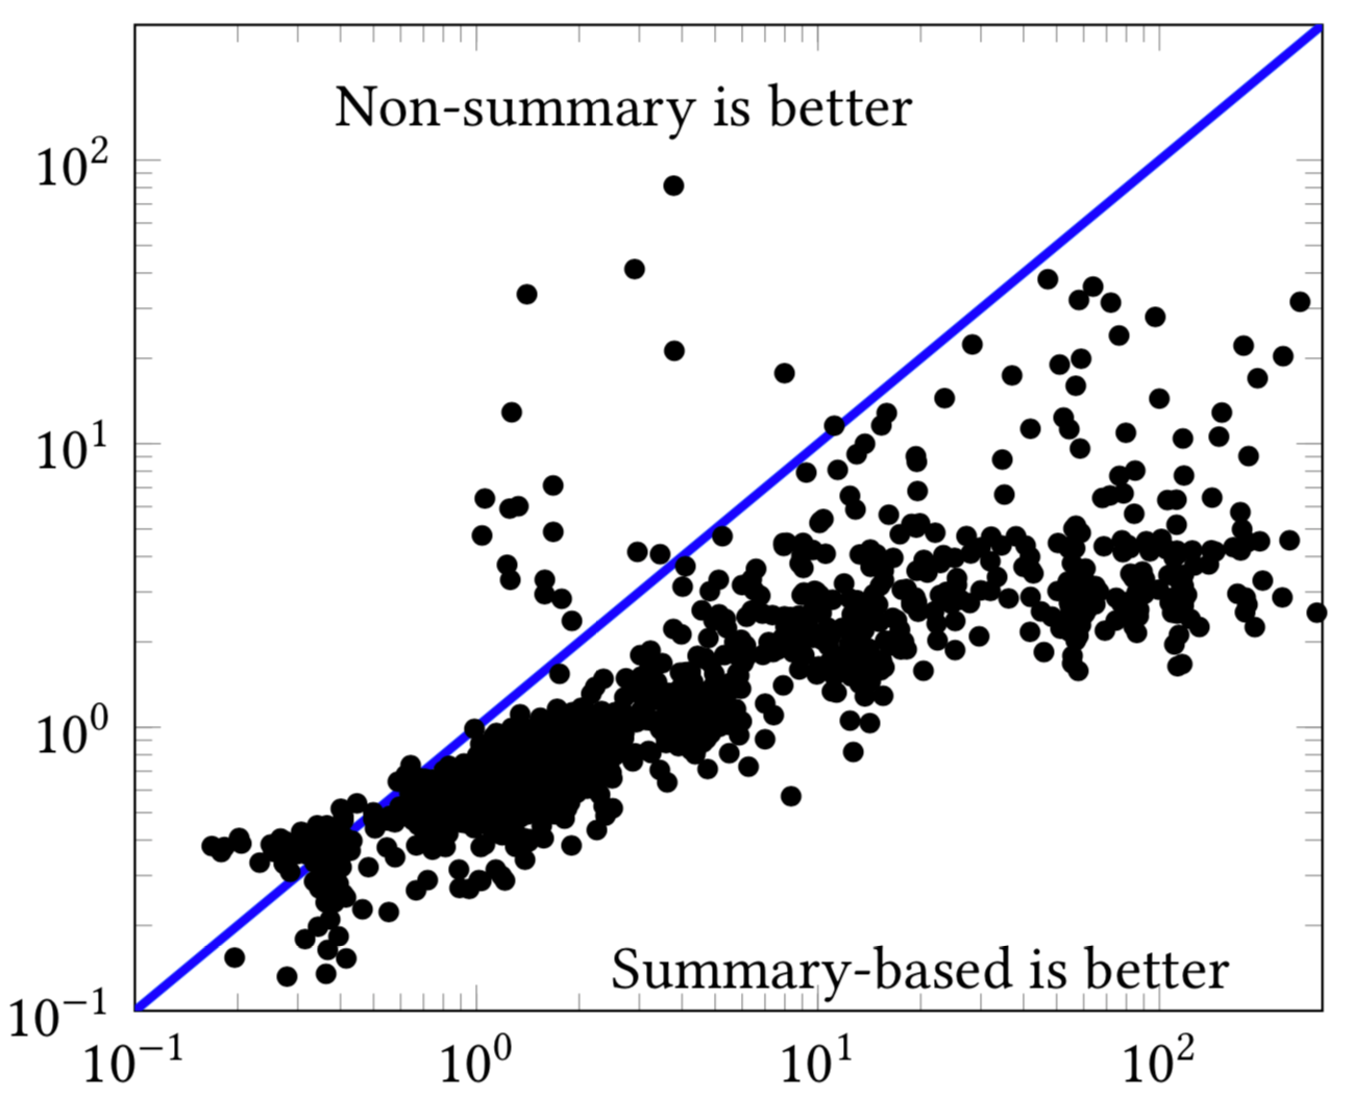
\includegraphics[scale=0.30]{sum-nosum.pdf}
% %   \vspace{-0.2in}
% \caption{Comparison of run times (in seconds) between non-summary (x-axis) and summary-based (y-axis) (log-scale).}
% % \vspace{-0.2in}
% \label{fig:plot-sum}
% \end{figure}

% \definecolor{bblue}{HTML}{0064FF}
\definecolor{rred}{HTML}{C0504D}
\definecolor{ggreen}{HTML}{9BBB59}
\definecolor{ppurple}{HTML}{9F4C7C}

\definecolor{b1}{HTML}{BEE9E8}
\definecolor{b2}{HTML}{188FA7}

\begin{figure}[!t]
\centering
\scalebox{0.85}{
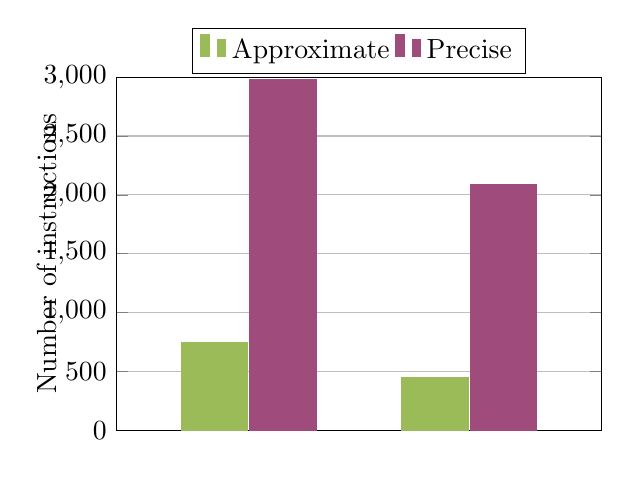
\begin{tikzpicture}
    \begin{axis}[
        width  = 8cm,
        height = 8cm,
        y=0.0015cm,
        x=2.8cm,
        major x tick style = transparent,
        ybar=2*\pgflinewidth,
        bar width=24pt,
        ymajorgrids = true,
        ylabel = {Number of instructions},
        ylabel style={yshift=-4mm},
        symbolic x coords={\batchoverflow,\reentrancy},
        ytick={0,500,1000,1500,2000,2500,3000},
        xtick = data,
        scaled y ticks = false,
        enlarge x limits=0.6,
        ymin=0,
        ymax=3000,
        legend cell align=left,
        legend entries={Approximate, Precise},
        legend style={
                at={(0.5,1.14)},
                legend columns=-1,
                anchor=north,
        %        column sep=1ex
        }
    ]
    %\hspace*{-2mm}
        \addplot[style={ggreen,fill=ggreen,mark=none}]
        coordinates{(\batchoverflow,743)(\reentrancy,451)};

        \addplot[style={ppurple,fill=ppurple,mark=none}]
        coordinates{(\batchoverflow,2976)(\reentrancy,2087)};
    \end{axis}
\end{tikzpicture}
}
% \vspace{-0.2in}
\caption{Average number of instructions evaluated under different settings}
\vspace{-0.2in}
\label{fig:eval-oyente}
\end{figure}

% \definecolor{bblue}{HTML}{0064FF}
\definecolor{rred}{HTML}{C0504D}
\definecolor{ggreen}{HTML}{9BBB59}
\definecolor{ppurple}{HTML}{9F4C7C}

\definecolor{b1}{HTML}{BEE9E8}
\definecolor{b2}{HTML}{188FA7}

\begin{figure}[!t]
\centering
\scalebox{0.85}{
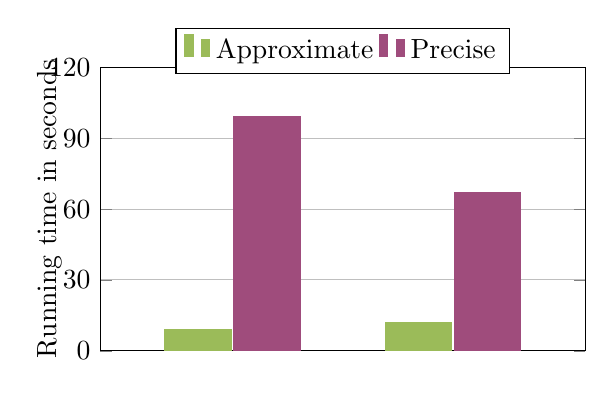
\begin{tikzpicture}
    \begin{axis}[
        width  = 8cm,
        height = 8cm,
        y=0.03cm,
        x=2.8cm,
        major x tick style = transparent,
        ybar=2*\pgflinewidth,
        bar width=24pt,
        ymajorgrids = true,
        ylabel = {Running time in seconds},
        ylabel style={yshift=-4mm},
        symbolic x coords={\batchoverflow,\reentrancy},
        ytick={0,30,60,90,120},
        xtick = data,
        scaled y ticks = false,
        enlarge x limits=0.6,
        ymin=0,
        ymax=120,
        legend cell align=left,
        legend entries={Approximate, Precise},
        legend style={
                at={(0.5,1.14)},
                legend columns=-1,
                anchor=north,
        %        column sep=1ex
        }
    ]
    %\hspace*{-2mm}
        \addplot[style={ggreen,fill=ggreen,mark=none}]
        coordinates{(\batchoverflow,9)(\reentrancy,12)};

        \addplot[style={ppurple,fill=ppurple,mark=none}]
        coordinates{(\batchoverflow,99)(\reentrancy,67)};
    \end{axis}
\end{tikzpicture}
}
% \vspace{-0.2in}
\caption{Average running time under different settings}
\vspace{-0.2in}
\label{fig:eval-oyente}
\end{figure}


\begin{table}[]
\begin{tabular}{|l|l|l|l|l|}
\hline
\multicolumn{1}{|c|}{\multirow{2}{*}{Statistics}} & \multicolumn{2}{l|}{\reentrancy} & \multicolumn{2}{l|}{\batchoverflow} \\ \cline{2-5} 
\multicolumn{1}{|c|}{}                         & $\vulnerability$             & $\vulnerability^{\diamond}$             & $\vulnerability$                & $\vulnerability^{\diamond}$               \\ \hline \hline  
Avg time (seconds)                                          &      9          &    52            &         12         &      67           \\ \hline
Avg \#instructions      &     451           &    1762            &         743         &      2087           \\ \hline
FPs                                             &           3\%     &       1\%         &    8\%              &         5\%        \\ \hline
FNs                                             &         7\%       &          23\%      &   5\%               &       32\%          \\ \hline
\end{tabular}
  \caption{Effectiveness of summary-based evaluation under queries of different granularity.}
%   \vspace{-0.3in}
  \label{tbl:summary}
\end{table}


Table~\ref{tbl:summary} shows the results of running \toolname with 
different settings and a time limit of 10 minutes. In particular, for the \reentrancy client, the approximate query $\vulnerability$ discussed in Section~\ref{sec:vul} has an average running time of 9 seconds while a precise query $\vulnerability^{\diamond}$ has to run for 52 seconds on average. Looking into the results closely, the approximate query $\vulnerability$ significantly reduces the size of the summaries. Specifically, $\vulnerability$ evaluates about 451 instructions on average while $\vulnerability^{\diamond}$ has to evaluate 1762 instructions on average. As a result, $\vulnerability^{\diamond}$ generates more false negatives (i.e., 23\% vs. 7\%) because it fails to explore enough search space within the time limit. On the other hand, although $\vulnerability$ is less precise, its false positive rate is very close to the one in $\vulnerability^{\diamond}$ (i.e., 3\% vs. 1\%). In the \batchoverflow client, we observe a similar trend.
\looseness=-1

% Each dot in the 
% figure represents the pairwise running time of a specific benchmark under different 
% settings; a dot near the diagonal indicates that the performance of 
% two settings is similar. Our summary-based symbolic
% evaluation significantly outperforms the baseline (i.e., non-summary) in the vast majority of benchmarks.
% As shown in Table~\ref{fig:summary},  if we exclude the benchmarks that timeout
% in 10 minutes, the mean time of our summary-based symbolic evaluation is only 8
% seconds, while it takes 35 seconds without computing the summary. Furthermore,
% 1846 benchmarks time out for both settings, and only 548 benchmarks time out on
% $S^{\dagger}$ but not on $S^{\diamond}$. However, without computing the summary,
% 17454 (i.e., 69.8\%) benchmarks time out. The result confirms that the
% summary-based technique is key to the efficiency of \toolname.\looseness=-1
% the running time of each benchmark under two different settings, and 
% the x-axis and y-axis represent the running time with and without computing 
% the summary, respectively. In particular, without computing the summary, on average
% it takes our tool \todo{XX} seconds to solve each benchmark and \todo{YY}
% benchmarks fail to terminate within a \todo{6} mins timeout. On the other hand, 
% the performance of our summary-based technique \emph{significantly} outperforms
% the baseline, and on average it takes only \todo{16} to solve each benchmark
% and timeouts on \todo{XXX} benchmarks.

\fbox{
\begin{minipage}{0.9\linewidth}
{\bf Result for RQ2:}
Summary-based technique is key to the efficiency of \toolname. In the meantime, the approximate queries enable \toolname to generate smaller summaries, which leads to much better scalability in exchange of a minor loss in precision.
\end{minipage}
} \\

% \subsection{A case study on the BatchOverflow vulnerability}\label{sec:case}

To evaluate whether \toolname can express and discover new vulnerabilities in real world
smart contracts, we conduct a case study on the recent \batchoverflow
vulnerability. Exploits
due to this vulnerability have resulted in the creation of trillions of invalid
Ethereum Tokens in 2018~\cite{batch-news}, causing major exchanges to temporary
halt until all tokens could be reassessed. Note that generating exploits for
this vulnerability is quite challenging as it requires the tool to reason about
the combination of arithmetic operations, interference, and the read-write
semantics of the storage system in Solidity. 
% For instance, existing tools such
% as \oyente and \madmax~\cite{madmax} will simply mark a large number of arithmetic
% operations as \emph{potentially vulnerable}, and it turns out that most of the
% alarms are not exploitable.

Similar to our previous experiment, we first encode the \batchoverflow vulnerability
(Section~\ref{sec:vul}) in our query language and then run our tool on the 
\etherscan data set. In total, \toolname flags 16 vulnerable
contracts. To verify that the exploits are effective, we setup a private
blockchain using the Geth~\cite{geth} framework where we can run exploits on the
vulnerable contracts. We confirmed that 9 exploits are valid. 
The infeasible attacks come from the incompleteness of the query 
as well as imprecise control flow graphs from the Vandal decompiler. 
Running \teether on these 9 vulnerable contracts, we find 
that it fails to generate their exploits.

% \todo{To evaluate the effectiveness of \toolname on vetting the \batchoverflow vulnerability, we compare \toolname against \teether~\cite{teether} tool, the most recent
% tool using dynamic symbolic execution for generating exploits that would enable
% the attacker to control the money transactions of a victim contract. In
% particular, the \teether tool looks for so-called \emph{critical instructions}
% (i.e., \texttt{call}, \texttt{selfdestruct}, etc.) that include recipients' addresses, 
% which can be manipulated by the attacker. In the end, \teether takes an average of 31 seconds to analyze the \etherscan data set but fails to generate exploits for those 9 vulnerable contracts. The false negative rate in \teether is caused by  
% attack programs that require more than three method calls, or victim programs with over 3000 lines of source code with complex control flow.
% As a result, the \teether tool fails to explore sufficiently many \emph{concrete traces} to 
% find the exploits.}  

